%Hier den Inhalt mit \input einfügen und die folgenden Zeilen entfernen

%\input{nomenclature.tex}

%\setcounter{section}{-1}% set to Kapitel 0 % Macht Probleme, wenn zuvor schon \section{...} aufgerufen wurde z.B. bei Zusammenfügen von mehreren Modulen

\section{Wiederholung}
%\begin{frame}\ftx{\secname}
% Kapitel 1
\s{% Skript-only
    Um das frequenz- und zeitabhängige Verhalten elektrischer Netzwerke zu beschreiben, 
    werden in diesem Kapitel kurz einige wichtige Grundlagen zusammengefasst. 

    Zur Bearbeitung vorrausgesetzt werden Kenntnisse über elektrische Grundgrößen, 
    lineare passive Bauteile $R$, $L$ und $C$, Netzwerkberechnungen, 
    sowie die komplexe Wechselstromrechnung.
}
%\end{frame}

%%%%%%%%%%%%%%%%%%%%%%%%%%%%%%%%%%%%%%%%%%%%%%%%%%%%%%%%%%%%%%%%%%%%%%%%%%%%%%%%%%%%%

\subsection{Frequenzabhängigkeit elektrischer Bauelemente}
\begin{frame}\ftx{\subsecname}
\s{% Skript-only
    Rein ohmsche Widerstände $R$ können elektrische keine Energie speichern. 
    Spannungen und Ströme sind proportional zueinander und zu jedem Zeitpunkt in Phase.
    Das Verhalten ist zeit- und frequenzunabhängig.

    Induktivitäten $L$ und Kapazitäten $C$ hingegen können Energie speichern und abgeben.
    Dieser Vorgang ist inert (träge), benötigt also eine gewisse Zeit. 
    Dadurch verhalten sie sich frequenzabhängig. 

    Ströme und Spannungen stehen bei Induktivitäten und Kapazititäten in (zeitlich) differentiellem 
    linearen Verhältnis zueinander. Dadurch entsteht bei beiden Bauteiltypen eine Phasenverschiebung 
    zwischen Spannung und Strom von betragsmäßig $90\ \degree$.

    Abbildung \ref{fig:bauteile:phasenverschiebung} zeigt die Spannungs- und Stromverläufe für $R$, $L$ und $C$
    bei Erregung mit einer Wechselspannung $u_q = U \cdot \sin(\omega t)$ zum Vergleich.

    \begin{figure}[H]\centering
        \begin{subfigure}{0.68\textwidth}\centering
            \includegraphics{Tikz/pdf/plot_bauteile_phasenverschiebung_r.pdf}
        \end{subfigure}%
        \begin{subfigure}{0.28\textwidth}\centering
            \begin{tikzpicture}[x=1mm,y=1mm]\draw[draw=none] (-14,-14) rectangle (+14,+14);  \draw (-10,0) to [R,name=R,l=$R$,v=$u_R$,i=$i_R$,!vi,o-o] (10,0); \varronly{R}; \iarronly{R}; \end{tikzpicture}% R
        \end{subfigure}\hfill% newline
        \begin{subfigure}{0.68\textwidth}\centering
            \includegraphics{Tikz/pdf/plot_bauteile_phasenverschiebung_l.pdf}
        \end{subfigure}%
        \begin{subfigure}{0.28\textwidth}\centering
            \begin{tikzpicture}[x=1mm,y=1mm]\draw[draw=none] (-14,-14) rectangle (+14,+14);  \draw (-10,0) to [L,name=L,l=$L$,v=$u_L$,i=$i_L$,!vi,o-o] (10,0); \varronly{L}; \iarronly{L}; \end{tikzpicture}% L
        \end{subfigure}\hfill% newline
        \begin{subfigure}{0.68\textwidth}\centering
            \includegraphics{Tikz/pdf/plot_bauteile_phasenverschiebung_c.pdf}
            \caption{Strom- und Spannungsverläufe}
        \end{subfigure}%
        \begin{subfigure}{0.28\textwidth}\centering
            \begin{tikzpicture}[x=1mm,y=1mm]\draw[draw=none] (-14,-14) rectangle (+14,+14);  \draw (-10,0) to [C,name=C,l=$C$,v=$u_C$,i=$i_C$,!vi,o-o] (10,0); \varronly{C}; \iarronly{C}; \end{tikzpicture}% C
            \caption{Schaltsymbole}
        \end{subfigure}
        \caption{Phasenverschiebung bei $R$, $L$ und $C$}\label{fig:bauteile:phasenverschiebung}
    \end{figure}

    Aufgrund der Phasenverschiebung bei $L$ und $C$ oszilliert deren Leistung 
    (Energieaufnahme und -abgabe), ist über eine Periode gemittelt jedoch immer null.
    Induktivitäten und Kapazitäten können daher keine Wirkleistung, sondern nur Blindleistung
    verrichten, weshalb sie auch Blindwiderstände genannt werden.
}
\b{% Folien-only
    %3 AC Plots: u(t), i(t) mit $\varphi$ eingezeichnet für $R$, $L$, $C$
    \begin{minipage}{\textwidth}\centering
        \onslide<1->{%
        \begin{minipage}{0.68\textwidth}\centering
            \resizebox{0.7\textwidth}{!}{\includegraphics{Tikz/pdf/plot_bauteile_phasenverschiebung_r.pdf}}   % plot \onslide<1->{...}        <-- OVERLAY
        \end{minipage}%
        }%
        \begin{minipage}{0.28\textwidth}\centering
            \begin{tikzpicture}[x=1mm,y=1mm]\draw[draw=none] (-14,-14) rectangle (+14,+14);  \draw (-10,0) to [R,name=R,l=$R$,v=$u_R$,i=$i_R$,!vi,o-o] (10,0); \varronly{R}; \iarronly{R}; \end{tikzpicture}% R
        \end{minipage}\hfill% newline
        \onslide<2->{%
        \begin{minipage}{0.68\textwidth}\centering
            \resizebox{0.7\textwidth}{!}{\includegraphics{Tikz/pdf/plot_bauteile_phasenverschiebung_l.pdf}}   % plot \onslide<2->{...}        <-- OVERLAY
        \end{minipage}%
        }%
        \begin{minipage}{0.28\textwidth}\centering
            \begin{tikzpicture}[x=1mm,y=1mm]\draw[draw=none] (-14,-14) rectangle (+14,+14);  \draw (-10,0) to [L,name=L,l=$L$,v=$u_L$,i=$i_L$,!vi,o-o] (10,0); \varronly{L}; \iarronly{L}; \end{tikzpicture}% L
        \end{minipage}\hfill% newline
        \onslide<3->{%
        \begin{minipage}{0.68\textwidth}\centering
            \resizebox{0.7\textwidth}{!}{\includegraphics{Tikz/pdf/plot_bauteile_phasenverschiebung_c.pdf}}   % plot \onslide<3->{...}        <-- OVERLAY
        \end{minipage}%
        }%
        \begin{minipage}{0.28\textwidth}\centering
            \begin{tikzpicture}[x=1mm,y=1mm]\draw[draw=none] (-14,-14) rectangle (+14,+14);  \draw (-10,0) to [C,name=C,l=$C$,v=$u_C$,i=$i_C$,!vi,o-o] (10,0); \varronly{C}; \iarronly{C}; \end{tikzpicture}% C
        \end{minipage}
    \end{minipage}
}% end Folien-only
\end{frame}

%%%%%%%%%%%%%%%%%%%%%%%%%%%%%%%%%%%%%%%%%%%%%%%%%%%%%%%%%%%%%%%%%%%%%%%%%%%%%%%%%%%%%

\subsubsection{Verhalten von Induktivitäten und Kapazitäten}
\begin{frame}\ftx{\subsubsecname}
\s{% Skript-only
    Induktivitäten als ideale Bauteile speichern durch den Effekt der (Selbst-)Induktion Energie im Magnetfeld.
    Kapazitäten als ideale Bauteile hingegen speichern Energie im elektrischen Feld. 
    Beschrieben werden beide Effekte durch das Induktion- beziehungsweise das Gaußsche Gesetz.

    Tabelle \ref{tab:vergleich:induktivitaetkapazitaet} listet die wichtigsten Unterschiede 
    im Verhalten von Induktivitäten und Kapazitäten qulitativ als Übersicht auf.

    \begin{table*}[h]\centering
    \caption{Vergleich von Induktivität und Kapazität im Verhalten}
    \label{tab:vergleich:induktivitaetkapazitaet}
    \begin{tabular}{ccc}
        \toprule&\textbf{Induktivität} &\textbf{Kapazität}\\
        \midrule
        \textbf{Gesetz}         &Induktionsgesetz       &Gaußsches Gesetz   \vphantom{$\Big|$}\\
        \textbf{Energiespeich.} &im Magnetfeld          &im Elektr. Feld    \vphantom{$\Big|$}\\
        \textbf{stetig}         &Strom                  &Spannung           \vphantom{$\Big|$}\\
        \textbf{bei Gleichspg.} &Kurzschluss            &offen              \vphantom{$\Big|$}\\
        \textbf{bei Hochfreq.}  &offen                  &Kurzschluss        \vphantom{$\Big|$}\\
        \bottomrule
    \end{tabular}
    \end{table*}

    Die (Selbst-)Induktivität $L$ als Eigenschaft kann vereinfacht als \glqq Trägheit \grqq des Stroms
    betrachtet werden. Ströme in Induktivitäten sind stetig und eilen der Spannung hinterher.
    Bei hohen Frequenzen sperrt die Induktivität, bei Gleichspannung verhält sie sich wie ein Kurzschluss.
    
    Die Kapazität $C$ kann dem gegenüber vereinfacht als \glqq Trägheit \grqq der Spannung betrachtet werden.
    Spannungen in Kapazitäten sind stetig und eilen dem Strom hinterher. 
    Bei Gleichstrom sperrt die Kapazität, bei hohen Frequenzen verhält sie sich wie ein Kurzschluss.

    \begin{figure}[H]\centering
        \begin{subfigure}{0.45\textwidth}\centering
            \includegraphics[width=0.75\textwidth]{./Bilder/Spule.png}
        \end{subfigure}%
        \begin{subfigure}{0.45\textwidth}\centering
            \includegraphics[width=0.75\textwidth]{./Bilder/Kondensator.png}
        \end{subfigure}
        \caption{Reale Induktivät (Spule, links) und Kapazitäten (Kondensator, rechts)}\label{fig:bauteile:realebauteile}
    \end{figure}
    Abbildung \ref{fig:bauteile:realebauteile} zeigt reale Bauteile, die Induktivitäten und Kapazitäten realisieren. 
    Gezeigt sind eine Spule (Induktivität) und ein Kondensator (Kapazität).
}
\b{% Folien-only
\begin{columns}
\column{0.5\textwidth}
    
    \textbf{Induktivität} \begin{tikzpicture}\draw (0,0) to [L,l=$L$] (2,0); \end{tikzpicture}
    \begin{itemize}
%           \item $L = \frac{\Phi}{i}$, mit $\Phi$ als magnetischer Fluss
        \item Impedanz: $\underline{Z}_{\mathrm L} = \mathrm{j}\omega L$
        \item DGL: $\ecv{u_{\mathrm L}} = L \cdot \frac{\d}{\d t}\, \eci{i_{\mathrm L}}$
        \item Energie im Magnetfeld
        \item Ströme stetig (keine Sprünge)
    \end{itemize}

    \textbf{Kapazität} \begin{tikzpicture}\draw (0,0) to [C,l=$C$] (2,0); \end{tikzpicture}
    \begin{itemize}
        \item Impedanz: $\underline{Z}_{\mathrm C} = -\mathrm{j}\frac{1}{\omega C}$
        \item DGL: $\eci{i_{\mathrm C}} = C \cdot \frac{\d}{\d t}\, \ecv{u_{\mathrm C}}$
        \item Energie im elektrischen Feld
        \item Spannungen stetig (keine Sprünge)
    \end{itemize}

% video: 
% nicht überall Sprünge vorgeben können

\column{0.5\textwidth}
    \begin{figure}[H]\centering
        \includegraphics[width=0.5\textwidth]{./Bilder/Spule.png}
        \par Spule
    \end{figure}
    \begin{figure}\centering
        \includegraphics[width=0.5\textwidth]{./Bilder/Kondensator.png}
        %\includegraphics[width=0.5\textwidth]{./Bilder/Kondensator_cut.png}
        \par Kondensator
    \end{figure}
\end{columns}
}% end Folien-only
\end{frame}

%%%%%%%%%%%%%%%%%%%%%%%%%%%%%%%%%%%%%%%%%%%%%%%%%%%%%%%%%%%%%%%%%%%%%%%%%%%%%%%%%%%%%

\subsubsection{Vergleich der linearen Zweipole $R$, $L$ und $C$}
\begin{frame}\ftx{\subsubsecname}

    \s{\ref{tab:vgl:bauteile:rlc} zeigt eine Gegenüberstellung der Größen $R$, $L$ und $C$ und fasst deren wichtigsten Eigenschaften zusammen. }

    % TODO: resizebox für beamer
    % TODO: "Symbol" vertical centering
    % ref: https://tex.stackexchange.com/questions/113022/vertical-alignment-in-tabular-cells-with-variable-height
    % TODO: try \usepackage{tabularx} % column width similar
    \begin{table}[h]\centering%
    \s{\caption{Vergleich lineare Bauteile $R$, $L$, $C$}\label{tab:vgl:bauteile:rlc}}%
    \resizebox{\textwidth}{!}{% for beamer page fit
    \begin{tabular}{ |c|c|c|c|c| }
        \hline &&&&\\[-6pt]
        \textbf{Größe}                          % Col 1
                & \textbf{Allgemein}            % Col 2
                & \textbf{El. Widerstand}       % Col 3
                & \textbf{Induktivität}         % Col 4
                & \textbf{Kapazität} \\[+4pt]   % Col 5
        \hline%
        %\textbf{Symbol}% outcommented, due to no vertical centering
        \begin{tikzpicture}[x=1mm,y=1mm]\draw[draw=none] (-14,-7) rectangle (+14,+7); \node[draw=none,align=center] {\textbf{Symbol}};\end{tikzpicture}
        %\begin{tikzpicture}[x=1mm,y=1mm]\draw[draw=black] (0,0) rectangle (5,5); \draw (2,2) node{S}; % DEBUG WIP 
                % tikzpicture           scaling   \draw     boundbox for same sized pictures    \draw   Bauteil
                & \begin{tikzpicture}[x=1mm,y=1mm]\draw[draw=none] (-14,-7) rectangle (+14,+7); \node[draw=none,align=center] {Zweipol\\Eintor};
                        \draw(0,0) node[dipchip, hide numbers, num pins=4, no topmark, external pins width=0](A){}; % Mittelpunkt des Zweipols
                        \draw(0,0) node[dipchip, hide numbers, num pins=2, no topmark, external pins width=0, opacity=0](B){}; % Ref. Pins mittig
                        \draw(B.bpin 1) to[short,-o] ++(-5,0);
                        \draw(B.bpin 2) to[short,-o] ++(5,0);
                  \end{tikzpicture}
                %& \begin{tikzpicture}[x=1mm,y=1mm]\draw[draw=none] (-4,-5) rectangle (+24,+7);  \draw (5,-5) rectangle (15,5); \draw (10,0) node{Bipol}; 
                %                                                                                \draw (0,0) to [short,o-] (5,0); 
                %                                                                                \draw (15,0) to [short,-o] (20,0); \end{tikzpicture}
                & \begin{tikzpicture}[x=1mm,y=1mm]\draw[draw=none] (-14,-7) rectangle (+14,+7);  \draw (-10,0) to [R,l=$R$,o-o] (10,0); \end{tikzpicture}
                & \begin{tikzpicture}[x=1mm,y=1mm]\draw[draw=none] (-14,-7) rectangle (+14,+7);  \draw (-10,0) to [L,l=$L$,o-o] (10,0); \end{tikzpicture}
                & \begin{tikzpicture}[x=1mm,y=1mm]\draw[draw=none] (-14,-7) rectangle (+14,+7);  \draw (-10,0) to [C,l=$ $,o-o] (10,0); 
                                                                                                \draw (5,3) node{$C$}; \end{tikzpicture} \\[+4pt]
        \hline &&&&\\[-6pt]
        %\textbf{Bauteil}
        %        & Dipol
        %        & Widerstand
        %        & Spule
        %        & Kondensator \\[+4pt]
        %\hline &&&&\\[-6pt]
        \textbf{Einheit}
                & $ \left[\textit{Form.z.}\right] = \mathrm{Einheit} $ 
                & $ \left[R\right] = \Omega\ \text{(Ohm)} $     
                & $ \left[L\right] = \mathrm{H}\ \text{(Henry)} $ 
                & $ \left[C\right] = \mathrm{F}\ \text{(Farad)} $ \\[+4pt]
        \hline &&&&\\[-6pt]
        \textbf{Zeitbereich}
                & $ \frac{\d}{\d t} $ bzw. $ \int \d t $ 
                & $ \ecv{u_{\mathrm{R}}} = R \cdot \eci{i_{\mathrm R}} $     
                & $ \ecv{u_{\mathrm{L}}} = L \cdot \frac{\d}{\d t}\, \eci{i_{\mathrm{L}}} $ 
                & $ \eci{i_{\mathrm{C}}} = C \cdot \frac{\d}{\d t}\, \ecv{u_{\mathrm{C}}} $ \\[+4pt]
        \hline &&&&\\[-6pt]
        \textbf{Frequenzb.}
                & $ \mathrm{j}\omega $ bzw. $ \frac{1}{\mathrm{j}\omega} $
                & $ \ecv{\underline{U}_{\mathrm R}} = R                   \cdot \eci{\underline{I}_{\mathrm R}} $ 
                & $ \ecv{\underline{U}_{\mathrm L}} = \mathrm{j}\omega L  \cdot \eci{\underline{I}_{\mathrm L}} $
                & $ \eci{\underline{I}_{\mathrm C}} = \mathrm{j}\omega C  \cdot \ecv{\underline{U}_{\mathrm C}} $ \\[+4pt]
        \hline &&&&\\[-6pt]
        \textbf{Impedanz}
                & $ \underline{Z} = \frac{\ecv{\underline{U}}}{\eci{\underline{I}}} $
                & $ \underline{Z}_{\mathrm R} = R $ 
                & $ \underline{Z}_{\mathrm L} = \mathrm{j}\omega L $
                & $ \underline{Z}_{\mathrm C} = -\mathrm{j}\frac{1}{\omega C} $ \\[+4pt]
        \hline &&&&\\[-6pt]
        \textbf{Wirkanteil}
                & $ R = \Re\{\underline{Z}\} $
                & $ R = \frac{U}{I} $
                & $ 0 $
                & $ 0 $ \\[+4pt]
                \hline &&&&\\[-6pt]
        \textbf{Blindanteil}
                & $ X = \Im\{\underline{Z}\} $
                & $ 0 $
                & $ X_{\mathrm L} = \omega L $
                & $ X_{\mathrm C} = -\frac{1}{\omega C}$ \\[+4pt]
        \hline
    \end{tabular}
    } % end resizebox
    \end{table}
    
% Für Schaltungen variabler Frequenz: Frequenzvariablen Eigenschaften von Bauteilen, dafür zeitvariante 
\end{frame}

%%%%%%%%%%%%%%%%%%%%%%%%%%%%%%%%%%%%%%%%%%%%%%%%%%%%%%%%%%%%%%%%%%%%%%%%%%%%%%%%%%%

% Beschreibe in Textform wie das Verhalten von Eingangs- zu Ausgangssignalen eines Vierpols 
% mithilfe des Frequenzgangs (bzw. des Amplituden- und Phasengangs) beschrieben werden kann
\s{
\subsection{Zweitore (Vierpole)}
\begin{frame}\ftx{\subsecname}


    % Wiederholung Eintor
    Die Frequenzabhängigkeit von Eintoren (Zweipole) haben wir in Modul 3 bereits untersucht.  
    Mithilfe der komplexen Wechselstromrechnung konnten wir den frequenzabhängigen Wechselstromwiderstand 
    (Impedanz) $\underline{Z}$ einzelner Eintore bestimmen. Durch Anwendung der komplexen Strom- 
    und Spannungsteilerregel konnten wir auch die Gesamt-Impedanz linearer zweipoliger Netzwerke bestimmen. 
    Das heißt für solche, welche nur aus linearen Bauteilen wie $R$, $L$ und $C$ bestehen. 

    % Tikzpicture: Vergleich Vierpol und Zweipol
    %
    % Zeichne links einen senkrechten Zweipol mit Spannungs- (U) und Strompfeil (I) jeweils von oben nach unten
    % Zeichne rechts einen Vierpol (Eingangspole links, Ausgangspole rechts) (U1 links oben nach unten, U2 rechts oben nach unten)
    \begin{figure}[h]
        \begin{subfigure}{0.48\textwidth}\centering
            \includegraphics{Tikz/pdf/circ_eintor.pdf}
        \end{subfigure}\hfill
        \begin{subfigure}{0.48\textwidth}\centering
            \includegraphics{Tikz/pdf/circ_zweitor.pdf}
        \end{subfigure}
        \caption{Vergleich: Schaltzeichen eines allgemeinen Zwei- und Vierpols}
        \label{fig:vgl:zweipolvierpol}
    \end{figure}

    % Einführung Zweitor, wozu
    Zweitore (Vierpole) sind eine Erweiterung von Eintoren (Zweipolen).
    Sie verfügen über eine Eingangs- und eine Ausgangsseite mit jeweiligen Eingangs- und Ausgangsgrößen.  
    Das Zweitormodell eignet sich gut zur Beschreibung von (frequenzabhängigen) Übertragungseigenschaften 
    von elektrischen Netzwerken. 

    \fu{\includegraphics{Tikz/pdf/circ_zweitor_quelle_last.pdf}
    }{Verbindung einer Last über ein Zweitor mit der Quelle.\label{circ:quellezweitorlast}}% im Foliensatz im nächsten Kapitel (Freuqenzgang, Amplitudengang, Phasengang)
    
    Im einfachsten Fall wird wie in \ref{circ:quellezweitorlast} gezeigt, eine Quelle (Eintor) über ein Zweitor 
    mit einer Last (Eintor) verbunden. 
    Typische Zweitore sind beispielsweise Verstärker, Filter oder auch Transformatoren. 
\end{frame}
}% end skript only


    % Wiederholung
\newpage

%%%%%%%%%%%%%%%%%%%%%%%%%%%%%%%%%%%%%%%%%%%%%%%%%%%%%%%%%%%%%%%%%%%%%%%%%%%%%%%%%%%
%%%%%%%%%%%%%%%%%%%%%%%%%%%%%%%%%%%%%%%%%%%%%%%%%%%%%%%%%%%%%%%%%%%%%%%%%%%%%%%%%%%
%                               START KAPITEL 1 
%%%%%%%%%%%%%%%%%%%%%%%%%%%%%%%%%%%%%%%%%%%%%%%%%%%%%%%%%%%%%%%%%%%%%%%%%%%%%%%%%%%
%%%%%%%%%%%%%%%%%%%%%%%%%%%%%%%%%%%%%%%%%%%%%%%%%%%%%%%%%%%%%%%%%%%%%%%%%%%%%%%%%%%

\section[Einführung]{Einführung in Schaltvorgänge}
\label{sec:einfuehrung}
\begin{frame}\ftx{\secname}
\s{%
	% Einführung 
	Schaltvorgänge sind Ausgleichsvorgänge, welche unmittelbar nach dem Schalten in elektrischen Netzwerken auftreten.
	Wie der Begriff \glqq elektrische Schaltung\grqq\ im Deutschen vermuten lässt, spielt das Schalten eine große Rolle in der Elektrotechnik. 
	Selbst elektrische Netzwerke, in denen nicht geschalten wird, werden gemeinhin als Schaltungen bezeichnet.

	% Beispiele
	Schalter finden vielfältig Anwendung unter anderem in der Leistungselektronik, der Informations-, der Kommunikations- 
	und der Regelungstechnik. Dabei kommt es nach jedem effektiven Schalten zu Ausgleichsvorgängen, 
	die mitunter erwünschte oder unerwünschte Effekte hervorrufen können.

	% Themen Eingrenzung
	In diesem Modul liegt der Fokus auf der Untersuchung dieser Ausgleichsvorgänge.
}
\begin{Lernziele}{Einführung}
	Studierende lernen: 
	\begin{itemize}
		\item Schaltvorgänge als nicht-stationäre Zustände nach Schaltaktionen kennen % Wissen
		\item Schaltvorgänge im Kontext anderer Ausgleichsvorgänge zu verstehen % Verstehen
		\item Herausforderungen und Möglichkeiten bei Schaltvorgängen kennen % Wissen, Anwenden (Beispiele Praxis, LE, Filter, Verzögerungen, ...)
		\item das Schaltverhalten von idealen und realen Schaltern zu unterscheiden % Verstehen
	\end{itemize}
\end{Lernziele}
\end{frame}



%%%%%%%%%%%%%%%%%%%%%%%%%%%%%%%%%%%%%%%%%%%%%%%%%%%%%%%%%%%%%%%%%%%%%%%%%%%%%%%%%%%%%%%%%%%%%%%%%%

\subsection{Ausgleichsvorgänge}
\label{sec:einfuehrung:ausgleichsvorgaenge}
\begin{frame}\ftx{\subsecname}
\s{%
	% Vorstellung: Ausgleichsvorgänge
	Ausgleichsvorgänge sind allgemein Vorgänge, in denen ein System nach einer Störung einem Gleichgewichtszustand zustrebt.
	
	% Analogien
	Ein Blick in die Physik zeigt, dass Ausgleichsvorgänge auf mannigfaltige Art und Weise in vielen Bereichen vorkommen. 
	Nach dem zweiten Hauptsatz der Thermodynamik strebt ein System stets einem Gleichgewichtszustand zu.
	Demnach kann jeder Vorgang bei entsprechenden Systemgrenzen als Ausgleichsvorgang betrachtet werden.
	Ein Stückweit lassen sich Schaltvorgänge mittels Analogien zu anderen Ausgleichsvorgängen beschreiben.  
	% Alle Vorgänge? 2. Satz Thermodynamik -> Makroskopisch? ... Mh...
	
	% Beispiele
	Beispiele für Ausgleichsvorgänge sind das Erhitzen einer Flüssigkeit, das Ausschwingen eines Pendels oder der Regelvorgang eines Regelkreises.

	\begin{figure}[H]\centering
		% Bild: Bartolomeo Pinelli, Ausschnitt aus \textit{A Peasant Family Cooking over a Campfire}, CC0 1.0. \url{https://commons.wikimedia.org/w/index.php?curid=81414513}
		\includegraphics[width=0.3\textwidth]{Bilder/Ausschnitt_A_Peasant_Family_Cooking_over_a_Campfire_by_Bartolomeo_Pinelli_CC0_1.0.png} % 320x319px
		\caption{Erhitzen einer Flüssigkeit\protect\footnotemark}\label{fig:einfuehrung:ausgleichsvorgang:temperaturausgleich}
	\end{figure}
	\footnotetext{Bartolomeo Pinelli, Ausschnitt aus \textit{A Peasant Family Cooking over a Campfire}, Lizenz CC0 1.0\newline\qquad\url{https://commons.wikimedia.org/w/index.php?curid=81414513}}
		
	%Beispiel aperiodisch (DGL 1. Ordnung):\\
	%	Temperaturausgleich. Warum? Energieniveaus anschaulich und Irreversibilität (Entropiesteigerung) (klassisch)

	%Beispiel periodisch (DGL 2. Ordnung):\\
	%	Federpendel. Passt zu \glqq Einschwingvorgängen\grqq. (klassisch)

	%Beispiel periodisch (DGL 2. Ordnung):\\ 
	%	Vergleich Regelung (Motorik). Passt, weil rechnerisch gleich und abgedeckt in Definition ($\rightarrow$ stationärer Zustand)
	%	(Praktisch wegen Überschwingen)
}%
\b{%
	\begin{minipage}{\textwidth}% Obere Hälfte
		\begin{minipage}{0.48\textwidth}\centering
			\resizebox{0.9\textwidth}{!}{\includegraphics{Tikz/pdf/circ_switchable_rc_charge_dc.pdf}}
		\end{minipage}%
		\begin{minipage}{0.48\textwidth}\centering
			\includegraphics{Tikz/pdf/plot_rc_charge_uc_transition.pdf}
		\end{minipage}
	\end{minipage}
	\vspace{0.5cm}
	\pause

	\begin{minipage}{\textwidth}% Untere Hälfte
		\begin{minipage}[t]{0.48\textwidth}\centering
			\underline{Analogie: Wasser erhitzen}\footnotemark
			\vspace{2mm}

			\includegraphics[width=0.4\textwidth]{Bilder/Ausschnitt_A_Peasant_Family_Cooking_over_a_Campfire_by_Bartolomeo_Pinelli_CC0_1.0.png}%
			\pause
		\end{minipage}%
		\begin{minipage}[t]{0.48\textwidth}%\centering
			\underline{Ursachen für Ausgleichsvorgänge:}
			\vspace{2mm}
			\begin{itemize}
				\item Schalthandlungen
				\item DC: Änderung d. Spannung/Strom
				\item AC: Änderung d. Frequenz/Amplitude/Phase
			\end{itemize}
		\end{minipage}
	\end{minipage}
	\footnotetext{Bild: Bartolomeo Pinelli, Ausschnitt aus \textit{A Peasant Family Cooking over a Campfire}, Lizenz CC0 1.0\newline\qquad\url{https://commons.wikimedia.org/w/index.php?curid=81414513}}
}
\end{frame}

\b{% Beamer only, extra frame
\begin{frame}\ftx{\subsecname\,- Beispiele}
	\includegraphics[width=\textwidth]{Bilder/Ausgleichsvorgaenge_Beispiele_ET3_S_Exknowski_FH_SWF.png}% Provisorisch mit Genehmigung von Prof. Exknowski
\end{frame}
}
%%%%%%%%%%%%%%%%%%%%%%%%%%%%%%%%%%%%%%%%%%%%%%%%%%%%%%%%%%%%%%%%%%%%%%%%%%%%%%%%%%%%%%%%%%%%%%%%%%

\subsection{Schaltvorgänge}
\label{sec:einfuehrung:schaltvorgaenge}
\begin{frame}\ftx{\subsecname}
\s{
	% Def: Schaltvorgang, Prämisse (idealer Schalter)
	Als Schaltvorgänge werden Ausgleichsvorgänge unmittelbar \underline{nach} dem Schalten bezeichnet.
	Diese sind Hauptgegenstand des Moduls, wobei hierfür stehts von idealen Schaltern ausgegangen wird.

	% Bild: Schaltvorgang DC, AC
	Abbildung \ref{fig:plot:transient_persistent} zeigt exemplarisch den Zeitverlauf einer 
	Systemgröße $s(t)$ (z.B. Strom oder Spannung) während eines Schaltvorgangs. 
	Zum Vergleich sind für das Zuschalten einer Anregung zwei Fälle dargestellt:
	einmal für eine Gleichgröße (DC) und einmal für eine Wechselgröße (AC).
}
% Bsp. Einschwingvorgang nach Schalten als Schaltvorgang. Vgl. DC und AC 
\b{\centering Beispiel Schaltvorgang bei Gleich- und Wechselspannung.
}%
\fu{\includegraphics{Tikz/pdf/plot_transient_persistent.pdf}}%
	{Vergleich: Ausgleichsvorgang AC, DC\label{fig:plot:transient_persistent}}
\s{
	% Bild-Erklärung: Vorgänge, Zustände
	% stationär -> Schalten (instantan) -> Schaltvorgang (transient) -> stationärer Zustand (persistent)
	Der dargestellte Schaltvorgang beginnt mit dem Schalten bei $t=0$ (gestrichelte Grenze, links) 
	und endet mit Erreichen eines stationären Zustands (persistent) (gestrichelte Grenze, mittig).
	Der stationäre Zustand von $s(t)$ entspricht
	bei Anregung mit Gleichgröße (DC) ebenfalls einer Gleichgröße (konstant) und
	bei Anregung mit Wechselgröße (AC) ebenfalls einer Wechselgröße (periodisch). 

	Der in Abb. \ref{fig:plot:transient_persistent} dargestellte Vorgang beim Übergang (transient) 
	von Schalten bis Erreichen eines stationären Zustands kann hier auch als 
	Ausgleichsvorgang (allgemein), Schaltvorgang (speziell) oder Einschwingvorgang (speziell) bezeichnet werden. 

	% Abgrenzung: Vorgänge beim Schalten (realer Schalter)
	Ausgleichsvorgänge \underline{während} dem Schalten, wie sie bei realen Schaltern auftreten,
	werden nicht als Schaltvorgänge bezeichnet und in diesem Modul nicht näher untersucht. 
	Eine kurze Erläuterung findet sich jedoch vollständigkeitshalber in Abschnitt \ref{sec:einfuehrung:schalteridealvsreal} 
	beim Vergleich idealer und realer Schalter.
}
\end{frame}

%%%%%%%%%%%%%%%%%%%%%%%%%%%%%%%%%%%%%%%%%%%%%%%%%%%%%%%%%%%%%%%%%%%%%%%%%%%%%%%%%%%%%%%%%%%%%%%%%%

\subsection{Beispiele für Schaltvorgänge}
\label{sec:einfuehrung:beispieleschaltvorgaenge}
\begin{frame}\ftx{\subsecname}
% Anwendungsbereiche von Schaltungstechnik: Leistungselektronik, Kommunikationstechnik(?), ...
\b{% Beamer only
\textbf{Beispiel aus der Leistungselektronik:} 

\begin{minipage}{0.38\textwidth}\centering
	\includegraphics[width=\textwidth]{Bilder/Tiefsetzsteller_Schaltung_GET2_J_Böcker_Uni_Paderborn_cut.png}
	Tiefsetzsteller mit Glättungskondensator\footnotemark
\end{minipage}%
\begin{minipage}{0.58\textwidth}\centering
	\includegraphics[width=0.9\textwidth]{Bilder/Tiefsetzsteller_Zeitverläufe_GET2_J_Böcker_Uni_Paderborn_cut_edit.png}
\end{minipage}
\footnotetext{Schaltbild und Zeitverlauf: Joachim Böcker, GET2, Universität Paderborn, modifiziert (gekürzt)}

Stromrichter (engl. \textit{power converter}) wandeln elektrische in elektrische Energie um 
Die Wandlung (z.B. Spannung, Strom, Frequenz) erfolgt durch getaktetes Schalten.\vspace{5pt}

\textbf{Andere Beispiele:}\\
Ein-/Ausschalten, AD-/DA-Converter, Fahrradlicht mit Kondensator, ...
}% end Beamer only
\s{% Skript only
	Prinzipiell kommt es bei jedem Schalten in elektrischen Netzwerken zu Schaltvorgängen. 
	
	Typische Beispiele sind Umrichter (engl. \textit{power converter}) in der Leistungselektronik,
	welche elektrische Energie in eine andere Form elektrischer Energie umwandeln. 
	Durch gezieltes Schalten von Halbleiterbauelementen (z.B. Transistoren, Thyristoren) 
	kann die Spannung, der Strom oder die Frequenz verändert werden. 
	In jedem Taktzyklus werden Kapazitäten und Indukivitäten abwechselnd geladen und entladen. 
	
	Abbildung \ref{fig:circ:pulldown} zeigt beispielhaft eine Tiefsetzsteller (Buck-Converter) mit Glättungskondensator.
	Dieser wandelt eine Gleichspannung $U_1$ in eine niedrigere Gleichspannung $U_2$ um. 
	Daneben sind in Abbildung \ref{fig:plot:pulldown} die zeitlichen Verläufe von Spannungen und Strömen
	jeweils am Eingang und am Ausgang des Tiefsetzstellers dargestellt.

	\begin{figure}[H]\centering
		\begin{subfigure}{0.5\textwidth}\centering
			\includegraphics[width=\textwidth]{Bilder/Tiefsetzsteller_Schaltung_GET2_J_Böcker_Uni_Paderborn_cut.png}
			\caption{Schaltbild eines Tiefsetzstellers (Buck-Converter)}
			\label{fig:circ:pulldown}
		\end{subfigure}%
		\begin{subfigure}{0.5\textwidth}\centering
			\includegraphics[width=0.9\textwidth]{Bilder/Tiefsetzsteller_Zeitverläufe_GET2_J_Böcker_Uni_Paderborn_cut_edit.png}
			\caption{Zeitverlauf von $u(t)$ und $i(t)$ am Tiefsetzsteller}
			\label{fig:plot:pulldown}
		\end{subfigure}
		\caption{Beispiel: Schaltvorgänge am Tiefsetzsteller\protect\footnotemark}
	\end{figure}
	\footnotetext{Quelle: Schaltbild und Zeitverlauf (modifiziert, gekürzt): Joachim Böcker, GET2, Universität Paderborn}

	Ohne nähere Rechnung ist erkennbar, dass die Ausgangsspannung auch im stationären Betrieb nicht konstant ist.
	Die Ausgangsspannung über dem Glättungskondensator schwankt, da sich die Kapazität in jeder Schaltperiode 
	etwas entlädt und wieder auflädt. 
	
	Mithilfe der Methoden aus diesem Modul lassen sich solche Schaltvorgänge berechnen und analysieren. 
	Zum besseren Verständnis werden in Kapitel \ref{sec:schaltvorgaengezeitbereich} jedoch einfachere Beispiele von
	Schaltvorgänge ohne periodisches Schalten betrachtet.

	Andere Beispiele für Schaltvorgänge sind das Ein- und Ausschalten von Geräten,
	Analog-Digital- und Digital-Analog-Wandlung, das Aufladen eines Kondensators durch ein Fahrradlicht.
}

	%Bei elektrischen Schaltvorgängen: Schalter (Ein/Aus), Relais, Transistoren, ...
%
	%Leistungselektronik überwiegend Schaltungselektronik im wortwörtlichen Sinne. 
	%%( DC <---DC/AC ---> AC)
	%%( î  .           .  î )
	%%( |    .       .    | )
	%%( |      .   .      | )
	%%(DC/DC     X     AC/AC)
	%%( |    .       .    | )
	%%( v  .           .  v )
	%%( DC <---DC/AC ---> AC)
%
	%DC/AC: Wechselrichter (U,f,phi)\\
	%AC/AC: Frequenzumrichter (f) / Phasenregler (phi) / AC-Spannungsregler (U,(f),(phi))\\
	%DC/DC: Hochsetz-/Tiefsetz-/Hochtiefsetz-steller / DC-Spannungsregler (U)\\
	%AC/DC: Gleichrichter (U)\\

\end{frame}

%%%%%%%%%%%%%%%%%%%%%%%%%%%%%%%%%%%%%%%%%%%%%%%%%%%%%%%%%%%%%%%%%%%%%%%%%%%%%%%%%%%%%%%%%%%%%%%%%%

\subsection{Idealer Schalter vs. Realer Schalter}
\label{sec:einfuehrung:schalteridealvsreal}
\begin{frame}\ftx{\subsecname}
\s{
	% Intro: Reales Schalten
	Das Öffnen oder Schließen (Schalten) eines Schalter selbst ist ein Vorgang, 
	welcher real betrachtet stets mit Latenzen und Verlusten einhergeht.
}
\begin{figure}[H]\centering
	\includegraphics{Tikz/pdf/circ_switch_ideal.pdf}
	\s{\caption{Schaltbild, Schalterspannung}}\b{\par Schalterspannung $\ecv{u(t)}$}
	\label{fig:circ:switch}
\end{figure}
\s{
	% Abbildung: Ideal vs. Real
	Abbildung \ref{fig:plot:schalter} zeigt zum Vergleich das Zeitverhalten 
	eines idealen und eines realen Schalter während dem Ein- und Ausschalten (Schließen und Öffnen).
	Dargestellt sind die Zeitverläufe der Spannung $u(t)$ über einen Schalter.
	Dabei sei eine Gleichspannung $U_q$ über dem Schalter angelegt.
}
\begin{figure}[H]\centering
	\begin{subfigure}{0.48\textwidth}\centering
		\includegraphics{Tikz/pdf/plot_switch_ideal.pdf}
		\s{\caption{Spannung bei idealem Schalter}}\b{\par Ideal: verlustlos, instantan}
		\label{fig:plot:schalter:ideal}
	\end{subfigure}\pause
	\begin{subfigure}{0.48\textwidth}\centering
		\includegraphics{Tikz/pdf/plot_switch_real.pdf}
		\s{\caption{Spannung bei realem Schalter}}\b{\par Real: Verluste, Latenzen}
		\label{fig:plot:schalter:real}
	\end{subfigure}
	\s{\caption{Vergleich: Schaltverläufe bei idealem und realem Schalter}}
	\label{fig:plot:schalter}
\end{figure}
%i(t),u(t)			ideal
%		î
%	U2_	|    ________         ______
%		|   |        |       |
%	U1_	|___|        |_______|
%		|___________________________> t
%
%i(t),u(t)			real
%		î
%	U2_	|..  _______   ....   ______    ___ = Spannung
%		|  ./       \.      ./
%	U1_	|__/ ....... \______/.......    ... = Strom
%		|___________________________> t
\end{frame}
\begin{frame}\ftx{\subsecname}
\s{
	% Beschreibung: Ideal vs. Real
	Ein idealer Schalter wechselt beim Schalten instantan und verlustlos 
	von einem leitenden Zustand ($R=0$) zu einem sperrenden Zustand ($G=0$) oder umgekehrt
	wie in Abbildung \ref{fig:plot:schalter:ideal} dargestellt ist.
	Ein realer Schalter hingegen leitet oder sperrt nicht instantan
	wie in Abb. \ref{fig:plot:schalter:real} vereinfacht dargestellt ist. 
	Das heißt, dass während des Schaltens bereits (oder noch) 
	eine Spannung anliegen kann, wodurch es zu Schaltverlusten kommen kann.
	
	% Erklärung
	Die Latenzen und Verluste realer Schalter resultieren aus deren resistiven, induktiven und kapazitiven Eigenschaften.
	Aufgrund dieser Eigenschaften ist Schalten real betrachtet - schalterintern - immer mit Ausgleichsvorgängen verbunden.
	In der Praxis werden solche Effekte, wenn unerwünscht, als parasitär bezeichnet.
	
	% Beispiel: MOSFET
	Abbildung \ref{fig:circ:mosfet} zeigt exemplarisch einen MOSFET als Schalter zur Veranschaulichung. 
	Zum Vergleich ist der MOSFET einmal ideale (ohne) und einmal real (mit kapazitiven Effekten) dargestellt.
}
% Ref: http://fmh-studios.de/theorie/mosfet/schaltverhalten/
\begin{figure}[H]\centering
	\begin{subfigure}{0.48\textwidth}\centering
		\includegraphics{Tikz/pdf/circ_mosfet_ideal.pdf}
		\s{\caption{MOSFET, ohne Kapazitäten (ideal)}}\b{Ideal: keine parasitären Effekte}
		\label{fig:circ:mosfet:ideal}
	\end{subfigure}%
	\onslide<2->{%
	\begin{subfigure}{0.48\textwidth}\centering
		\includegraphics{Tikz/pdf/circ_mosfet_capacitive_effects.pdf}
		\s{\caption{MOSFET, inkl. Kapazitäten (real)}}\b{Real: mit parasitären Kapazitäten}
		\label{fig:circ:mosfet:kapazitiv}
	\end{subfigure}
	}% end onslide
	\s{\caption{Vergleich: Schaltung mit MOSFET, ohne (ideal) und mit kapazitiver Effekte (real)}}
	\label{fig:circ:mosfet}
\end{figure}
\s{
	%Der MOSFET wird am Drain-Anschluss über einen Widerstand $R$ mit einer konstanten Gleichspannung ($5\ \mathrm{V}$ Potential) versorgt.
	%Das Potential am Source-Anschluss ist auf konstant $0\ \mathrm{V}$ gelegt. 
	%Die Eingangsspannung $\underline{U}_1$ liegt zwischen Gate und Source an,
	%die Ausgangsspannung $\underline{U}_2$ zwischen Drain und Source.

	% Erklärung Latenzen
	Die kapazitiven Effekte zwischen den Anschlüssen des MOSFETs führen zu einer Verzögerung beim Schalten,
	da die jeweiligen Kapazitäten während des Schaltens erst geladen beziehungsweise entladen werden müssen.
	
	% Abgrenzung
	Für die Berechnung von Schaltvorgängen wird in diesem Modul stets von idealen Schaltern ausgegangen.
	Das MOSFET-Beispiel dient lediglich zur Veranschaulichung der Unterschiede zwischen idealen und realen Schaltern.
	Ausgleichsvorgänge während des Schaltens werden in diesem Modul nicht weiter betrachtet. 
	Die vorgestellten Berechnungsmethoden für Schaltvorgänge lassen sich jedoch prinzipiell 
	auch auf diese anwenden.
}%
\b{%
	\makebox[2cm][l]{\textbf{Hier:}} Ausgleichsvorgänge \makebox[1.5cm][c]{\underline{nach}} Schalten (Schaltvorgänge) im Fokus
	%\\\qquad$\rightarrow$ Annahme idealer Schalter %(verlustlos, instantan)
	\\[+4pt]%
	\makebox[2cm][l]{\textbf{Real:}} Ausgleichsvorgänge \makebox[1.5cm][c]{\underline{während}} Schalten
	%\\\qquad$\rightarrow$ Schaltverluste und Latenzen
	\\[+4pt]%
	\makebox[2cm][l]{\textbf{Eingrenz.:}} Annahme idealer Schalter 
}
\end{frame}

%%%%%%%%%%%%%%%%%%%%%%%%%%%%%%%%%%%%%%%%%%%%%%%%%%%%%%%%%%%%%%%%%%%%%%%%%%%%%%%%%%%%%%%%%%%%%%%%%%

%\subsection{...}
%\label{sec:...}
%\begin{frame}\ftx{\subsecname}
%\end{frame}

%-------------------------------------------------------------------------------------------------%
    % Frequenzgang, Amplitudengang, Phasengang
\newpage

%%%%%%%%%%%%%%%%%%%%%%%%%%%%%%%%%%%%%%%%%%%%%%%%%%%%%%%%%%%%%%%%%%%%%%%%%%%%%%%%%%%
\section{Logarithmische Darstellung, Frequenzgang, Grenzfrequenz}
\label{sec:frequenzganglog}%
\begin{frame}\ftx{\secname}%
\s{\index{logarithmische Darstellung}%
    % Einleitung
    In der Elektrotechnik und Nachrichtentechnik werden häufig logarithmische Skalen verwendet,
    um den Frequenzgang von Filtern und Verstärkern darzustellen. Die logarithmische Darstellung
    ermöglicht eine bessere Übersicht über das Verhalten des Systems im gesamten Frequenzbereich.

    Abbildung \ref{fig:xkcd_logscale} zeigt zwei Comic-Strips von XKCD, die die Vorteile der logarithmischen
    Darstellung humorvoll darstellen.

    In diesem Kapitel werden wir uns mit der logarithmischen Darstellung von Frequenzgängen in Form sogenannter
    Bode-Diagramme beschäftigen. Zur Beschreibung des Frequenzganges einfacher Filterschaltungen werden
    die Einheit Dezibel, sowie die Grenzfrequenz und die Ordnung von Filtern definiert.
    Darüber hinaus werden Bandpass- und Bandsperrfilter vorgestellt.
}%
\begin{Lernziele}{Logarithmische Darstellung, Frequenzgang}
    Studierende lernen:
    \begin{itemize}
        \item Unterschiede zwischen linearer und logarithmischer Darstellung kennen.
        \item Dezibel als Einheit kennen und zu verwenden.
        \item Grenzfrequenzen von Filterschaltungen kennen und zu bestimmen.
        \item Bodediagramme zu konstruieren und zu interpretieren.
        \item Funktionsweise von Bandpass- und Bandsperrfilter kennen und verstehen.
        \item Aufbau und Verhalten von Filtern höherer Ordnung kennen und verstehen. 
    \end{itemize}
\end{Lernziele}
\end{frame}%

\begin{frame}\ftx{\secname}%
% <--- here is an empty page (Skript), dunno why... o.o, disappears if surrounding \begin{frame}...\b{...}\end{frame} is commented out --->
\s{% single page comic strips (left and right)
    \begin{figure}[H]
        \begin{subfigure}{.5\textwidth}\centering% left
            \resizebox{!}{.95\textheight}{\includegraphics{Bilder/xkcd_482_height_logaxis_large_scales_cc-2.5-by-sa.png}}
                \caption{Comic \textit{Height}, Log-Skala Höhe\cite[\#482]{xkcd}}%
        \end{subfigure}%
        \begin{subfigure}{.5\textwidth}\centering% right
            \resizebox{!}{.95\textheight}{\includegraphics{Bilder/xkcd_485_depth_logaxis_small_scales_cc-2.5-by-sa.png}}
                \caption{Comic \textit{Depth}, Log-Skala Tiefe\cite[\#485]{xkcd}}%
        \end{subfigure}\hfill
        \caption{xkcd Comics zu logarithmischen Darstellungen von Größen}%
        \label{fig:xkcd_logscale}%
    \end{figure}
}%
\b{%
\begin{columns}% multi-slide comic strips (left column, right column) with overlays
    \column[c]{0.5\textwidth}%
        \only<beamer:1-3| handout:1-3>{\resizebox{!}{\textheight}{% beware: \resizebox without content -> Division by 0 error
            % animation with            trim={left bottom right top}
            \only<beamer:1| handout:1>{\adjincludegraphics[trim={0 {0.650\height} 0 {0.000\height}},clip]{Bilder/xkcd_482_height_logaxis_large_scales_cc-2.5-by-sa.png}}%
            \only<beamer:2| handout:2>{\adjincludegraphics[trim={0 {0.325\height} 0 {0.325\height}},clip]{Bilder/xkcd_482_height_logaxis_large_scales_cc-2.5-by-sa.png}}%
            \only<beamer:3| handout:3>{\adjincludegraphics[trim={0 {0.000\height} 0 {0.650\height}},clip]{Bilder/xkcd_482_height_logaxis_large_scales_cc-2.5-by-sa.png}}% 
        }}% %Note: Bei 66% Schnitt, 34% Anzeige trotz 2x0.5% Overlap Teile des Bildes in Frame abgeschnitten, daher 65% Schnitt, 35% Anzeige, 2x1% Overlap
        \only<beamer:4-5| handout:4-5>{
            \vskip.75\textheight% \vspace{\fill} not working, \null\vfill not working, ~\vfill not working
            \tiny Quelle: xkcd \#482, \textit{Height}, \url{https://xkcd.com/482/} (Abruf: 04.04.2024)}%
    \column[c]{0.5\textwidth}%
        \only<beamer:3-5| handout:3-5>{\resizebox{!}{\textheight}{% beware: \resizebox without content -> Division by 0 error
            % animation with            trim={left bottom right top}
            \only<beamer:3| handout:3>{\adjincludegraphics[trim={0 {0.650\height} 0 {0.000\height}},clip]{Bilder/xkcd_485_depth_logaxis_small_scales_cc-2.5-by-sa.png}}
            \only<beamer:4| handout:4>{\adjincludegraphics[trim={0 {0.325\height} 0 {0.325\height}},clip]{Bilder/xkcd_485_depth_logaxis_small_scales_cc-2.5-by-sa.png}}
            \only<beamer:5| handout:5>{\adjincludegraphics[trim={0 {0.000\height} 0 {0.650\height}},clip]{Bilder/xkcd_485_depth_logaxis_small_scales_cc-2.5-by-sa.png}}
        }}%
        \only<beamer:1-2| handout:1-2>{Multipage Comic Strip (vertikal Scrollen)%
            \vskip.75\textheight% \vspace{\fill} not working, \null\vfill not working, ~\vfill not working
            \tiny Quelle: xkcd \#482, \textit{Depth}, \url{https://xkcd.com/485/} (Abruf: 04.04.2024)}%
\end{columns}%
}%
\end{frame}%

%%%%%%%%%%%%%%%%%%%%%%%%%%%%%%%%%%%%%%%%%%%%%%%%%%%%%%%%%%%%%%%%%%%%%%%%%%%%%%%%%%%

\subsection{Logarithmische Darstellung von Potenzfunktionen}
\label{sec:frequenzganglog:potenzfunktionen}
\begin{frame}\ftx{\subsecname}
    \s{
        In der logarithmischen Darstellung wird eine logarithmische Skala für eine oder mehrere Achsen verwendet.
        Eine lineare Zunahme von abzubildenden Werten korrespondiert hierbei mit einer logarithmischen Zunahme der Distanz auf der Skala.
        Anschaulicher im Umkehrschluss: 
        Bei linearer Zunahme der Distanz auf der Skala steigt die Potenz der abzubildenden Werte im selben Maß linear an. 
        
        %Lineare Wertezunahme -> Logarithmische Achsenschritte
        %Potenzierende Wertezunahme -> Lineare Achsenschritte
        %Dies bedeutet bei linearer Zunahme eines Wertes, ergibt sich ein logarthmischer Zuwachs (des Abstandes) auf der Achse.
        %Daraus folgt, dass sich bei potenzierender Zunahme eines Wertes ein linearer Anstieg auf der Achse ergibt.  

        Logarithmische Skalen bieten sich im Allgemeinen an, um Wertebereiche über mehrere Größenordnungen darzustellen.
        Eine Besonderheit in der doppelt logarithmischen Darstellung ist, dass Potenzfunktionen als Geraden dargestellt werden.
        Abbildung \ref{fig:vgl:potenzfunktionen:lin:log} zeigt zum Vergleich mehrerer Potenzfunktionen in linearer Darstellung (links)
        und in doppelt-logarithmischer Darstellung mit Basis\ $10$ (rechts).

        \begin{figure}[H]
            \begin{subfigure}{0.48\textwidth}\centering
                \resizebox*{\textwidth}{!}{\includegraphics{Tikz/pdf/plot_potenzfunktionen_lin_scale.pdf}}
                \caption{Potenzfunktionen, lineare Achsen}
            \end{subfigure}%
            \begin{subfigure}{0.48\textwidth}\centering
                \resizebox*{\textwidth}{!}{\includegraphics{Tikz/pdf/plot_potenzfunktionen_log_scale.pdf}}
                \caption{Potenzfunktionen, logarithmische Achsen}
            \end{subfigure}\hfill
            \caption{Vergleich lineare und logarithmische Skalierung von Potenzfunktionen}
            \label{fig:vgl:potenzfunktionen:lin:log}
        \end{figure}%
        Der Exponent einer Potenzfunktion entspricht in doppelt-logarithmischer Darstellung der Steigung der Geraden.
        Eine Verschiebung in y-Richtung entspricht einem Vorfaktor $a$ für die Funktion $f(x)$,
        eine Verschiebung in x-Richtung einem Vorfaktor $x_{\mathrm{off}}$ für x in der Funktion. 
        Durch diese Eigenschaften eignet sich die logarithmische Darstellung besonders zur Darstellung von Amplitudengängen.
    }%
    \b{
        \begin{columns}
            \column[c]{0.5\textwidth}\resizebox*{\textwidth}{!}{
                \includegraphics{Tikz/pdf/plot_potenzfunktionen_lin_scale.pdf}}
                \centering \textbf{Lineare Darstellung}
                \begin{itemize}
                    \item Gerade: $\ f(x) = a \left(x-x_{0}\right) + y_{0}$
                    \item Add./Subtr. $\rightarrow$ Verschiebung %
                    \item Mult./Div. $\rightarrow$ Streckung%
                    %\item negative x-Werte möglich
                \end{itemize}
            \column[c]{0.5\textwidth}\resizebox*{\textwidth}{!}{
                \includegraphics{Tikz/pdf/plot_potenzfunktionen_log_scale.pdf}}
                \centering \textbf{(Doppelt-)Logarithmische Darstellung}
                \begin{itemize}
                    \item Gerade: $\ f(x) =  \left({x}/{x_{0}}\right)^{\displaystyle a} \cdot y_{0}$
                    \item Mult./Div. $\rightarrow$ Verschiebung
                    \item Exponent $\rightarrow$ Streckung
                    %\item keine negativen log. Werte für reelle x, y
                \end{itemize}
        \end{columns}
    }
\end{frame}
%%%%%%%%%%%%%%%%%%%%%%%%%%%%%%%%%%%%%%%%%%%%%%%%%%%%%%%%%%%%%%%%%%%%%%%%%%%%%%%%%%%%%%%%%%%%%%%%%%%

\subsection{Definition Dezibel}
\label{sec:frequenzganglog:dezibel}
\begin{frame}\ftx{\subsecname}
\s{%
    \index{Dezibel}%
    Dezibel ist eine Hilfsmaßeinheit zur Kennzeichnung dekadisch-logarithmischer Verhältnisse zweier Größen.
    Verwendung findet es u.A. in der Signaltheorie und Nachrichtentechnik, beispielsweise um die Verstärkung/Dämpfung 
    eines Bauteils oder einer Signalstrecke anzugeben. Ein Dezibel $[\mathrm{\dB}]$ entspricht dem zehnfachen der Basiseinheit Bel $[\mathrm{B}]$. 
    %welche nach Alexander Graham Bell benannt ist.\cite{QUELLE}

    Definiert ist das Bel als Kennzeichnung des dekadisch-logarithmischen Verhältnisses (Symbol $Q$) zweier einheitengleicher Leistungsgrößen (Index $P$)
    wie in Gleichung \ref{eq:def:dezibel:leistung} gezeigt ist. %QUELLE
    In Zusammenhang mit Spannung oder Strom als sogenannte Leistungswurzelgrößen (ehemals Feldgrößen, Index $F$) 
    kann das (Dezi-)Bel in linearen Systemen ebenfalls verwendet werden wie in Gleichung \ref{eq:def:dezibel:wurzel} gezeigt ist.
    Die Umrechnung basiert auf der Proportionalität von $P\sim U^2$ beziehungsweise $P\sim I^2$, woraus sich der Faktor $2$ ergibt.%

	\begin{align}% script only - with numbering
        &\textrm{Leistungsgrößen }(\textrm{z.B. }P,\ W)&
            Q_{\mathrm{(P)}} &= \mathrm{log}\frac{P_2}{P_1}\ \operatorname{B} = 10\cdot \mathrm{log}\frac{P_1}{P_2}\ \dB &&
            \label{eq:def:dezibel:leistung}\\
        &\textrm{Leistungswurzelgr.}(\textrm{z.B. }U,\ I)&
            Q_{\mathrm{(R)}} &= \mathrm{log}\frac{U_2^2}{U_1^2}\ \operatorname{B} = 20\cdot \mathrm{log}\frac{U_1}{U_2}\ \dB &&
            \label{eq:def:dezibel:wurzel}
    \end{align}%
}%
\b{
    \textbf{Dezibel} Hilfsmaßeinheit zur Kennzeichnung logarithmischer Verhältnisse zweier Größen.
	\begin{align*}% beamer only - without numbering
        &\textrm{Leistungsgrößen }(\textrm{z.B. }P,\ W)&
            Q_{\mathrm{(P)}} &= \mathrm{log}\frac{P_2}{P_1}\ \operatorname{B} = 10\cdot \mathrm{log}\frac{P_1}{P_2}\ \dB &&\\
        &\textrm{Leistungswurzelgr.}(\textrm{z.B. }U,\ I)&
            Q_{\mathrm{(R)}} &= \mathrm{log}\frac{U_2^2}{U_1^2}\ \operatorname{B} = 20\cdot \mathrm{log}\frac{U_1}{U_2}\ \dB &&
    \end{align*}%
}%
\s{%
    Die Angabe $Q$ in $\dB$ beschreibt hier die Verstärkung\index{Verstärkung} eines Systems von Eingangs- (Index $1$) zu Ausgangssignal (Index $2$).
    Tabelle \ref{tab:dezibel} zeigt für typische Dezibelwerte zugehörige Spannungsverhältnisse $\frac{U_2}{U_1}$ und Leistungsverhältnisse $\frac{P_2}{P_1}$.
    Eine Änderung um $6\dB$ entspricht auf die zweite Nachkommastelle gerundet genau dem Faktor $2$ für Spannungen
    und auf die erste Nachkommastelle gerundet genau dem Faktor $4$ für Leistungen. 
} 

% Tabelle Braille-Form
% Tyische Dezibelwerte (Verstärkung in $\dB$) bei Spannungsverhältnissen
% U2/U1     | P1/P2 | Q in dB
% ----------|-------|--------
% 1/2       | 1/4   | -6
% sqrt(1/2) | 1/2   | -3
% 1         | 1     | 0
% sqrt(2)   | 2     | 3
% 2         | 4     | 6
% 10        | 100   | 20
% 20        | 300   | 26
% 10^2      | 10^4  | 40

% Tabelle Beamer Version (U2/U1 in dB)
\b{
    \definecolor{Gray}{gray}{0.95}
    \newcolumntype{g}{>{\columncolor{Gray}}c}
    \centering{Tyische Dezibelwerte (Verstärkung in $\dB$) bei Spannungsverhältnissen}
    \begin{table}[H]\centering
        \begin{tabular}{ |c|g|c|g|c|g|c|g|c| }
            \hline &&&&&&&&\\[-11pt]
                $\frac{U_2}{U_1}$   & $\frac{1}{\sqrt{2}}$    & $1$ 		& $\sqrt{2}$ 	& $2$           & $\sqrt{10}$   & $10$	        & $20$ 		& $100$ \\[+2pt]
            \hline &&&&&&&&\\[-11pt]
                $Q_{\dB}$           & $-3\ \dB$               & $0\ \dB$ 	& $+3\ \dB$     & $+6\ \dB$     & $10\ \dB$     & $20\ \dB$     & $26\ \dB$ & $40\ \dB$ \\[+2pt]
            \hline
        \end{tabular}
    \end{table}
}
% Tabelle Skript Version (U2/U1 und P2/P1 in dB)
\s{%
    \definecolor{Gray}{gray}{0.97}
    \newcolumntype{g}{>{\columncolor{Gray}}c}
    \begin{table}[H]\centering
        \caption{Tyische Dezibelwerte (Verstärkung in $\dB$) bei Spannungs- und Leistungsverhältnissen}
        \label{tab:dezibel}
        \begin{tabular}{ |l c|g|c|g|c|g|c|g|c| }
            \hline &&&&&&&&&\\[-10pt]
                \textbf{Leist.wurz.gr.}     & $\frac{U_2}{U_1}$ &
                $\frac{1}{\sqrt{2}}$    & $1$ 		    & $\sqrt{2}$ 	& $2$           & $\sqrt{10}$   & $10$	        & $20$ 		    & $100$\\[+3pt]
            \hline \rowcolor{Gray}&&&&&&&&&\\[-10pt]
            \rowcolor{Gray}
                Leistungsgrößen  & $\frac{P_2}{P_1}$      &
                $\frac{1}{2}$ 	        & $1$ 		    & $2$ 	        & $4$ 	        & $10$          & $100$         & $400$ 	    & $10.000$ \\[+3pt]
            \hline &&&&&&&&&\\[-10pt]
                \textbf{Verstärkung}       & $Q_{\dB}$     &
                $-3\ \dB$ 			    & $0\ \dB$ 	    & $+3\ \dB$ 	& $+6\ \dB$     & $10\ \dB$     & $20\ \dB$     & $26\ \dB$	    & $40\ \dB$ \\[+3pt]
            \hline
        \end{tabular}
    \end{table}%
    Dadurch, dass $3\dB$ sehr präzise dem Faktor $2$ bei Leistungen (Faktor $\sqrt{2}$ bei Spannungen) entspricht, 
    beziehungsweise $6\dB$ dem Faktor $4$, lassen sich relativ einfach Abschätzungen vornehmen.
    Im Vergleich zur SI-Einheit Neper, welches auf dem natürlichen Logarithmus basiert, 
    hat sich das Dezibel daher als logarithmische Hilfsmaßeinheit in der Praxis durchgesetzt.

    Faustformeln für Spannungsverhältnisse: 
    \begin{itemize}
        \item Faktor $1 = 0\dB$
        \item Faktor $2 \approx 6\dB$
        \item Faktor $4 \approx 12\dB$ \quad mit \quad $4 = 2^2 \approx 2\cdot 6\dB$
        \item Faktor $5 \approx 14\dB$ \quad mit \quad $5 = 10 \cdot \frac{1}{2} \approx 20\dB - 6\dB$
        \item Faktor $8 \approx 18\dB$ \quad mit \quad $8=2^3 \approx 3\cdot 6\dB$
        \item Faktor $10 = 20\dB$ \quad $\Longrightarrow$ \quad $20 \dB / \mathrm{Dek}$ (spannungsbezogen)
    \end{itemize}    
    
    Exemplarisch ist in Abbildung \ref{plot:tiefpass:bode:ampli:detail} die logarithmische y-Achse für $A(\omega)$ 
    einmal einheitenlos (links) und einmal in $\dB$ (rechts) angegeben mit Kennzeichnung der ganzzahligen Faktoren 
    beziehungsweise Dezibelwerten aus obiger Fausformel.
    
    Phänologisch gilt:
    \begin{itemize}
        \item Eine Verstärkung liegt vor für $\frac{U_2}{U_1}>1$
        \item Eine Dämpfung liegt vor für $\frac{U_2}{U_1}<1$
    \end{itemize}
    
    Für die Verstärkung respektive Dämpfung als physikalische Größen gilt, dass diese sich in $\dB$ mit umgekehrtem Vorzeichen entsprechen.
    Üblich ist die Bezeichnungen $G$ (von engl. Gain) für die Verstärkung von Bauteilen oder $D$ (von engl. Damping) für deren Dämpfung.
    Beide Angaben werden typischerweise in $\dB$ und falls nicht näher deklariert in Bezug auf Spannungspegel angegeben.
    In Datenblättern wird die Dämpfung in $\dB$ teilweise auch mit negativem Vorzeichen angegeben.
}

\end{frame}

%%%%%%%%%%%%%%%%%%%%%%%%%%%%%%%%%%%%%%%%%%%%%%%%%%%%%%%%%%%%%%%%%%%%%%%%%%%%%%%%%%%

\subsection{Grenzfrequenz einfacher Filterschaltungen}
\label{sec:frequenzganglog:grenzfrequenz}
\begin{frame}\ftx{\subsecname}
\s{% Skript only, ohne Miniapge
    % Einleitung:
    Hoch- und Tiefpässe erlauben die Filterung von Eingangssignalen in Abhängigkeit von deren Frequenz 
    wie in Kapitel \ref{sec:frequenzgang:tiefpass:grenzverhalten} für einen Tiefpass 
    und in Kapitel \ref{sec:frequenzgang:hochpass:grenzverhalten} für einen Hochpass gezeigt wurde.

    % Def:
    Der Frequenzbereich der Amplitudengänge beider Filter wird unterteilt in einen \textbf{Durchlassbereich} und einen \textbf{Sperrbereich}.
    Als Abgrenzung dient die sogenannte \textbf{Grenzfrequenz}\index{Grenzfrequenz} $f_g$, respektive Grenz(kreis)frequenz $\omega_g$.
    Definiert ist $\omega_g$ über ein festgelegtes Verhältnis von effektiver Ausgangs- zu Eingangsspannung. 

    Im Falle einfacher Filterschaltungen gilt:

    \begin{equation}
        \left.\frac{U_2}{U_1}\right\rvert_{\omega=\omega_g} := \frac{1}{\sqrt{2}} \quad\leftrightarrow\quad
        A(\omega_g) := \frac{1}{\sqrt{2}}
    \label{eq:def:grenzfrequenz}
    \end{equation}

    Nach Tabelle \ref{tab:dezibel} entspricht dies einer Dämpfung von $3\dB$ respektive einer Verstärkung von $-3\dB$. 
    Die Ausgangsleistung beträgt bei $\omega_g$ die Hälfte der Eingangsleistung. 

    \textbf{Beispiel: Tiefpass erster Ordnung}\index{Filter>Tiefpass}

    Mit Gleichung \ref{eq:tiefpass:ampli} folgt für den RC-Tiefpass erster Ordnung für die Grenzkreisfrequenz:
    % w_g = 1/CR TP
    \begin{align}
        A(\omega) &= \frac{1}{\sqrt{1 + (\omega CR)^2}} \nonumber\\
        A(\omega_g) &= \frac{1}{\sqrt{1 + (\omega_g CR)^2}} \overset{!}{=} \frac{1}{\sqrt{2}} \nonumber\\
        %&\Longrightarrow 1 + \left(\omega_g CR\right)^2 = \ 2 \nonumber\\
        \dots \quad \Longrightarrow \quad \omega_g &= \frac{1}{CR} \label{eq:tiefpass:grenzfrequenz}
    \end{align}

    Die Grenzkreisfrequenz $\omega_g$ entsprichtdem Kehrwert der Zeitkonstante $\tau = CR$ des RC-Gliedes.

    Der Frequenz-, der Amplituden- und der Phasengang des RC-Tiefpasses erster Ordnung aus Gleichung 
    \ref{eq:tiefpass:frequenzgang}, \ref{eq:tiefpass:ampli} und \ref{eq:tiefpass:phase}
    lassen sich normiert auf $\omega_g$ darstellen. Dadurch ergeben sich bauteilunabhängig:
    % F(jw, w_g) TP
    %\begin{align}
    %    F(\mathrm{j}\omega) &= \frac{1}{1+\mathrm{j}\left(\omega/\omega_{\mathrm{g}}\right)} \label{eq:tiefpass:normiert:frequenzgang}\\
    %    A(\omega) &= \frac{1}{\sqrt{1 + \left(\omega/\omega_{\mathrm{g}}\right)^2 }} \label{eq:tiefpass:normiert:amplitudengang}\\
    %    \varphi(\omega) &= -\arctan\left(\omega/\omega_{\mathrm{g}}\right) \label{eq:tiefpass:normiert:phasengang}
    %\end{align}
    \begin{align}
        &&F(\mathrm{j}\omega) &\overset{\text{\tiny{\ref{eq:tiefpass:frequenzgang}}}}{=} \frac{1}{1+\mathrm{j}\omega CR} &  
            &\overset{\text{\tiny{\ref{eq:tiefpass:grenzfrequenz}}}}{\Longrightarrow}&
            F(\mathrm{j}\omega) &= \frac{1}{1+\mathrm{j}\left(\omega/\omega_{\mathrm{g}}\right)} &&\label{eq:tiefpass:normiert:frequenzgang}\\
        &&A(\omega) &\overset{\text{\tiny{\ref{eq:tiefpass:ampli}}}}{=} \frac{1}{\sqrt{1 + (\omega CR)^2 }} & 
            &\overset{\text{\tiny{\ref{eq:tiefpass:grenzfrequenz}}}}{\Longrightarrow}&
            A(\omega) &= \frac{1}{\sqrt{1 + \left(\omega/\omega_{\mathrm{g}}\right)^2 }} \label{eq:tiefpass:normiert:amplitudengang}\\
        &&\varphi(\omega) &\overset{\text{\tiny{\ref{eq:tiefpass:phase}}}}{=} -\arctan\left(\omega CR\right) &  
            &\overset{\text{\tiny{\ref{eq:tiefpass:grenzfrequenz}}}}{\Longrightarrow}&
            \varphi(\omega) &= -\arctan\left(\omega/\omega_{\mathrm{g}}\right) \label{eq:tiefpass:normiert:phasengang}
    \end{align}

    %Die Phasenverschiebung beträgt bei der Grenzfrequenz exakt $-45\degree$.
    Abbildung \ref{plot:tiefpass:ampli:bereiche:lin} zeigt den Amplitudengang in Abhängigkeit von $\omega/\omega_g$.
    Neben dem realen Verlauf in rot, ist auch der Verlauf eines idealisierten Tiefpasses mit hoher Flankensteilheit in blau dargestellt.

    \fu{\includegraphics{Tikz/pdf/plot_tiefpass_mini_ampli_lin_bereiche.pdf}%
        }{Durchlassbereich und Sperrbereich eines einfachen Tiefpasses, lineare Skala\label{plot:tiefpass:ampli:bereiche:lin}}
    Eine Änderung der Grenzfrequenz führt in linearer Darstellung zu einer Stauchung oder Streckung des Amplitudenganges entlang der Frequenzachse.

    \textbf{Beispiel: Hochpass erster Ordnung}\index{Filter>Hochpass}

    Analog können wir die Grenzfrequenz für den RC-Hochpass erster Ordnung bestimmen:

    % w_g = 1/CR HP
    \begin{equation}
        \begin{aligned}
        A(\omega_g) &= 
        \frac{1}{\sqrt{1+ \left( \frac{1}{\omega_g CR} \right)^2 }} \overset{!}{=} \frac{1}{\sqrt{2}} \\%\nonumber
        %&\Longrightarrow 1 + \left(\frac{1}{\omega_g CR}\right)^2 = \ 2 \\
        \dots \quad \Longrightarrow \quad \omega_g &= \frac{1}{CR}
        \end{aligned}
    \end{equation}

    Die Grenzfrequenz beider Filter ist also identisch bei gleichen Bauteilwerten $R$ und $C$.
    Für den Frequenzgang des Hochpasses ergibt sich analog zur Tiefpass-Variante:

    % F(jw, w_g) HP
    \begin{align}
        F(\mathrm{j}\omega) &= \frac{1}{1-\mathrm{j}\left(\omega_{\mathrm{g}}/\omega\right)} \label{eq:hochpass:normiert:frequenzgang}\\
        A(\omega) &= \frac{1}{\sqrt{1 + \left(\omega_{\mathrm{g}}/\omega\right)^2 }}\\
        \varphi(\omega) &= \arctan\left(\omega_{\mathrm{g}}/\omega\right) \label{eq:hochpass:normiert:amplitudengang}
    \end{align}
}% End of script only
\b{% Beamer only, mit Minipage
    \noindent\begin{minipage}{\textwidth}
        \begin{minipage}{\dimexpr0.5\textwidth-\Colsep\relax}% linke Hälfte

            \textbf{Grenzfrequenz:} $f_g$ (, $\omega_g$)
            \begin{align*}
                \left.\frac{U_2}{U_1}\right\rvert_{\omega=\omega_g} := \frac{1}{\sqrt{2}} %\\
                \quad \leftrightarrow\quad
                A(\omega_g) := \frac{1}{\sqrt{2}}
            \end{align*}

            \onslide<2->{
                \textbf{Bereiche:}
                \begin{align*}
                    &\text{Durchlassbereich:} & A(\omega) &> \nicefrac{1}{\sqrt{2}}\\
                    &\text{Grenzfrequenz:} & A(\omega_g) &= \nicefrac{1}{\sqrt{2}}\\
                    &\text{Sperrbereich:}    & A(\omega) &< \nicefrac{1}{\sqrt{2}}
                \end{align*}
            }
        \end{minipage}\hfill%
        \begin{minipage}{\dimexpr0.5\textwidth-\Colsep\relax}% rechte Hälfte
            \centering%
            \onslide<3->{
                \textbf{Beispiel:} Tiefpass erster Ordnung
                \begin{equation*}\begin{aligned}
                    A(\omega/\omega_{\mathrm{g}}) &= \frac{1}{\sqrt{1 + (\omega/\omega_{\mathrm{g}})^2}} \quad \text{mit}\ \omega_{\mathrm{g}} = \frac{1}{CR}
                \end{aligned}\end{equation*}
                \includegraphics{Tikz/pdf/plot_tiefpass_mini_ampli_lin_bereiche.pdf}
            }
        \end{minipage}\hfill
    \end{minipage}\hfill
}
\end{frame}
%%%%%%%%%%%%%%%%%%%%%%%%%%%%%%%%%%%%%%%%%%%%%%%%%%%%%%%%%%%%%%%%%%%%%%%%%%%%%%%%%%%%%%%%%%%%%%%%%%%

\subsection{Tiefpass 1. Ordnung}
\label{sec:frequenzganglog:tiefpass}
\begin{frame}\ftx{\subsecname}%
\index{Filter>Tiefpass}%
\s{%
    \index{Bode-Diagramm}
    % Einleitung:
    Frequenzgänge werden typischerweise in \textbf{Bode-Diagrammen}\index{Bode-Diagramm} dargestellt.
    Bode-Diagramme bestehen aus einer doppelt-logarithmischen Darstellung des Amplitudengangs
    und einer einfach-logarithmischen Darstellung des Phasengangs.
    Die x-Achse für die (Kreis-)frequenz wird in beiden Darstellung logarithmisch skaliert.
    Die y-Achse wird beim Amplitudengang logarithmisch und beim Phasengang linear skaliert.

    % Beschreibung Bode-Diagramm, Tiefpass (Amplitudengang)
    Abbildung \ref{plot:tiefpass:bode:ampli:detail} zeigt den Amplitudengang aus Gl. \ref{eq:tiefpass:normiert:amplitudengang} 
    eines Tiefpass 1. Ordnung als Bode-Diagramm.
    Durchlassbereich für $\omega < \omega_g$ und Sperrbereich für $\omega > \omega_g$ 
    sind ebenso wie die Position für $\omega=\omega_g$ gekennzeichnet.
    Die Frequenzangabe auf der x-Achse wurde auf die Grenzfrequenz normiert und erfolgt daher einheitenlos.

    % Plot
    \fu{\includegraphics{Tikz/pdf/plot_tiefpass_detail_amplitudengang_log_norm_detail.pdf}%
        }{Bode-Diagramm Tiefpass 1. Ordnung, Amplitudengang\label{plot:tiefpass:bode:ampli:detail}}

    % Näherungen
    Gut zu erkennen ist die Unterteilung des Frequenzbereiches in Durchlass- und Sperrbereich durch die Grenzfrequenz.
    Der Verlauf des Amplitudenganges lässt sich in beiden Bereichen mithilfe der Asymptoten (Geraden) approximieren [blau gestrichelt]:
    \begin{align*}
        \lim_{\omega \to 0} A(\omega) &= 1 & 
            &\Longrightarrow&   A(\omega) &\approx 1 &
            &\text{für}&        \omega &< \omega_g \quad \text{(Durchlassbereich)} \\
        \lim_{\omega \to \infty} A(\omega) &= \frac{\omega_g}{\omega} & 
            &\Longrightarrow&   A(\omega) &\approx \frac{\omega_g}{\omega} &
            &\text{für}&        \omega &> \omega_g \quad \text{(Sperrbereich)}
    \end{align*}
    Die Steigung der Asymptote (Gerade) im Sperrbereich beträgt $-20 \dB/\mathrm{Dek}$, 
    aufgrund der Proportionalität von $A(\omega) \sim \omega^{-1}$.
    
    Die Näherung durch beide Asymptoten weicht maximal $3 \dB$ für $\omega = \omega_g$ vom realen Verlauf ab.
    Bei der Grenzfrequenz schneiden sich beide Asymptoten, was jedoch nicht allgemein für Filter gilt.
    Zur Konstruktion einer Skizze bieteten sich beide Asymptoten (Geraden) und der Punkt $A(\omega_g) = \sfrac{1}{\sqrt{2}}$ an.
    Für die Skizze wird im Übergangsbereich von Faktor fünf größer oder kleiner der Grenzfrequenz ($\frac{1}{5}\,\omega_g < \omega < 5\,\omega_g$) 
    ein Bogen von Asymptote durch $A(\omega_g)= \sfrac{1}{\sqrt{2}}$ zu Asymptote gezeichnet.
    
    
    % Erklärung Normierung auf Grenzfrequenz
    Eine Veränderung der Grenzfrequenz führt im Bode-Diagramm zu einer Verschiebung entlang der Frequenz-Achse. 
    Dies gilt für den Amplituden- als auch für den Phasengang, da die Frequenzachse in beiden Darstellungen logarithmisch skaliert ist.
    Die Normierung auf die Grenzfrequenz bietet sich an, um die Funktionswese des Frequenzganges unabhängig von spezifischen Bauteilwerten darzustellen.
    
    % Beschreibung Bode-Diagramm, Tiefpass (Phasengang)
    Abbildung \ref{plot:tiefpass:bode:phase:detail} zeigt den dazugehörigen Phasengang als Bode-Diagramm ebenfalls mit Normierung der Frequenz auf die Grenzfrequenz.
    Die Kurvenform des Phasenganges ähnelt der Kurvenform eines Arkustangens in linearer Darstellung bei entsprechender Verschiebung und Stauchung.
    
    % Plot
    \fu{\includegraphics{Tikz/pdf/plot_tiefpass_detail_phasengang_log_norm_detail.pdf}%
        }{Bode-Diagramm Tiefpass 1. Ordnung, Phasengang\label{plot:tiefpass:bode:phase:detail}}

    Der Wertebereich des Phasenganges wird durch die beiden horizontalen Asymptoten 
    $\varphi(\omega) = 0\ \degree$ für $\omega \rightarrow 0$ und 
    $\varphi(\omega) = -90\ \degree$ für $\omega \rightarrow \infty$ begrenzt.
    Der Phasengang besitzt in dieser Darstellungsform eine Punktsymmetrie zum Wendepunkt in $\varphi(\omega_g) = -45\ \degree$ und keine Extrema.

    % Näherungen
    Sei $\omega_n$ die normierte Frequenz $\omega/\omega_g$. So lässt sich der Phasengang abschnittsweise durch folgende drei Geradenabschitte approximieren:
    \begin{equation}
        \varphi(\omega) \approx
            \begin{cases}% amsmath cases environment only has two columns
                \begin{aligned}% allows multiple columns, ref: amsmath https://tex.stackexchange.com/questions/235103/more-than-two-columns-amsmath-cases
                    0\ &\degree
                        &&\text{für}&                    &\omega_n < 10^{-1}     &&\text{Durchlassbereich (ohne Grenzbereich)}\\
                    -45\ &\degree + \frac{-45\ \degree}{\mathrm{Dek}}\omega_n
                        &&\text{für}&    10^{-1} \leq\   &\omega_n \leq 10       &&\text{Grenzbereich}\\
                    -90\ &\degree
                        &&\text{für}&    10 <\           &\omega_n               &&\text{Sperrbereich (ohne Grenzbereich)}
                \end{aligned}
            \end{cases}
    \end{equation}

    Die maximale Abweichung der Approximation beträgt  $\pm\ 5.71\degree$ an den Knickstellen bei $\omega_g\pm 1\ \mathrm{Dek}$.
}%
\b{%
    \noindent\begin{minipage}[t]{\textwidth}
        \begin{minipage}[t]{\dimexpr0.5\textwidth-\Colsep\relax}% linke Hälfte
            \centering\vspace{0pt}% needed for alignment, otherwise bottom part of tikzpicture (top of minipage) on left alignes with Text on right (top of minipage)
            \includegraphics{Tikz/pdf/circ_tiefpass_rc_annotated.pdf}

            \textbf{RC-Tiefpass 1. Ordnung}%
            \only<beamer>{%
            \begin{align*}% Animation: F(jwRC), A(wRC), phi(wRC) -> A(wg)=1/sqrt(2), wg=1/RC -> F(jw/wg), A(w/wg), phi(w/wg) -> phi(wg)=-45°
                &&\onslide<1->{\underline{F}(\mathrm{j}\omega) &=
                    \only<1-4>{\frac{1}{1+\mathrm{j}\omega RC}}% mit RC
                    \only<5->{\frac{1}{1+\mathrm{j}\omega/\omega_{\mathrm{g}}}}% mit omega_g
                        &\onslide<3->{\omega_{\mathrm{g}}&=\frac{1}{RC}}}\vphantom{\frac{1}{\omega_g}}\\
                &&\onslide<1->{A(\omega) &= 
                    \only<1-4>{\frac{1}{\sqrt{1+(\omega RC)^2}}}% mit RC
                    \only<5->{\frac{1}{\sqrt{1+(\omega/\omega_{\mathrm{g}})^2}}}% mit omega_g
                        &\onslide<2->{A(\omega_{\mathrm{g}})&=\frac{1}{\sqrt{2}}}}\vphantom{\frac{1}{\omega_g}}\\
                &&\onslide<1->{\varphi(\omega) &= 
                    \only<1-4>{-\mathrm{arctan}(\omega RC)}% mit RC
                    \only<5->{-\mathrm{arctan}(\omega/\omega_{\mathrm{g}})}% mit omega_g
                        &\onslide<4->{\varphi(\omega_{\mathrm{g}})&=-45\degree}}\vphantom{\frac{1}{\omega_g}}
            \end{align*}%
            }% end only beamer
            \only<handout>{%
            \begin{align*}% mit omega/omega_0 und omega_0 = 1/RC
                &&\underline{F}(\mathrm{j}\omega) &= \frac{1}{1+\mathrm{j}\sfrac{\omega}{\omega_\mathrm{g}}} &\omega_{\mathrm{g}}&=\frac{1}{RC}             \vphantom{\frac{1}{\omega_g}}\\
                &&A(\omega) &= \frac{1}{\sqrt{1+(\sfrac{\omega}{\omega_\mathrm{g}})^2}}                      &A(\omega_{\mathrm{g}})&=\frac{1}{\sqrt{2}}    \vphantom{\frac{1}{\omega_g}}\\
                &&\varphi(\omega) &= -\mathrm{arctan}(\sfrac{\omega}{\omega_\mathrm{g}})                     &\varphi(\omega_{\mathrm{g}})&=-45\degree      \vphantom{\frac{1}{\omega_g}}
            \end{align*}%
            }% end only handout
            %Grenzfrequenz: $\omega_{\mathrm{g}} = \frac{1}{RC}$\hfill%
        \end{minipage}\hfill%
        \begin{minipage}[t]{\dimexpr0.5\textwidth-\Colsep\relax}% rechte Hälfte
            % Animation: Log. Darstellung (A(w), phi(w) -> A(wg), phi(wg))
            \centering\textbf{Logarithmische Darstellung}%

                \onslide<6->{\includegraphics{Tikz/pdf/plot_tiefpass_detail_amplitudengang_log.pdf}}\hfill
                \onslide<7->{\includegraphics{Tikz/pdf/plot_tiefpass_detail_phasengang_log.pdf}}
        \end{minipage}\hfill
    \end{minipage}\hfill
}
\end{frame}

%%%%%%%%%%%%%%%%%%%%%%%%%%%%%%%%%%%%%%%%%%%%%%%%%%%%%%%%%%%%%%%%%%%%%%%%%%%%%%%%%%%%%%%%%%%%%%%%%%%

\subsubsection{Vergleich lineare und logarithmische Darstellung}
\label{sec:frequenzganglog:vergleichlinlog}
%\s{\subsection{Vergleich lineare und logarithmische Darstellung}}
%\b{\subsection[Vergleich lin. und log. Darstellung]{Vergleich lineare und logarithmische Darstellung}}
\begin{frame}\ftx{\subsubsecname}%
\b{%
    \noindent\begin{minipage}[t]{\textwidth}
        \begin{minipage}[t]{\dimexpr0.5\textwidth-\Colsep\relax}% linke Hälfte
            \centering\textbf{Lineare Darstellung}%

            \includegraphics{Tikz/pdf/plot_tiefpass_minimal_amplitudengang_linear3.pdf}\hfill%
            \includegraphics{Tikz/pdf/plot_tiefpass_minimal_phasengang_linear3.pdf}%
        \end{minipage}\hfill%
        \begin{minipage}[t]{\dimexpr0.5\textwidth-\Colsep\relax}% rechte Hälfte
            \centering\textbf{Logarithmische Darstellung}%

            \includegraphics{Tikz/pdf/plot_tiefpass_detail_amplitudengang_log.pdf}\hfill%
            \includegraphics{Tikz/pdf/plot_tiefpass_detail_phasengang_log.pdf}%
        \end{minipage}\hfill
    \end{minipage}\hfill
}
\s{%
    Zum Vergleich sind in Abbildung \ref{plot:tiefpass:vergleich:linlog} der Amplituden- und Phasengang
    eines Tiefpass 1. Ordnung in linearer und logarithmischer Darstellung (Bode-Diagramm) dargestellt.

    \begin{figure}[H]
        \begin{subfigure}{0.5\linewidth}\centering
            \includegraphics{Tikz/pdf/plot_tiefpass_minimal_amplitudengang_linear3.pdf}
        \end{subfigure}
        \begin{subfigure}{0.5\linewidth}\centering
            \includegraphics{Tikz/pdf/plot_tiefpass_detail_amplitudengang_log.pdf}
        \end{subfigure}\hfill%
        \begin{subfigure}{0.5\linewidth}\centering
            \includegraphics{Tikz/pdf/plot_tiefpass_minimal_phasengang_linear3.pdf}
            \caption{Lineare Darstellung}
        \end{subfigure}
        \begin{subfigure}{0.5\linewidth}\centering
            \includegraphics{Tikz/pdf/plot_tiefpass_detail_phasengang_log.pdf}%
            \caption{Logarithmische Darstellung}
        \end{subfigure}
        \caption{Vergleich lineare und logarithmische Darstellung des Tiefpass 1. Ordnung}
        \label{plot:tiefpass:vergleich:linlog}
    \end{figure}
    
    % Ableitung und Steigungen
    Anders als bei linearer Darstellung entspricht bei logarithmischer Darstellung 
    die Ableitung einer Funktionen nicht der ablesbaren Steigung im Kurvenverlauf.
    In Abbildung \ref{plot:tiefpass:vergleich:linlog} ist dies gut erkennbar. 
    Die Steigung von $A(\omega)$ in linearer Darstellung geht sowohl
    für $\omega \to 0$ als auch für $\omega \to \infty$ zu gegen $0$. [Vgl. Kapitel \ref{sec:frequenzgang:tiefpass:grenzverhalten}]
    Im Bodediagramm ist die Steigung für $\omega \to 0$ ebenfalls null, nähert sich für $\omega \to \infty$ 
    jedoch einer minimalen Steigung von $-20\ \dB/\mathrm{Dek}$ an. 
    Beim Phasengang ist in linearer Darstellung die Steigung (Ableitung) für $\omega \to 0$ minimal und negativ.
    In logarithmischer Darstellung scheint $\varphi(\omega)$ für $\omega \to 0$ jedoch am flachesten (Steigung gegen $0$).
}
\end{frame}

%%%%%%%%%%%%%%%%%%%%%%%%%%%%%%%%%%%%%%%%%%%%%%%%%%%%%%%%%%%%%%%%%%%%%%%%%%%%%%%%%%%%%%%%%%%%%%%%%%%
\b{% Beamer only, extra frame for A(w) and for phi(w) -- In Script a bit earlier in this subsection
\subsubsection{Tiefpass 1. Ordnung, Amplitudengang}
\begin{frame}\ftx{\subsubsecname}\centering
    \includegraphics{Tikz/pdf/plot_tiefpass_detail_amplitudengang_log_norm_detail.pdf}
\end{frame}
\subsubsection{Tiefpass 1. Ordnung, Phasengang}
\begin{frame}\ftx{\subsubsecname}\centering
    \includegraphics{Tikz/pdf/plot_tiefpass_detail_phasengang_log_norm_detail.pdf}
\end{frame}
}

%%%%%%%%%%%%%%%%%%%%%%%%%%%%%%%%%%%%%%%%%%%%%%%%%%%%%%%%%%%%%%%%%%%%%%%%%%%%%%%%%%%%%%%%%%%%%%%%%%%
\subsubsection{Vergleich Tief- und Hochpass 1. Ordnung}
\label{sec:frequenzganglog:vergleichtiefpasshochpass}
\begin{frame}\ftx{\subsubsecname}
\s{
    Abbildung \ref{plot:tiefpass:hochpass:vergleich} zeigt die Frequenzgänge eines Tiefpass 
    und eines Hochpass 1. Ordnung im Bode-Diagramm zum Vergleich. 
    Der Frequenzbereich (x-Achse) ist in beiden Fällen auf die jeweilige Grenzfrequenz normiert.

    \begin{figure}[H]\centering
        \begin{subfigure}{0.48\linewidth}\centering
            \includegraphics{Tikz/pdf/plot_tiefpass_detail_amplitudengang_log_norm.pdf}% Leerzeile für Zeilenumbruch:

            \includegraphics{Tikz/pdf/plot_tiefpass_detail_phasengang_log_norm.pdf}%
            \caption{Tiefpass 1. Ordnung}
        \end{subfigure}%
        \begin{subfigure}{0.48\linewidth}\centering
            \includegraphics{Tikz/pdf/plot_hochpass_detail_amplitudengang_log_norm.pdf}% Leerzeile für Zeilenumbruch:

            \includegraphics{Tikz/pdf/plot_hochpass_detail_phasengang_log_norm.pdf}%
            \caption{Hochpass 1. Ordnung}
        \end{subfigure}
        \caption{Vergleich Tief- und Hochpass 1. Ordnung, Bode-Diagramme}
        \label{plot:tiefpass:hochpass:vergleich}
    \end{figure}
}
\b{
    \centering
    \begin{columns}
        \column{0.5\textwidth}\centering\textbf{Tiefpass}
        \includegraphics{Tikz/pdf/plot_tiefpass_detail_amplitudengang_log_norm.pdf}\hfill%
        \includegraphics{Tikz/pdf/plot_tiefpass_detail_phasengang_log_norm.pdf}%
        \column{0.5\textwidth}\centering\textbf{Hochpass}
        \includegraphics{Tikz/pdf/plot_hochpass_detail_amplitudengang_log_norm.pdf}\hfill%
        \includegraphics{Tikz/pdf/plot_hochpass_detail_phasengang_log_norm.pdf}%
    \end{columns}
}
\end{frame}

%%%%%%%%%%%%%%%%%%%%%%%%%%%%%%%%%%%%%%%%%%%%%%%%%%%%%%%%%%%%%%%%%%%%%%%%%%%%%%%%%%%%%%%%%%%%%%%%%%%
\s{\subsection{Bandpass, Bandsperre}}
\b{\subsection{Bandpass 2. Ordnung}}
\label{sec:frequenzganglog:bandpass}
\begin{frame}\ftx{\subsecname}
\s{%
    % Einleitung:
    \index{Filter>Bandpass}%
    \index{Filter>Bandsperre}%
    Bandpass-Filter und Bandsperre-Filter sind Filtertypen zur Filterung von Frequenzbändern.
    
    % Anwendungsfälle:
    Ähnlich wie Tief- und Hochpass finden beide eine breite Anwendung in der Signalverarbeitung zum Beispiel im Bereich
    der Audio-, Nachrichten-, Mess- und Regelungstechnik. Weitere Anwendungen finden sich beispielsweise in der Energietechnik bei der
    Einspeisung von Energie ins elektrische Versorgungsnetz, um eine stabile Netzfrequenz zu gewährleisten.
    % Auch Ausspeisung, Leistungsslektronik, stabile Versorgungsspannung ...

    Bandpässe filtern Signale außerhalb eines bestimmten Frequenzbandes heraus, während Bandsperren Signale innerhalb eines
    bestimmten Frequenzbandes herausfiltern. Die Frequenzbänder werden durch eine obere und untere Grenzfrequenz
    $f_{\mathrm{go}}$ und $f_{\mathrm{gu}}$ definiert.
    
    % Definitionen:
    \begin{equation}
        \left.\frac{\mathrm{U}_2}{\mathrm{U}_1}\right\rvert_{f=f_{\mathrm{go}}} = \frac{1}{\sqrt{2}} \quad\text{und}\quad
        \left.\frac{\mathrm{U}_2}{\mathrm{U}_1}\right\rvert_{f=f_{\mathrm{gu}}} = \frac{1}{\sqrt{2}}
    \end{equation}
    
    \index{Bandbreite}%
    \index{Mittenfrequenz}%
    Daraus abgeleitete Größen sind die \textbf{Bandbreite} $B$ und die \textbf{Mittenfrequenz} $f_{\mathrm{M}}$.
    Die Bandbreite ist definiert als Differenz von oberer und unterer Grenzfrequenz:

    \begin{equation}\label{eq:def:b}
        B = \Delta f = f_{\mathrm{go}} - f_{\mathrm{gu}}
    \end{equation}

    Die Mittenfrequenz $f_{\mathrm{M}}$ ist definiert als das geometrische Mittel beider Grenzfrequenzen:

    \begin{equation}\label{eq:def:fm}
        f_{\mathrm{M}} = \sqrt{f_{\mathrm{go}} \cdot f_{\mathrm{gu}}}
    \end{equation}

    In logarithmischer Darstellung liegt $f_{\mathrm{M}}$ qua Definition exakt in der Mitte zwischen beiden Grenzfrequenzen.
    Dadurch lassen sich mit $B$ und $f_{\mathrm{M}}$ Größe und Lage des Frequenzbandes im Frequenzspektrum beschreiben.

    % Mögliche Realisierung
    \subsubsection{Realisierung: Serien- oder Parallelschaltung von Tief- und Hochpass} % Serien- und Parallelschaltungen von (Hoch- und Tiefpass-)Filtern
    
    Eine mögliche Realisierung von Bandpass- und Bandsperre-Filtern ist durch Kombination eines Tief- und Hochpass-Filters.
    Auf diese Weise lässt sich anschaulich das Verhalten kombinierter Filterschaltungen erläutern.

    Durch die Serienschaltung eines Tief- und Hochpass entsteht ein Bandpass, vorrausgesetzt die Grenzfrequenzen sind passend gewählt.
    Für ein Bandpassverhalten muss die obere Grenzfrequenz durch den Tiefpass und die untere Grenzfrequenz durch den Hochpass realisiert werden.
    Mathematisch beschreiben lässt sich der resultierende Frequenzgang als Produkt der Einzelfrequenzgänge mit
    $\underline{F}_{\mathrm{BP}} = \underline{F}_{\mathrm{TP}} \cdot \underline{F}_{\mathrm{HP}}$. 
    Vorraussetzung für die Multiplikation der Einzelfrequenzgänge zum Gesamtfrequenzgang ist die Rückwirkungsfreiheit 
    des nachgeschalteten Vierpols auf das Ausgangssignal des vorgeschalteten Vierpols. 

    % Schaltbild
    Abbildung \ref{fig:circ:bandpass} zeigt exemplarisch das Schaltbild eines solchen Bandpasses zweiter Ordnung als
    Serienschaltung eines RC-Tiefpasses und eines RC-Hochpasses, beide erster Ordnung.
    Der symbolische Verstärkerblock zwischen beiden Filter verhindert eine Rückwirkung des Hochpass auf die Ausgangsspannung des Tiefpasses. 
    Nur unter der Annahme einer Rückwirkungsfreiheit lassen sich die Frequenzgänge von Tiefpass und Hochpass durch in Reihe Schalten multiplizieren.

    \fu{\resizeboxsb{0.8}{1}{%
        \includegraphics{Tikz/pdf/circ_bandpass.pdf}}%
        }{Bandpass 2. Ordnung, Schaltbild\label{fig:circ:bandpass}}

    Eine Bandsperre lässt sich realisieren indem die Eingänge von Tief- und Hochpass parallel und deren Ausgänge in Serie geschalten werden.
    Dadurch erhalten beide Einzelfilter die gleiche Eingangsspannung und die Ausgangsspannungen werden addiert.
    Der resultierende Frequenzgang ist die Summe der Einzelfrequenzgänge mit $\underline{F}_{\mathrm{BS}} = \underline{F}_{\mathrm{TP}} + \underline{F}_{\mathrm{HP}}$.
    In diesem Fall muss die obere Grenzfrequenz durch den Hochpass und die untere Grenzfrequenz durch den Tiefpass realisiert werden.

    % TODO: Weniger Text, mehr schematisch / Rechnerisch ... vllt zwei Spalten mit Gegenüberstellung ? Oder einmal exemplarisch Bandpass (Detail) dann kurz Bandsperre im Vergleich ...


    \subsubsection{Bode-Diagramm}
    In Abbildung \ref{plot:bandpass:bode} ist das Bode-Diagramm des Bandpasses aus Abb. \ref{fig:circ:bandpass} dargestellt.
    Amplitudengang und Phasengang übereinander teilen sich eine gemeinsame X-Achse, zum besseren Vergleich der beiden Graphen.
    Der Verstärkungsfaktor beträgt $1$ (passiv) und die Grenzkreisfrequenzen liegen bei $10^2\Hz$ und $10^4\Hz$.

    \begin{figure}[h]\centering
        \begin{subfigure}{\textwidth}\centering
            \includegraphics{Tikz/pdf/plot_bandpass_amplitudengang_no_xaxis.pdf}
        \end{subfigure}\newline
        \begin{subfigure}{\textwidth}\centering
            \includegraphics{Tikz/pdf/plot_bandpass_phasengang.pdf}
        \end{subfigure}
        \caption{Bandpass 2. Ordnung, Bode-Diagramm}
        \label{plot:bandpass:bode}
    \end{figure}

    Die obere und untere Grenzkreisfrequenz $\omega_{\mathrm{go}}$ und $\omega_{\mathrm{gu}}$ sind
    in beiden Darstellungen gekennzeichnet (rot gestrichelte, vertikal),
    ebenso wie die $-3\ \dB$ Grenze (schwarz gestrichelt, horizontal)
    deren Schnitt mit $A(\omega)$ die Grenzfrequenzen definiert.
    
    Die Bandbreite ist im Amplitudengang angedeutet als Doppelfeil zwischen beiden Grenzfrequenzen.
    Aufgrund der logarithmischen Skalierung entspricht die Bandbreite nicht dem angezeigten geometrischen Abstand im Diagramm.

    Im Schaubild abzulesen sind:
    \begin{align}
        \omega_{\mathrm{gu}} &= 10^2\Hz \qquad \text{und} \qquad
            \omega_{\mathrm{go}} = 10^4\Hz\vphantom{\bigg|}\\
        B &\overset{\tiny\ref{eq:def:b}}{=} \Delta f = \frac{\omega_{\mathrm{go}} - \omega_{\mathrm{gu}}}{2\pi}
            = \frac{9900}{2\pi}\Hz\vphantom{\bigg|}\\
        f_{\mathrm{m}} &\overset{\tiny\ref{eq:def:fm}}{=} \frac{\omega_{\mathrm{m}}}{2\pi} 
            = \frac{\sqrt{\omega_{\mathrm{go}} \cdot \omega_{\mathrm{gu}}}}{2\pi} = \frac{10^3}{2\pi}\Hz\vphantom{\bigg|}
    \end{align}
    
    Die Mittenkreisfrequenz $\omega_{\mathrm{m}}$ ist im Phasengang gekennzeichnet.
    Die Phasenverschiebung beträgt dort $0\degree$, da sich die Phasenverschiebung des Tief- und Hochpasses
    (blau gestrichelt, dünn) in dem Punkt gegenseitig aufheben.

    Gut zu erkennen ist das Hochpassverhalten im unteren Sperrbereich (mit $+20\dB/\mathrm{Dek}$ und $\varphi(\omega) > 0\degree$)
    und das Tiefpassverhalten im oberen Sperrbereich (mit $-20\dB/\mathrm{Dek}$ und $\varphi(\omega) > 0\degree$).

}
\b{
    \begin{columns}[c]
        \column{0.6\textwidth}\centering% linke Spalte
            \resizebox{\linewidth}{!}{\includegraphics{Tikz/pdf/plot_bandpass_amplitudengang_no_xaxis_small.pdf}}\hfill%
            \resizebox{\linewidth}{!}{\includegraphics{Tikz/pdf/plot_bandpass_phasengang_small.pdf}}

        \column{0.4\textwidth}\centering% rechte Spalte
            \resizebox{\linewidth}{!}{\includegraphics{Tikz/pdf/circ_bandpass_no_amp.pdf}}\flushleft
            Grenzfrequenz: (obere, untere)
                \begin{equation*}f_{\mathrm{go}},\ f_{\mathrm{gu}} \end{equation*}
            Bandbreite:
                \begin{equation*}B = \Delta f = f_{\mathrm{go}} - f_{\mathrm{gu}}\end{equation*}
            Mittenfrequenz:
                \begin{equation*}f_{\mathrm{m}} = \sqrt{f_{\mathrm{go}} \cdot f_{\mathrm{gu}}}\end{equation*}
    \end{columns}
    Frequenzgang\footnote{Bei rückwirkungsfreier Serienschaltung aus Multiplikation der Einzelnfrequenzgänge}:%
    $\underline{F}_{BP}(\mathrm{j}\omega)=\underline{F}_{TP}(\mathrm{j}\omega)\cdot\underline{F}_{TP}(\mathrm{j}\omega)$%
}
\end{frame}

%%%%%%%%%%%%%%%%%%%%%%%%%%%%%%%%%%%%%%%%%%%%%%%%%%%%%%%%%%%%%%%%%%%%%%%%%%%%%%%%%%%%%%%%%%%%%%%%%%

\b{% Start Beamer-only
\subsubsection{Bandpass 2. Ordnung - Amplitudengang, Detail}
\begin{frame}\ftx{\subsubsecname}\centering
    \includegraphics{Tikz/pdf/plot_bandpass_amplitudengang.pdf}
\end{frame}

\subsubsection{Bandpass 2. Ordnung - Phasengang, Detail}
\begin{frame}\ftx{\subsubsecname}\centering
    \includegraphics{Tikz/pdf/plot_bandpass_phasengang.pdf}
\end{frame}
}% Ende Beamer-only

%%%%%%%%%%%%%%%%%%%%%%%%%%%%%%%%%%%%%%%%%%%%%%%%%%%%%%%%%%%%%%%%%%%%%%%%%%%%%%%%%%%%%%%%%%%%%%%%%%
\subsection{Ordnung von Filtern, Beispielfilter höhrerer Ordnung}
\label{sec:frequenzganglog:filterordnung}
\begin{frame}\ftx{\subsecname}
\s{%
\index{Ordnung, (Filter-)}%
    Abbildung \ref{plot:filter:hoehereOrdnung} zeigt exemplarisch die Amplitudengänge verschiedener Filter
    höherer Ordnung im Vergleich. Zu erkennen sind ein Butterworth-, ein Tschebycheff-, ein Cauer-Filter
    im Vergleich mit einem idealen Tiefpass. 

    \fu{\includegraphics{Tikz/pdf/plot_tiefpass_5_ord_amplitudengang_vergleich.pdf}}
        {Beispiel Filter höherer Ordnung\label{plot:filter:hoehereOrdnung}}% Debug: Demo Modus; TODO: Rewrite ohne Matlab

    Ordnung anhand der summierten Steilheit der Flanken erklären.

    \begin{itemize}
    \item Tief-/Hochpass (eine Flanke): Ordnung $n$  bei $\pm\ n \cdot 20\dB/\mathrm{Dek}$
    \item Bandpass/-sperre (zwei Flanken): Ordnung $2n$ bei $\pm\ n \cdot 20\dB/\mathrm{Dek}$
    \end{itemize}

    Filter 2. Ordnung durch: RLC oder Kombination zweier Filtern 1. Ordnung: 2x (RC) bzw. 2x (RL) (1. Ordnung)

    Filter höherer Ordnung als 2 durch Kaskadierung von Filtern niedrigerer Ordnung möglich.

    Vgl: \href{https://wiki.mexle.org/elektronische_schaltungstechnik/6_filterschaltungen_ii\#zusammensetzen_des_bandpass_filter}{Mexle Wiki} % # escaped in URL

    \begin{Merksatz}{}
        %Die Ordnung entspricht der Steilheit aller Flanken summiert in $\pm\ 20\dB/\mathrm{Dek}$.
        $n \cdot 20\ \mathrm{dB}/\mathrm{Dek}$ Steilheit bei Filter $n$-ter Ordnung für alle Flanken summiert.\\
        Höhere Ordnung durch Kaskadierung von Filtern niedrigerer Ordnung möglich.
    \end{Merksatz}
}
\b{
    \includegraphics{Tikz/pdf/plot_tiefpass_5_ord_amplitudengang_vergleich.pdf}
}
\end{frame}
    % Logarithmische Darstellung Frequenzgang
\newpage

% Kapitel 3 - Ortskurven
%           - Impedanzortskurven
%           - Admittanzortskurven
%           - Ortskurven Grundschaltungen
\section{Ortskurven}
\begin{frame}\ftx{\secname}
\index{Ortskurve}%
\s{%
    Die Darstellung von Ortskurven ist ein Mittel zur Visualisierung der parameterabhängigen Veränderung von komplexen Größen. 
    Zur Analyse des frequenzvariablen Verhaltens von Eintoren bieten sich Impedanz- und Admittanzortskurven an. 
    In diesen kann die Veränderung der Impedanz respektive der Admittanz in Abhängigkeit der (Kreis-)Frequenz dargestellt werden.
}%
    \begin{Lernziele}{Ortskurven}
        Studierende lernen:
        \begin{itemize}
            \item Ortskurven kennen und mögliche Anwendungsbereiche kennen.
            \item Ortskurven prinzipiell zu konstruieren und zu interpretieren.
            \item Impedanz- und Admittanzortskurven von Grundschaltungen kennen.
        \end{itemize}
    \end{Lernziele}
\end{frame}

\subsection{Definition Ortskurve}
\begin{frame}[t]\ftx{\subsecname}
\s{%
    Eine Ortskurve ist die graphische Darstellungen einer komplexen Größe $\underline{z}$ % komplexer Zeiger statt Größe ? 
    in Abhängigkeit eines reellen Parameters $p$ in der komplexen Ebene\cite[Vgl. ]{weissgerber2}:
   \begin{equation}\begin{aligned}
        \label{eq:def:ortskurve}
        \underline{z}(p) 
            &= \Re\{\underline{z}(p)\} + \mathrm{j}\Im\{\underline{z}(p)\} 
                &&\text{mit }\underline{z}\in\mathbb{C};\ p\in\mathbb{R}
    \end{aligned}\end{equation}%
    Ortskurven werden in vielen verschiedenen Bereichen angewandt, um mögliche Zustände eines Systems zu visualisieren.
    Abbildung \ref{fig:ortskurve:stromortskurve:asm} zeigt exemplarisch die Stromortskurve einer Asynchronmaschine in der komplexen Ebene, 
    auch Heylandkreis oder Ossannakreis genannt. [QUELLE:XYZ] Zu Erkennen ist der komplexe Statorstrom $\underline{I}_s$
    in Abhängigkeit des Schlupfes $s$. 
    Die Darstellungsform eignet sich beispielsweise zur Visualisierung verschiedener Betriebszustände, 
    im Fall der Asynchronmaschine sind das der Motor-, Brems- und Generatorbetrieb.
    \fu{\includegraphics{Tikz/pdf/plot_stromortskurve_asynchronmaschine.pdf}}{%
        Beispiel Stromortskurve einer Asynchrommaschine mit Betriebszuständen\label{fig:ortskurve:stromortskurve:asm}%
    }%
    Im Beispiel der Stromortskurve einer Asynchronmaschine lassen sich zudem verschiedene Leistungswerte graphisch ermitteln
    wie in Abbildung \ref{fig:ortskurve:stromortskurve:asm:leistung} exemplarisch dargestellt ist. 
    Die Beispiele dienen der Veranschaulichung der Definition und möglicher Anwendungsbereiche von Ortskurven,
    weshalb von einer Herleitung beider Beispiele abgesehen wird. 
    \fu{\includegraphics{Tikz/pdf/plot_stromortskurve_asynchronmaschine_leistung.pdf}}{%
        Beispiel Stromortskurve einer Asynchrommaschine mit Leistungsgrößen\label{fig:ortskurve:stromortskurve:asm:leistung}%
    }%
    Ortskurven eignen sich gut zur Visualisierung von Systemzuständen, -größen und deren Einfluss aufeinander.
}

\b{%
    \centering
    \textbf{Def. Ortskurve:} Darstellung eines komplexen Zeigers 
    $\underline{z}(p) = \Re\{\underline{z}(p)\} + \mathrm{j}\Im\{\underline{z}(p)\}$\newline
    \hphantom{Def. Ortskurve} in komplexer Ebene in Abhängigkeit eines realen Parameter $p$.
    \begin{minipage}{\textwidth}\centering%
    \begin{minipage}{0.5\textwidth}\centering%
        \only<2-3| handout:2-3>{\resizebox{\textwidth}{!}{\includegraphics{Tikz/pdf/plot_stromortskurve_asynchronmaschine.pdf}}}%
        \only<4-| handout:4->{\resizebox{\textwidth}{!}{\includegraphics{Tikz/pdf/plot_stromortskurve_asynchronmaschine_leistung.pdf}}}%
    \end{minipage}\hspace{0.05\textwidth}%
    \begin{minipage}{0.45\textwidth}%\centering
        \onslide<3-| handout:3->{\textbf{Anwendungsbereiche?}\vspace{1cm}\\}%
        \onslide<4-| handout:4->{\textbf{Visualisierung von:}\vspace{1mm}\\
            \quad - Systemzuständen\\
            \quad - Systemgrößen\\
            \quad - Einfluss von Systemgrößen
        }%
    \end{minipage}%
    \end{minipage}\hfill\vspace{5pt}%

    \only<2-| handout:2->{\textbf{Beispiel:} Stromortskurve einer Asynchrommaschine für $\underline{I}_s(s)$}
}
\end{frame}


\subsection{Zusammenhang Zeigerdiagramm und Ortskurve}
\begin{frame}\ftx{\subsecname}
\index{Zeigerdiagramm}
    \s{
        Ein Zeiger im Zeigerdiagramm stellt eine komplexe Größe stationär in der komplexen Ebene dar.
        Die Darstellungsform dient der Visualisierung von Phasenverschiebungen und Betragsverhältnissen.
        Typische Größen für Wechselstromkreise sind unter anderem Spannung, Strom, Leistung und Impedanz.

        Ortskurven beschreiben die Bahn, die ein Zeiger bei Variation eines Parameters durchläuft.
        Die Ortskurve kann so als Verallgemeinerung eines Zeigers im Zeigerdiagramm verstanden werden. \cite[Vgl.]{weissgerber2}% VGL REF: Weißgerber, Elektrotechnik für Ingenieure, Kapitel 5 Ortskurven       
        Übliche Parameter sind Frequenz und Bauteilgrößen. %Übliche Größen sind Impedanz und Admittanz.

        Die Hervorhebung einzelner Zeiger mit Angabe des variierenden Parameters kann 
        den Verlauf der Ortskurve verdeutlichen und die Interpretation erleichtern.
        Positionsänderungsrate und -richtung geben Aufschluss über die Dynamik des Systems.
    }%
    %\b{% Visualisierung allgemeiner <1>Zeiger, <2>Zeigerschar und <3>Ortskurve
    %    %Todo: Visualisierung Zeiger $\to$ Zeigerschar (Ortskurve) 
    %    %Z.B. Zeiger mit Overlays einblenden, dann Kreis als Kurve (Vgl. Stromortskurve vorher) Ist schöner als nur Text.
    %}
    \b{
        Zeigerdiagramm:\\\quad Zeigt Größe in komplexer Ebene als Zeiger (eines Punktes). 
    }%
    \begin{Merksatz}{Ortskurve}
        Zeigt Größe in komplexer Ebene parameterabhängig als Kurve (Punkteschar).
    \end{Merksatz}
\end{frame}

%%%%%%%%%%%%%%%%%%%%%%%%%%%%%%%%%%%%%%%%%%%%%%%%%%%%%%%%%%%%%%%%%%%%%%%%%%%%%%%%%%%%%%%%%%%%%%%%%%
\s{
\subsection{Impedanzortskurve}
\begin{frame}\ftx{\subsecname}

    In Impedanzortskurven wird die Impedanz eines Systems in Abhängigkeit eines Parameters dargestellt.

    Beispiel \ref{bsp:ortskurve:z:rvar} zeigt eine Impedanzortskurve für eine variable Bauteilgröße.

    Beispiel \ref{bsp:ortskurve:z:fvar} zeigt eine Impedanzortskurve für variable Frequenz.

\begin{bsp}{
    Impedanzortskurve RL-Glied, Widerstand variabel}{ortskurve:z:rvar}% Überschrift, Label
    Konstruktion der Impedanzortskurve einer RL-Serienschaltung für variablen Widerstand $R$.
    Die Schaltung ist in Abbildung \ref{fig:circ:rls:Rvar} abgebildet.

    % alttext: Schaltbild R und L in Serie, Beschriftung R und jwL
    \fu{\begin{tikzpicture}
            \draw (0,0) 
                to[R,l=$R$,o-] (2,0) 
                to[L,l=$\mathrm{j}\omega L$,-o] (4,0);
        \end{tikzpicture}
    }{RL-Glied (Serienschaltung)\label{fig:circ:rls:Rvar}}

    Die Impedanz des RL-Gliedes ist gegeben durch:

    \begin{equation*}
        \underline{Z} = R + \mathrm{j}\omega L
    \end{equation*}

    Sei $R$ variabel und beschrieben als ($p$-fache) Vielfache eines Referenzwiderstandes $R_0$ 
    mit $p$ im geschlossenen Intervall $[0,3]$, so gilt:

    \begin{equation*}
        R(p) = p \cdot R_0 \quad\text{mit } p \in [0,3]
    \end{equation*}

    Seien $\omega$ und $L$ konstant, sowie die Reaktanz $\omega L$ gleich einer Referenzreaktanz $X_0$:

    \begin{equation*}
        \omega L = X_0 \quad \text{mit } \omega,\ L = konst.
    \end{equation*}

    Impedanz $\underline{Z}$ in Abhängigkeit von $p$:

    \begin{equation*}
        \underline{Z}(p) = p \cdot R_0 + \mathrm{j}X_0
    \end{equation*}

    \fu{\includegraphics{Tikz/pdf/plot_ortskurve_RLs_Rvar.pdf}}% R=p*R0, p in [0,3]; wL=konst.
        {Impedanzortskurve RL-Glied (Serie)\label{fig:plot:rls:Rvar}}

\end{bsp}

\begin{bsp}{Impedanzortskurve RL-Glied, Frequenz variabel}{ortskurve:z:fvar}% Überschrift, Label

    Konstruktion der Impedanzortskurve der RL-Serienschaltung in Abbildung \ref{fig:circ:RLs:wLvar} 
    für variable Frequenz $f$ und oder variable Induktivität $L$.
    Aufbau wie in Beispiel \ref{bsp:ortskurve:z:rvar}, jedoch mit variabler Frequenz $\omega$.

    \fu{\captionsetup{labelformat=empty}
        \begin{tikzpicture}
            \draw (0,0) 
                to[R,l=$R$,o-] (2,0) 
                to[L,l=$\mathrm{j}\omega L$,-o] (4,0);
        \end{tikzpicture}
    }% wL=p*w0L0, p in [0,3]; R=konst.
    {RL-Glied (Serienschaltung)\label{fig:circ:RLs:wLvar}}

    Gesamtimpedanz allgemein: 
    \begin{align*}
        \underline{Z}   &= R + \mathrm{j}\omega L \\
                        &= R + \mathrm{j}X
    \end{align*}

    Die Gesamt-Reaktanz $X$ des RL-Gliedes ist proportional zu $\omega$ und proportional zu $L$.
    Das heißt eine Veränderung von $\omega$ hat den selben Einfluss wie eine Veränderung von $L$ 
    auf die Impedanz des RL-Gliedes.
    
    Mit $X$ als Vielfache $p$ einer Referenz-Reaktanz $X_0$ und $R=R_0$ gilt:

    \begin{equation*}
        \underline{Z} = R_0 + p \cdot \mathrm{j}X_0 
    \end{equation*}

    In der komplexen Ebene dargestellt:
    \fu{\captionsetup{labelformat=empty}%
        \includegraphics{Tikz/pdf/plot_ortskurve_RLs_wLvar.pdf}}% wL=p*w0L0, p in [0,3]; R=konst.
        {RL-Glied (Serienschaltung)}

\end{bsp}
\end{frame}
}% end skript only, 
% note: column environment breaks bsp-box -> \s{frame with bsp-box}, \b{frame with columns}
\b{
\subsection{Impedanzortskurve - RL-Glied , $R$ variabel}
\begin{frame}\ftx{\subsecname}
\begin{columns}
    \column{0.5\textwidth}\centering
    \begin{tikzpicture}
        \draw (0,0) 
            to[R,l=$R$,o-] (2,0) 
            to[L,l=$\mathrm{j}\omega L$,-o] (4,0);
    \end{tikzpicture}\hfill%
    %
    \begin{equation*}
        \underline{Z}=R+\mathrm{j}\omega L
    \end{equation*}

    \begin{align}
        \underline{Z} &= p \cdot R_0 + \mathrm{j}X_0\\
        \text{mit}\ p &\in [0,3]\\
        R_0,\ X_0 &= konst.
    \end{align}

    \column[c]{0.5\textwidth}
    \includegraphics{Tikz/pdf/plot_ortskurve_RLs_Rvar.pdf}
\end{columns}
\end{frame}

\subsection{Impedanzortskurve - RLs-Glied, $\omega$ variabel}
\begin{frame}\ftx{\subsecname}
\begin{columns}
    \column{0.5\textwidth}\centering
    \begin{tikzpicture}
        \draw (0,0) 
            to[R,l=$R$,o-] (2,0) 
            to[L,l=$\mathrm{j}\omega L$,-o] (4,0);
    \end{tikzpicture}\hfill%
    %
    \begin{equation*}
        \underline{Z}=R+\mathrm{j}\omega L
    \end{equation*}

    \begin{align}
        \underline{Z} &= R_0 + \mathrm{j}p\omega_0L_0\\ % TODO change this align block
        \text{mit}\ p &\in [0,3]\\
        R_0,\ X_0 &= konst.
    \end{align}

    \column{0.5\textwidth}
    \includegraphics{Tikz/pdf/plot_ortskurve_RLs_wLvar.pdf}
\end{columns}
\end{frame}
}% end beamer only
%%%%%%%%%%%%%%%%%%%%%%%%%%%%%%%%%%%%%%%%%%%%%%%%%%%%%%%%%%%%%%%%%%%%%%%%%%%%%%%%%%%%%%%%%%%%%%%%%%

\subsection{Admittanzortskurve - Inversion von Ortskurven}
\begin{frame}\ftx{\subsecname}

\s{
    Analog zur Impedanzkurve bezeichnet eine Admittanzkurve die Ortskurve einer Admittanz. 
    Die Admittanz $\underline{Y}$ entspricht algebraisch dem Kehrwert der Impedanz $\underline{Z}$ und vice versa:

    \begin{equation}
        \underline{Y} = \frac{1}{\underline{Z}} \quad \leftrightarrow \quad \underline{Z} = \frac{1}{\underline{Y}}
    \end{equation}

    Die Umformung von Impedanz zu Admittanz und umgekehrt ist jeweils ein Spezialfall der Möbius-Transformation.

    Für die Beziehung zwischen Admittanz- und Impedanzortskurven gelten daher folgende allgemeinen Eigenschaften von Möbius-Transformation:
    \cite[Vgl. ]{behrends}

    \begin{itemize}
        \item Winkeltreue: $\angle(\underline{Z_1},\underline{Z_2}) = \angle(\underline{Y_1},\underline{Y_2}) \qquad \text{mit } \underline{Y}_i = \underline{Z}_i^{-1},\ i \in [1,2]$ 
        \item Kreisverwandschaft: Kreise und Geraden werden auf Kreise und Geraden abgebildet
    \end{itemize}

    Die Kehrwertbildung entspricht im speziellen der Inversion, einem Elementartyp der Möbius-Transformation. 
    Eine Inversion von Ortskurven führt zu den in Tabelle \ref{tab:moebiusinversion} 
    aufgelisteten geometrischen Umformungen von Kreisen und Geraden. 
    Abbildung \ref{fig:plot:moebiusinversion} zeigt exemplarisch die Inversion eines Gitters durch den Ursprung.
}
    % alttext:
    % Gerade durch Ursprung zu Gerade durch Ursprung
    % Gerade nicht durch Ursprung zu Kreis durch Ursprung
    % Kreis durch Ursprung zu Gerade nicht durch Ursprung
    % Kreis nicht durch Ursprung zu Kreis nicht durch Ursprung
    \definecolor{Gray}{gray}{0.97}
    \begin{table}[H]\centering
        \s{\caption{Typische Formen bei Inversion von Ortskurven}
            \label{tab:moebiusinversion}}
        \begin{tabular}[h]{|r|r|}
            \hline\rowcolor{Gray}
                \textbf{ursprüngliche Ortskurve} &
                \textbf{invertierte Ortskurve} \\
            \hline
                Gerade \phantom{nicht} durch den Ursprung &
                Gerade \phantom{nicht} durch den Ursprung \\
            \hline
                Gerade nicht durch den Ursprung &
                Kreis\quad \phantom{nicht} durch den Ursprung \\
            \hline
                Kreis\quad \phantom{nicht} durch den Ursprung &
                Gerade nicht durch den Ursprung \\
            \hline
                Kreis\quad nicht durch den Ursprung &
                Kreis\quad nicht durch den Ursprung \\
            \hline
        \end{tabular}
    \end{table}
    \fu{\includegraphics{Tikz/pdf/plot_ortskurven_inversion.pdf}}{%
        Beispiel Möbius-Transformation, Inversion von Gitter\protect\footnotemark\label{fig:plot:moebiusinversion}%
    }
    \footnotetext{Angelehnt an MoebiusInversion.svg von Chrislb, CC-BY-SA-2.0-DE, 2005, \url{https://commons.wikimedia.org/wiki/File:MoebiusInversion.svg}}
\end{frame}

%%%%%%%%%%%%%%%%%%%%%%%%%%%%%%%%%%%%%%%%%%%%%%%%%%%%%%%%%%%%%%%%%%%%%%%%%%%%%%%%%%%%%%%%%%%%%%%%%%

\subsection{Ortskurven von Grundschaltungen}
\begin{frame}\ftx{\subsecname}
\s{
    Tabelle \ref{tab:ortskurven:grundschaltungen} zeigt eine Übersicht der Impedanz- und Admittanzortskurven 
    für die vier Grundschaltungen RL- und RC-Glied jeweils in Serien- und Parallelschaltung. 

    Ortskurven schwingungsfähiger LC- und RLC-Glieder unterscheiden sich von den hier dargestellen Ortskurven dadurch, 
    dass der Blindanteil der Impedanz bzw. Admittanz je nach Frequenzbereich sowohl induktiv als auch kapazitiv sein kann,
    je nachdem welcher Anteil überwiegt.
}
% TABELLE
% Note: \resizebox{Breite}{Höhe}{Content}
\begin{table}\centering
    \s{\caption{Ortskurven der Grundschaltungen RL- und RC-Glied}
        \label{tab:ortskurven:grundschaltungen}
    }
    \begin{tabular}[h]{|c|c|c|}
        \hline\s{$\vphantom{\bigg|}$}% Headerrow a bit bigger, oneliner-text vertically centered
        \textbf{Grundschaltung} & \textbf{$\mathbf{\underline{Z}}$-Ortskurve} & \textbf{$\mathbf{\underline{Y}}$-Ortskurve}
        \\\hline% RL-Serie
        \parbox[c][4cm][c]{3.75cm}{\centering
            \begin{tikzpicture}\draw(0,0)to[short,o-](0.25,0)to[R,l=$R$](1.75,0)to[L,l=$L$](3.25,0)to[short,-o](3.5,0);
            \end{tikzpicture}
        }&
        \parbox[c][4cm][c]{3.75cm}{\centering% \parbox[...][Höhe][...]{Breite}{Content}
            \resizebox{3.75cm}{!}{\includegraphics{Tikz/pdf/plot_ortskurve_minimal_R_RLZ_R.pdf}}\newline
            \resizebox{3.75cm}{!}{\includegraphics{Tikz/pdf/plot_ortskurve_minimal_R_RLZ_L.pdf}}
        }&
        \parbox[c][4cm][c]{3.75cm}{\centering% \parbox[...][Höhe][...]{Breite}{Content}
            \resizebox{3.75cm}{!}{\includegraphics{Tikz/pdf/plot_ortskurve_minimal_R_RLY_R.pdf}}\newline
            \resizebox{3.75cm}{!}{\includegraphics{Tikz/pdf/plot_ortskurve_minimal_R_RLY_L.pdf}}
        }\\\hline% RC-Serie
        \parbox[c][4cm][c]{3.75cm}{\centering
            \begin{tikzpicture}\draw(0,0)to[short,o-](0.25,0)to[R,l=$R$](1.75,0)to[C,l=$C$](3.25,0)to[short,-o](3.5,0);
            \end{tikzpicture}
        }&
        \parbox[c][4cm][c]{3.75cm}{\centering% \parbox[...][Höhe][...]{Breite}{Content}
            \resizebox{3.75cm}{!}{\includegraphics{Tikz/pdf/plot_ortskurve_minimal_R_RCZ_R.pdf}}\newline
            \resizebox{3.75cm}{!}{\includegraphics{Tikz/pdf/plot_ortskurve_minimal_R_RCZ_C.pdf}}
        }&
        \parbox[c][4cm][c]{3.75cm}{\centering% \parbox[...][Höhe][...]{Breite}{Content}
            \resizebox{3.75cm}{!}{\includegraphics{Tikz/pdf/plot_ortskurve_minimal_R_RCY_R.pdf}}\newline
            \resizebox{3.75cm}{!}{\includegraphics{Tikz/pdf/plot_ortskurve_minimal_R_RCY_C.pdf}}
        }
        \s{%Start Skript only, Tabellenteil 2
        \\\hline% RL-Parallel
        \parbox[c][4cm][c]{3.75cm}{\centering
            \begin{tikzpicture}\draw(0,0)to[short,o-]
                (0.5,0)--(0.5,+0.75)to[R,l=$R$](2,+0.75)--(2,0)
                (0.5,0)--(0.5,-0.75)to[L,l=$L$](2,-0.75)--(2,0)to[short,-o](2.5,0);
            \end{tikzpicture}
        }&
        \parbox[c][4cm][c]{3.75cm}{\centering% \parbox[...][Höhe][...]{Breite}{Content}
            \resizebox{3.75cm}{!}{\includegraphics{Tikz/pdf/plot_ortskurve_minimal_P_RLZ_R.pdf}}\newline
            \resizebox{3.75cm}{!}{\includegraphics{Tikz/pdf/plot_ortskurve_minimal_P_RLZ_L.pdf}}
        }&
        \parbox[c][4cm][c]{3.75cm}{\centering% \parbox[...][Höhe][...]{Breite}{Content}
            \resizebox{3.75cm}{!}{\includegraphics{Tikz/pdf/plot_ortskurve_minimal_P_RLY_R.pdf}}\newline
            \resizebox{3.75cm}{!}{\includegraphics{Tikz/pdf/plot_ortskurve_minimal_P_RLY_L.pdf}}
        }
        \\\hline% RC-Parallel
        \parbox[c][4cm][c]{3.75cm}{\centering
            \begin{tikzpicture}\draw(0,0)to[short,o-]
                (0.5,0)--(0.5,+0.75)to[R,l=$R$](2,+0.75)--(2,0)
                (0.5,0)--(0.5,-0.75)to[C,l=$C$](2,-0.75)--(2,0)to[short,-o](2.5,0);
            \end{tikzpicture}
        }&
        \parbox[c][4cm][c]{3.75cm}{\centering% \parbox[...][Höhe][...]{Breite}{Content}
            \resizebox{3.75cm}{!}{\includegraphics{Tikz/pdf/plot_ortskurve_minimal_P_RCZ_R.pdf}}\newline
            \resizebox{3.75cm}{!}{\includegraphics{Tikz/pdf/plot_ortskurve_minimal_P_RCZ_C.pdf}}
        }&
        \parbox[c][4cm][c]{3.75cm}{\centering% \parbox[...][Höhe][...]{Breite}{Content}
            \resizebox{3.75cm}{!}{\includegraphics{Tikz/pdf/plot_ortskurve_minimal_P_RCY_R.pdf}}\newline
            \resizebox{3.75cm}{!}{\includegraphics{Tikz/pdf/plot_ortskurve_minimal_P_RCY_C.pdf}}
        }
        }%Ende Skript only, Tabellenteil 2
        \\\hline
    \end{tabular}
\end{table}
\b{\frametitle{\subsecname{} - in Reihe}} 
\end{frame}
\b{%Start beamer only - Tabellenteil 2
\begin{frame}
\frametitle{\subsecname{} - in Parallel}
    \begin{table}\centering
        \begin{tabular}[h]{|c|c|c|}
            \hline
            \textbf{Grundschaltung} & \textbf{$\mathbf{\underline{Z}}$-Ortskurve} & \textbf{$\mathbf{\underline{Y}}$-Ortskurve}
            \\\hline% RL-Parallel
            \parbox[c][4cm][c]{3.75cm}{\centering
                \begin{tikzpicture}\draw(0,0)to[short,o-]
                    (0.5,0)--(0.5,+0.75)to[R,l=$R$](2,+0.75)--(2,0)
                    (0.5,0)--(0.5,-0.75)to[L,l=$L$](2,-0.75)--(2,0)to[short,-o](2.5,0);
                \end{tikzpicture}
            }&
            \parbox[c][4cm][c]{3.75cm}{\centering% \parbox[...][Höhe][...]{Breite}{Content}
                \resizebox{3.75cm}{!}{\includegraphics{Tikz/pdf/plot_ortskurve_minimal_P_RLZ_R.pdf}}\newline
                \resizebox{3.75cm}{!}{\includegraphics{Tikz/pdf/plot_ortskurve_minimal_P_RLZ_L.pdf}}
            }&
            \parbox[c][4cm][c]{3.75cm}{\centering% \parbox[...][Höhe][...]{Breite}{Content}
                \resizebox{3.75cm}{!}{\includegraphics{Tikz/pdf/plot_ortskurve_minimal_P_RLY_R.pdf}}\newline
                \resizebox{3.75cm}{!}{\includegraphics{Tikz/pdf/plot_ortskurve_minimal_P_RLY_L.pdf}}
            }
            \\\hline% RC-Parallel
            \parbox[c][4cm][c]{3.75cm}{\centering
                \begin{tikzpicture}\draw(0,0)to[short,o-]
                    (0.5,0)--(0.5,+0.75)to[R,l=$R$](2,+0.75)--(2,0)
                    (0.5,0)--(0.5,-0.75)to[C,l=$C$](2,-0.75)--(2,0)to[short,-o](2.5,0);
                \end{tikzpicture}
            }&
            \parbox[c][4cm][c]{3.75cm}{\centering% \parbox[...][Höhe][...]{Breite}{Content}
                \resizebox{3.75cm}{!}{\includegraphics{Tikz/pdf/plot_ortskurve_minimal_P_RCZ_R.pdf}}\newline
                \resizebox{3.75cm}{!}{\includegraphics{Tikz/pdf/plot_ortskurve_minimal_P_RCZ_C.pdf}}
            }&
            \parbox[c][4cm][c]{3.75cm}{\centering% \parbox[...][Höhe][...]{Breite}{Content}
                \resizebox{3.75cm}{!}{\includegraphics{Tikz/pdf/plot_ortskurve_minimal_P_RCY_R.pdf}}\newline
                \resizebox{3.75cm}{!}{\includegraphics{Tikz/pdf/plot_ortskurve_minimal_P_RCY_C.pdf}}
            }
            \\\hline
        \end{tabular}
    \end{table}
\end{frame}
}%Ende beamer only - Tabellenteil 2    % Ortskurven
\newpage

% Kapitel 4 - Resonanzkreise, Schwingungen, Ortskurven
%       - Resonanzkreis, Resonanzfrequenz
%       - Schwingungen, Dämpfung
%       - Ortskurven, Pol-Nullstellen-Diagramm


\section{Resonanzkreise}
\label{sec:resonanzkreise}
\begin{frame}\ftx{\secname}%
\index{Resonanzkreis}%
\index{Schwingkreis}
% Einleitung
\s{
    Resonanzkreise, auch Schwingkreise genannt, sind schwingungsfähige Stromkreise, 
    die auf Anregung mit einer bestimmten Frequenz stark reagieren (Resonanzfall).
    Unterschieden werden die zwei Typen des Parallel-Resonanzkreises und Serien-Resonanzkreises.

    Schwingungsfähig ist ein System, wenn es Energie in zwei Formen speichern und zwischen beiden Formen hin und her wandeln kann.
    Resonanzkreise verfügen daher immer über eine Kapazität (elektrischer Speicher) und eine Induktivität (magnetischer Speicher).

    Anwendung finden Resonanzkreise unter anderem im Bereich der Energie-, Mess- und Kommunikationstechnik.
    Dort werden sie zum Beispiel zur Filterung von Netzrückwirkungen oder Signalen eingesetzt.
    
    Resonanzkreise können unter Umständen zu unerwünschten Effekten wie extreme Über- oder Unterspannungen führen. 
}
\begin{Lernziele}{Resonanzkreise}
    Studierende lernen:
    \begin{itemize}
        \item Resonanzkreise zu erkennen und zu berechnen
        \item Resonanzfrequenz, Kennwiderstand und Güte zu bestimmen
        \item Resonanzkurven zu berechnen, zu beschreiben und zu zeichnen
    \end{itemize}
\end{Lernziele}
\end{frame}

%-------------------------------------------------------------------------------------------------%

\subsection{Resonanzerscheinung}
\begin{frame}\ftx{\subsecname}
\index{Resonanzerscheinung}%
\index{Schwingung>freie Schwingung}%
\index{Schwingung>erzwungene Schwingung}%
%Folien: Schaltbild Schwingkreis RLCs frei schwingend und angeregt + Zeitplots (abklingend mit w0 bzw. konst. Amplitude mit wq)
%Skript: Zusätzlich Beschreibung: Wenn Systeme schwingungsfähig sind (Energieumwandlungsfähig mit zwei Speichern), 
%   dann mögliche Resonanz bei Anregung mit Frequenz nahe der Resonanzfrequenz (oder vielfachem davon). 
%   Wenn Resonanzfrequenz gleich Frequenz externer Anregung -> Aufschwingen (Resonanzerscheinung, instabiler Zustand).
\s{% skript only
    Eine Resonanz tritt auf, wenn schwingungsfähige Systeme mit einer Frequenz nahe ihrer Resonanzfrequenz angeregt werden.

    In diesem Abschnitt werden zunächst der Zustand einer freien Schwingung und der einer erzwungener Schwingung beschrieben. 
    In Unterkapitel \ref{sec:resonanzkreise:definition} wird die Bedingung für Resonanz mathematisch festgelegt 
    und im Folgekapitel in Beispiel \ref{bsp:resonanz:lc} für einen Serien- und Parallel-Schwingkreis berechnet.

    % Ein Beispiel aus der Mechanik ist ein Pendel, bei welchem Energie zwischen kinetischer Energie und Lageenergie und und her pendelt. 
    % Schlechtes Beispiel? Frequenz abhängig von Winkel der Auslenkung außer bei Zykloider (?) Bahn ... Vgl. Zykloid Pendel oder so
    % In elektrischen Systemen kann Energie beispielsweise in Induktivitäten (magnetisch) und in Kapazitäten (elektrisch) Energie.

    % Freie Schwingung
    Abbildung \ref{fig:resonanzkreise:rlcs:frei} zeigt exemplarisch das Schaltbild eines RLC-Serienschwingkreises.
    Die Reihenschaltung aus R, L und C ist über den gezeigten Schalter kurzschließbar. 
    Zum Zeitpunkt $t=0$ schließt der Schalter, dabei 
    beträgt die Spannung der Kapazität den Wert $U_0>0$ (Kapazität geladen)
    und es fließt kein Strom $I=0$ (Induktivität entladen).

    \begin{figure}[H]\centering
        \begin{subfigure}{0.4\textwidth}\centering
            \includegraphics{Tikz/pdf/circ_schwingkreis_rlcs_frei.pdf}% Schaltbild
            \caption{Schaltbild}
            \label{fig:resonanzkreise:rlcs:frei:circ}
        \end{subfigure}%
        \begin{subfigure}{0.58\textwidth}\centering
            \resizebox{\textwidth}{!}{\includegraphics{Tikz/pdf/plot_zeitverlauf_RLCs_gedaempft.pdf}}% Plot
            \caption{Freie Schwingung}
            \label{fig:resonanzkreise:rlcs:frei:plot}
        \end{subfigure}
    \caption{RLC-Serienschwingkreis, frei schwingend}
    \label{fig:resonanzkreise:rlcs:frei}
    \end{figure}

    Abbildung \ref{fig:resonanzkreise:rlcs:frei:plot} zeigt den Zeitverlauf der Kapazitätsspannung $u$
    und des Stromes $i$ durch den RLC-Serienschwingkreis ab $t=0$. %(Serie: $I = I_C = I_L = I_R$)
    Der Resonanzkreis befindet sich im Zustand freier Schwingung. 
    Das heißt Ströme und Spannungen oszillieren ohne äußere Anregung mit der \textbf{Eigenfrequenz}\index{Eigenfrequenz} $f_d$ 
    (gedämpft) des Resonanzkreises.

    Die Amplituden klingen aufgrund der Dämpfung ($R>0$) ab. 
    Sie lassen sich jeweils durch eine Exponentialkurve beschreiben, 
    welche den jeweiligen Zeitverlauf einhüllt (gestrichelte Kurve).
    Für genauere Berechnungen von Ausgleichsvorgängen, siehe Modul 12: Schaltvorgänge.% \ref Modul

    Die Energie $E$ pendelt zwischen 
    der elektrischen Form im $\vec{\underline{E}}$-Feld der Kapazität ($E_{el} \sim u^2$) und 
    der magnetischen Form im $\vec{\underline{H}}$-Feld der Induktivität ($E_{mag} \sim i^2$). 
    Anhand der Minima beziehungsweise Maxima und der Nullstellen beider Zeitverläufe ist erkennbar, 
    wie die Energie in jeder Periode zwei mal hin- und zurück gewandelt wird. 

    Aufgrund der reellen (Verlust-)Leistung im ohmschen Widerstand ($R > 0$), 
    wird bei jeder Energieumwandlung ein Teil der Energie in Form von Wärme im Widerstand umgesetzt.
    Der Widerstand dämpft den Schwingkreis und führt zum Abklingen von Strom und Spannung in Zustand freier Schwingung.

    Die Eigenkreisfrequenz $\omega_d = 2\pi f_d$ ist unabhängig von der Amplitude.
    Bei ungedämpften Systemen entspricht sie exakt der \textbf{Resonanzkreisfrequenz} $\omega_0$.
    Bei leicht gedämpften Systemen ist $\omega_d$ geringfügig kleiner als $\omega_0$.
    Stark gedämpfte Systeme schwingen nicht, sondern klingen aperiodisch ab.
    %\index{Eigenfrequenz>ungedämpft}%
    %\index{Eigenfrequenz>gedämpft}%

    % Erzwungene Schwingung
    Abbildung \ref{fig:resonanzkreise:rlcs:erzwungen:circ} zeigt zum Vergleich einen RLC-Serienschwingkreis
    mit Anregung durch eine ideale Spannungsquelle $u_e$ an einer Kapazität (erzwungene Schwingung). 
    Abbildung \ref{fig:resonanzkreise:rlcs:erzwungen:plot} zeigt den eingeschwungenen Zeitverlauf 
    von Strom und Spannung der Kapazität bei sinusförmiger Anregung. 
%    (Achtung! Ideale Spanungsquelle an Kapazität ohne Innenwiderstand mit $i_C \rightarrow \infty$ bei Spannungssprüngen.) 

    \begin{figure}[H]\centering
        \begin{subfigure}{0.4\textwidth}\centering
            \includegraphics{Tikz/pdf/circ_schwingkreis_rlcs_erzwungen.pdf}% Schaltbild
            \caption{Schaltbild}
            \label{fig:resonanzkreise:rlcs:erzwungen:circ}
        \end{subfigure}\hfill%
        \begin{subfigure}{0.58\textwidth}\centering
            \resizebox{\textwidth}{!}{\includegraphics{Tikz/pdf/plot_zeitverlauf_RLCs_angeregt.pdf}}% Plot
            \caption{Erzwungene Schwingung}
            \label{fig:resonanzkreise:rlcs:erzwungen:plot}
        \end{subfigure}
    \caption{RLC-Serienschwingkreis, erzwungene Schwingung}
    \label{fig:resonanzkreise:rlcs:erzwungen}
    \end{figure}

    Strom und Spannung schwingen im eingeschwungenen Zustand mit der Frequenz der Spannungsquelle, 
    welche in diesem Fall auch Erregerfrequenz genannt wird. 

    Entspricht die Erregerfrequenz der Resonanzfrequenz, tritt der \textbf{Resonanzfall} ein.
    Dies kann durch Variation der Erregerfrequenz oder der Bauteilgrößen $L$ oder $C$ geschehen.
}%Ende Skript only
\b{%Start beamer only
\noindent\begin{minipage}[c][4cm][c]{\textwidth}\centering% upper half
    \begin{minipage}[c][4cm][c]{0.25\textwidth}\centering% left
        \resizebox*{!}{0.35\textheight}{\includegraphics{Tikz/pdf/circ_schwingkreis_rlcs_frei.pdf}}%ignores minipage's height
    \end{minipage}\hfill%
    \begin{minipage}[c][4cm][c]{0.38\textwidth}\centering% middle
        Freie Schwingung:\newline
        \resizebox*{\textwidth}{!}{\includegraphics{Tikz/pdf/plot_zeitverlauf_RLCs_gedaempft.pdf}}
    \end{minipage}\hfill%
    \begin{minipage}[c][4cm][c]{0.35\textwidth}% right
        Randbedingung:
        \begin{equation}\begin{aligned}
            u(t=0) &= U_0\\
            i(t=0) &= 0%\ \mathrm{A}
        \end{aligned}\end{equation}
        \quad mit Eigenkreisfrequenz $\omega_d$,

        \quad abklingend (gedämpft)
    \end{minipage}
\end{minipage}

\noindent\begin{minipage}[c][4cm][c]{\textwidth}\centering% lower half
    \begin{minipage}[c][4cm][c]{0.25\textwidth}\centering% left
        \resizebox{!}{0.35\textheight}{\includegraphics{Tikz/pdf/circ_schwingkreis_rlcs_erzwungen.pdf}}
    \end{minipage}\hfill
    \begin{minipage}[c][4cm][c]{0.38\textwidth}\centering% middle
        Erzwungene Schwingung:\newline
        \resizebox*{\textwidth}{!}{\includegraphics{Tikz/pdf/plot_zeitverlauf_RLCs_angeregt.pdf}}
    \end{minipage}\hfill%
    \begin{minipage}[c][4cm][c]{0.35\textwidth}% right
        Erregerspannung:
        \begin{equation}u_e(t) = \hat{U}\sin(\omega_e t)\end{equation}
        \quad mit Erregerkreisfrequenz $\omega_e$
    \end{minipage}
\end{minipage}
}% Ende Beamer only
\end{frame}
%-------------------------------------------------------------------------------------------------%

\subsection[Definitionen]{Definition Resonanzbedingung, -frequenz, Güte, Kennwiderstand}
\label{sec:resonanzkreise:definition}
\begin{frame}\ftx{\subsecname}
\s{%Start Skript only
    Für Resonanzkreise gilt im Resonanzfall, dass der Imaginärteil der Impedanz gleich null wird.
    Respektive gilt, dass der Imaginärteil der Admittanz gleich null wird 
    sowie Strom und Spannung an den Ausgangsklemmen in Phase liegen.
    % -> Imaginärteil der Leistung null
    % Leistung maximal (Vgl. Impedanzkurven)

    Als Resonanzbedingung gilt an den Ausgangsklemmen des Resonanzkreises:

    \index{Resonanzbedingung}%
    \begin{equation}\begin{aligned}\label{eq:resonanzbedingung}
        \varphi_{u0} - \varphi_{i0} &\overset{!}{=} 0 &&\text{Phasenverschiebung gleich null}\\\leftrightarrow
        \Im\{ \underline{Z}_0 \}    &\overset{!}{=} 0 &&\text{Reaktanz gleich null}
    \end{aligned}\end{equation}

    Frequenzvariable Größen sind im Resonanzfall im Folgenden mit Index $0$ gekennzeichnet:

    \begin{equation*}
        \underline{Z},\ \underline{U},\ \underline{I},\ \varphi_{u},\ \varphi_{i}
        = \underline{Z}_0,\ \underline{U}_0,\ \underline{I}_0,\ \varphi_{u0},\ \varphi_{i0}
        \quad \text{für}\quad \omega=\omega_0
    \end{equation*}

    \index{Resonanzfrequenz}%
    Die \textbf{Resonanzfrequenz} $f_0$ ist die Frequenz, bei der eine Anregung den Resonanzfall erzeugt 
    beziehungsweise die Resonanzbedingung erfüllt. 
    Teilweise wird die \textbf{Resonanzkreisfrequenz} $\omega_0$ auch unpräziserweise als Resonanzfrequenz bezeichnet.
    Allgemein gilt $\omega_0 = 2\pi f_0$.

    \index{Kennwiderstand}%
    \index{Kennleitwert}%
    Bei einfachen RLC-Schwingkreisen hebt sich im Resonanzfall die Reaktanz $X_L$ der Induktivität und $X_C$ der Kapazität gegenseitig auf.
    Betragsmäßig sind diese gleich groß, weshalb deren Betrag im Resonanzfall auch als \textbf{Kennwiderstand} $X_k$ bezeichnet wird.
    Analog dazu ist der \textbf{Kennleitwert} $B_k$ definiert als der Betrag des Leitwertes der Induktivität und der Kapazität im Resonanzfall:

    \begin{align}
        X_k = |X_{L,0}| &= |X_{C,0}|\label{eq:kennwiderstand}\\
        B_k = |B_{L,0}| &= |B_{C,0}| = \frac{1}{X_k}\label{eq:kennleitwert}
    \end{align}

    Kennwiderstand und -leitwert haben die gleichen Einheiten wie Impedanz [$\Omega$] und Admittanz [$\mathrm{S}$]. 

    \index{Güte}%
    Die \textbf{Güte} $Q$, auch Gütefaktor oder Resonanzschärfe genannt, ist eine einheitenlose Größe.
    Sie ist allgemein definiert als das Verhältnis des Blindleistungsbetrages der Induktivität oder der Kapazität 
    zur (Wirk-)Leistung des Schwingkreises im Resonanzfall:

    \begin{align}\label{eq:q:leistung}
        Q &= \frac{|Q_{L,0}|}{P_{R,0}} = \frac{|Q_{C,0}|}{P_{R,0}}&&\text{allgemein}
    \end{align}
    %\intertext{
        Die Güte ist manchmal auch im Speziellen für Reihen- oder für Parallelschwingkreise definiert.

        Bei RLC-Reihenschwingkreisen entspricht die Güte dem Verhältnis von Kennwiderstand $X_k$ zu ohmschem Widerstand $R$,
        bei RLC-Parallelschwingkreisen entspricht die Güte dem Verhältnis von Kennleitwert $B_k$ zu ohmschem Leitwert $G$:
    %}
    \begin{align}
        Q &= \frac{X_k}{R}&&\text{im Reihenschwingkreis}\label{eq:q:kennwiderstand}\\
        Q &= \frac{Y_k}{G}&&\text{im Parallelschwingkreis}\label{eq:q:kennleitwert}\\
    %\end{align} 
    \intertext{
        \index{Überspannung}%
        \index{Überstrom}%
        \index{Resonanz, >Spannungs- (spannungsbezogen)}%
        \index{Resonanz, >Strom- (strombezogen)}%
        Damit beschreibt die Güte auch das Verhältnis möglicher 
        Überspannungen zu Quellenspannungen für Reihenschwingkreise bei Spannungsresonanz beziehungsweise das Verhältnis von 
        Überströmen zu Quellenströmen für Parallelschwingkreise bei Stromresonanz:
    }
    %\begin{align}
        Q &= \frac{U_{L,0}}{U_{q}} = \frac{U_{C,0}}{U_{q}} && \text{bei Spannungsresonanz}\label{eq:q:spannung}\\
        Q &= \frac{I_{L,0}}{I_{q}} = \frac{I_{C,0}}{I_{q}} && \text{bei Stromresonanz}\label{eq:q:strom}
    \end{align}
    
    %Die Güte ist wie in \ref{} gezeigt ist Indikator für die Steilheit des Phasenganges und gibt in Zusammenhang mit dem Kennwiderstand
    %auch Auskufnt für die Dämpfung eines Resonanzkreises.

}%Ende Skript only
\b{%
\begin{columns}
    \column[c]{0.02\textwidth}\rotatebox{90}{\textbf{Grundtypen}}
    \column[c]{0.3\textwidth}

    Reihen-Resonanzkreis
    \resizebox{!}{0.8\textwidth}{\includegraphics{Tikz/pdf/circ_schwingkreis_lcs.pdf}}

    Parallel-Resonanzkreis
    \resizebox{!}{0.8\textwidth}{\includegraphics{Tikz/pdf/circ_schwingkreis_lcp.pdf}}

    \column[c]{0.6\textwidth}
    \begin{align*}
        \textbf{Resonanzbedingung} && \Im\{\underline{Z}\} &\overset{!}{=} 0
            \vphantom{\bigg|}\\
        \textbf{Resonanzfrequenz} && f_0% &\quad\text{mit }\omega_0=2\pi f_0
            \vphantom{\bigg|}\\
        \textbf{Kennwiderstand} && X_k &= |X_{L,0}| = |X_{C,0}|
            \vphantom{\bigg|}\\
        \textbf{Kennleitwert} && B_k &= \frac{1}{X_k}% = |B_{L,0}| = |B_{C,0}|
            \vphantom{\bigg|}\\
        \textbf{Güte} && Q &= \frac{|Q_{L,0}|}{P_{0}} = \frac{|Q_{C,0}|}{P_{0}}
            \vphantom{\bigg|}\\
        %\textbf{seriell, Güte} && Q_s &= \frac{X_k}{R} = \frac{U_{L,0}}{U}
        %    \vphantom{\bigg|}\\
        %\textbf{parallel, Güte} && Q_p &= \frac{Y_k}{G} = \frac{I_{L,0}}{I}
        %    \vphantom{\bigg|}\\
        \textbf{Eigenfrequenz}&& f_d &\quad\text{(gedämpft)}
            \vphantom{\bigg|}\\
        \textbf{Eigenfrequenz}&& f_0 &\quad\text{(ungedämpft)}
            \vphantom{\bigg|}
    \end{align*}

\end{columns}
}
\end{frame}

%-------------------------------------------------------------------------------------------------%

\subsection{Resonanzfrequenz am Beispiel idealer LC-Schwingkreise}
\begin{frame}\ftx{\subsecname}
\index{Schwingkreis>LC-Reihenschwingkreis}%
\index{Schwingkreis>LC-Parallelschwingkreis}%
\s{%Start Skript only
    In Beispiel \ref{bsp:resonanz:lc} wird exemplarisch die Resonanzkreisfrequenz 
    für ideale LC-Serien- und LC-Parallel-Schwingkreise bestimmt.

    Anhand der Beispiele wird rechnerisch verdeutlicht, weshalb in Reihenschwingkreisen
    eine Resonanz durch Spannungen und in Parallelschwingkreisen durch Ströme hervorgerufen wird.
    Zur Unterscheidung wird deshalb auch von einer \textbf{spannungsbezogenen} und 
    einer \textbf{strombezogenen} Resonanz gesprochen. % 

\begin{bsp}{Resonanz in LC-Schwingkreisen}{resonanz:lc}
    Berechnung der Resonanzfrequenz $\omega_0$ für LC-Serien- und LC-Parallelschwingkreise.
    \begin{figure}[H]\centering
        \begin{subfigure}{0.48\textwidth}\centering
            \resizebox{6cm}{!}{\includegraphics{Tikz/pdf/circ_schwingkreis_lcs_komplex.pdf}}% textwidth different as below
            \captionsetup{labelformat=empty}
            \caption{LC-Serienschwingkreis}
            \label{fig:circ:lcs}
        \end{subfigure}\hfill%
        \begin{subfigure}{0.48\textwidth}\centering
            \resizebox{6cm}{!}{\includegraphics{Tikz/pdf/circ_schwingkreis_lcp_komplex.pdf}}% textwidth different as above
            \captionsetup{labelformat=empty}
            \caption{LC-Parallelschwingkreis}
            \label{fig:circ:lcp}
        \end{subfigure}
    \end{figure}

    \begin{minipage}{\textwidth}\centering%Beide Spalten
        \begin{minipage}{0.48\textwidth}\centering%Linke Spalte
            Bei Anregung mit Spannung $\underline{U}$:
            \begin{align*}
                \underline{U}
                &= \underline{I} \cdot \left(\mathrm{j}\omega L + \frac{1}{\mathrm{j}\omega C}\right) \\
                &= \underline{I} \cdot \mathrm{j}\bigg(\underbrace{\omega L - \frac{1}{\omega C}}_{=0\ \text{Resonanz}}\bigg) \\
                &\omega_0 L - \frac{1}{\omega_0 C} = 0 \\
                \Rightarrow \underline{I} &\rightarrow \infty \quad \text{für} \quad \underline{U} = konst.
            \end{align*}
            \textbf{Spannungsbezogene Resonanz}\newline
            im Serienschwingkreis
        \end{minipage}\hfill%
        \begin{minipage}{0.48\textwidth}\centering%Rechte Spalte
            Bei Anregung mit Strom $\underline{I}$:
            \begin{align*}
                \underline{I}
                &= \underline{U} \cdot \left(\mathrm{j}\omega C + \frac{1}{\mathrm{j}\omega L}\right) \\
                &= \underline{U} \cdot \mathrm{j} \bigg(\underbrace{\omega C - \frac{1}{\omega L}}_{=0\ \text{Resonanz}}\bigg)\\
                &\omega_0 C - \frac{1}{\omega_0 L} = 0 \\
                \Rightarrow \underline{U} &\rightarrow \infty\quad \text{für} \quad \underline{I} = konst.
            \end{align*}
            \textbf{Strombezogene Resonanz}\newline
            im Parallelschwingkreis
        \end{minipage}

        \begin{equation*}
            \omega_0 = \frac{1}{\sqrt{LC}}
        \end{equation*}
        Die \textbf{Resonanzfrequenz} ist für beide Schwingkreise gleich.
    \end{minipage}
\end{bsp}

%Dies liegt daran, dass sich bei Reihen-Anordnung die Spannungen und bei Parallel-Anordnung die Ströme jeweils über/durch $L$ und $C$ gegenseitig aufheben.
Im Resonanzfall heben sich im idealen Reihenschwingkreis die Spannungen über $L$ und $C$ gegenseitig auf.
Daher können theoretisch beliebig hohe Spannungen über $L$ und $C$ entstehen.
In realen Schhaltungen wird die Spannung jedoch durch den ohmschen Widerstand $R$ begrenzt. 
[Vgl. RLC-Schwingkreis in Kapitel \ref{sec:resonanzkreise:rlcs}]

Analog gilt das gleiche im Resonanzfall für die Ströme durch $L$ und $C$ im Parallelschwingkreis.

Die Resonanzfrequenz einfacher RLC-Schwingkreise ist identisch mit der idealer LC-Schwingkreise,
da der Widerstand $R$ sich nicht auf den Blindanteil der Impedanz auswirkt,
mit $R$, $L$ und $C$ alle in Reihe oder alle parallel.

}%Ende Skript only
\b{%Start Beamer only
\noindent\begin{minipage}{0.5\textwidth}\centering%Linke Spalte
    \begin{tabular}{l|c}
        \rotatebox[origin=l]{90}{\quad in Reihe}
        &\resizebox{!}{0.4\textheight}{\includegraphics{Tikz/pdf/circ_schwingkreis_lcs_komplex.pdf}}
        \\\rotatebox[origin=c]{90}{spannungsbezogen}
        &$\begin{aligned}
            \underline{U}
            &= \underline{I} \cdot \left(\mathrm{j}\omega L + \frac{1}{\mathrm{j}\omega C}\right) \\
            &= \underline{I} \cdot \mathrm{j}\bigg(\underbrace{\omega L - \frac{1}{\omega C}}_{=\mathrlap{\,0\ \mathrm{Resonanz}}}\bigg) \\
            &\omega_0 L - \frac{1}{\omega_0 C} = 0 \\
            \Rightarrow \underline{I} &\rightarrow \infty \quad \text{für} \quad \underline{U} = konst.
        \end{aligned}$
    \end{tabular}
\end{minipage}\hfill%
\noindent\begin{minipage}{0.5\textwidth}\centering%Rechte Spalte
    \begin{tabular}{c|r}
        \resizebox{!}{0.4\textheight}{\includegraphics{Tikz/pdf/circ_schwingkreis_lcp_komplex.pdf}}
        &\rotatebox[origin=l]{90}{\quad parallel}
        \\$\begin{aligned}
            \underline{I}
            &= \underline{U} \cdot \left(\mathrm{j}\omega C + \frac{1}{\mathrm{j}\omega L}\right) \\
            &= \underline{U} \cdot \mathrm{j} \bigg(\underbrace{\omega C - \frac{1}{\omega L}}_{=\mathrlap{\,0\ \mathrm{Resonanz}}}\bigg)\\
            &\omega_0 C - \frac{1}{\omega_0 L} = 0 \\
            \Rightarrow \underline{U} &\rightarrow \infty\quad \text{für} \quad \underline{I} = konst.
        \end{aligned}$
        &\rotatebox[origin=c]{90}{strombezogen}
    \end{tabular}
\end{minipage}\vspace{-2.5mm}
\begin{equation*}
    \omega_0 = \frac{1}{\sqrt{LC}}
\end{equation*}
}%Ende Beamer only
\end{frame}

%-------------------------------------------------------------------------------------------------%

\subsection{RLC-Reihenschwingkreis - Resonanzverhalten}\label{sec:resonanzkreise:rlcs}
\index{Schwingkreis>RLC-Reihenschwingkreis}%
\begin{frame}\ftx{\subsecname}
\b{%
\begin{minipage}{0.4\textwidth}%
\resizebox{\textwidth}{!}{\includegraphics{Tikz/pdf/circ_schwingkreis_rlcs_komplex_2.pdf}}\newline

\begin{tcolorbox}[colback=white,colframe=GETgreen!25!black,toprule=0.5pt,rightrule=0.5pt,bottomrule=0.5pt,leftrule=0.5pt,
    title=\textbf{Resonanzbedingung (allg.)},center title,colbacktitle=GETgreen!5!white,coltitle=black,titlerule=0.5pt,left=2pt,right=2pt]
    \centering
    Phasenverschiebung zwischen\newline
    $\underline{U}$ und $\underline{I}$ entspricht $\varphi = 0$.\newline
    Oder:
    \begin{equation}
        \Im\left\{\frac{\underline{U}}{\underline{I}}\right\} =
        \Im\left\{\underline{Z}\right\} \overset{!}{=} 0
    \end{equation}
\end{tcolorbox}
\end{minipage}\hfill%
\begin{minipage}{0.55\textwidth}
    \begin{equation}
        \underline{Z} = R + \mathrm{j}\Big(\underbrace{\omega L - \frac{1}{\omega C}}_{=\mathrlap{\ 0\quad\text{für}\ \omega=\omega_0}}\Big)
    \end{equation}
    \begin{tcolorbox}[colback=white,colframe=GETgreen!25!black,
        toprule=0.5pt,bottomrule=0.5pt,rightrule=0.5pt,leftrule=0.5pt,
        top=2pt,bottom=2pt,left=2pt,right=2pt,middle=2pt]
        Fall 1: $\mathbf{\displaystyle{\omega < \omega_0}}$ 
        \tcblower
        $\rightarrow\left(\omega L - \frac{1}{\omega C}\right) < 0$ \hfill ohmsch-kapazitiv
    \end{tcolorbox}

    \begin{tcolorbox}[colback=white,colframe=GETgreen!25!black,
        toprule=0.5pt,bottomrule=0.5pt,rightrule=0.5pt,leftrule=0.5pt,
        top=2pt,bottom=2pt,left=2pt,right=2pt,middle=2pt]
        Fall 2: $\mathbf{\displaystyle{\omega = \omega_0}}$ \hfill (Resonanzfall)
        \tcblower
        $\rightarrow\left(\omega L - \frac{1}{\omega C}\right) = 0$ \hfill rein ohmsch
    \end{tcolorbox}

    \begin{tcolorbox}[colback=white,colframe=GETgreen!25!black,
        toprule=0.5pt,bottomrule=0.5pt,rightrule=0.5pt,leftrule=0.5pt,
        top=2pt,bottom=2pt,left=2pt,right=2pt,middle=2pt]
        Fall 3: $\mathbf{\displaystyle{\omega > \omega_0}}$ 
        \tcblower
        $\rightarrow\left(\omega L - \frac{1}{\omega C}\right) > 0$ \hfill ohmsch-induktiv
    \end{tcolorbox}
\end{minipage}
}%
\s{%
    In diesem Unterkapitel wird exemplarisch das Resonanzverhalten eines RLC-Serienschwingkreis untersucht.
    Der Schwingkreis ist in Abbildung \ref{fig:circ:rlcs} gezeigt und entspricht dem idealen LC-Serienschwingkreis
    aus Beispiel \ref{bsp:resonanz:lc} mit einem zusätzlichen ohmschen Widerstand $R$ in Reihe.

    \fu{\includegraphics{Tikz/pdf/circ_schwingkreis_rlcs_komplex_2.pdf}}{Schaltbild RLC-Serienschwingkreis\label{fig:circ:rlcs}}

    Die Impedanz $\underline{Z}$ des RLC-Serienschwingkreis aus Abbildung \ref{fig:circ:rlcs} ist gegeben durch:

    \begin{align}
        \underline{U} &= \underline{I} \cdot \left(R + \mathrm{j}\omega L - \mathrm{j}\frac{1}{\omega C}\right)\\
        \underline{Z} &= R + \mathrm{j}\left(\omega L - \frac{1}{\omega C}\right)\label{eq:rlcs:z}
    \end{align}
    
    Im Resonanzfall verschwindet nach Gleichung \ref{eq:resonanzbedingung} der Imaginärteil der Impedanz.
    Foglich heben sich bei dieser Anordnung die Reaktanzen von Induktivität und Kapazität auf.
    Durch einsetzen von $\underline{Z}$ in die Resonanzbedingung lässt sich die Resonanzfrequenz $\omega_0$ bestimmen:

    \begin{equation}\label{eq:rlcs:w0}
        \begin{aligned}
            \Im\{\underline{Z}\} = \left(\omega L - \frac{1}{\omega C}\right) &\overset{!}{=} 0 \\
            \omega_0 L - \frac{1}{\omega_0 C} &= 0 &&\Rightarrow& \omega_0 &= \frac{1}{\sqrt{LC}}
        \end{aligned}
    \end{equation}

    Da die Reaktanz der Induktivität positiv und proportional zur Frequenz ist ($X_L \sim \omega$),
    und da die Reaktanz der Kapazität negativ und proportional zum Kehrwert der Frequenz ist ($-X_C \sim \frac{1}{\omega}$),
    überwiegt für Frequenzen oberhalb der Resonanzfrequenz der induktive Anteil und für Frequenzen unterhalb der kapazitive Anteil.

    Daraus ergibt sich die folgende Fallunterscheidung für den RLC-Serienschwingkreis:

    \begin{equation}
        \Im\{\underline{Z}\} =
    \begin{cases}
        \omega L - \frac{1}{\omega C} < 0 & \qquad \omega < \omega_0 \qquad\text{ohmsch-kapazitiv}\vphantom{\Big|}\\
        \omega L - \frac{1}{\omega C} = 0 & \qquad \omega = \omega_0 \qquad\text{rein ohmsch}\vphantom{\Big|}\\
        \omega L - \frac{1}{\omega C} > 0 & \qquad \omega > \omega_0 \qquad\text{ohmsch-induktiv}\vphantom{\Big|}
    \end{cases}
    \label{eq:rlcs:fallunterscheidung}
    \end{equation}

    Die Fallunterscheidung wird in Abbildung \ref{fig:plot:rlcs:zeigerdiagramm} anhand eines Zeigerdiagramms 
    und in Abbildung \ref{fig:plot:rlcs:impedanzkurve} anhand einer Impedanzkurve verdeutlicht.

    \textbf{Exkurs: Freie Schwingung als Grenzfall der Resonanz} % Sonanz (Hall), Solsonanz (Alleinhall?), Suisonanz (Selbsthall)
    
    Die Bezeichnung Resonanz, von lateinisch \textit{resonare} (widerhallen), 
    bezieht sich, der Wortbedeutung entsprechend, immer auf Systemzustände bei externer Anregung.

    Wie in Abbildung \ref{fig:resonanzkreise:rlcs:frei} gezeigt 
    schwingt ein geladener RLC-Serienschwingkreis bei Kurzschluss der äußeren Anschlussklemmen im Zustand freier Schwingung mit dessen Eigenfrequenz.
    
    Der Kurzschluss kann als ideale Spannungsquelle (Innenwiderstand $R_i=0$) mit Spannung $U=0$ betrachtet werden.
    Die Eigenfrequenz (mit Dämpfung) ergibt sich aus der Lösung der homogenen Differentialgleichung des Schwingkreises. 
    Mehr dazu in Modul 12: Schaltvorgänge.%TODO VERWEIS MODUL
        
    Knoten- und Maschengleichungen:

    \begin{align*}
        u(t) &= u_R + u_L + u_C \overset{!}{=} 0 \\
        i(t) &= i_R = i_L = i_C
    \end{align*}
  
    DGL:

    \begin{align*}u(t)=
        i R + L \frac{\d i}{\d t} + \frac{1}{C} \int i \d t &\overset{!}{=} 0 \\
        L \frac{\d^2i}{\d t^2} + R \frac{\mathrm{d}i}{\d t} + \frac{1}{C} i &\overset{!}{=} 0 
    \end{align*}

    Ansatz:

    \begin{align*}
        i(t) 
            &= k \mathrm{e}^{\lambda t}&%\rightarrow
        \frac{\d i}{\d t}
            &= k\lambda \mathrm{e}^{\lambda t}&%\rightarrow
        \frac{\d^2 i}{\d t^2}
            &= k\lambda^2 \mathrm{e}^{\lambda t}
    \end{align*}
    
    Einsetzen:

    \begin{align*}
        L \frac{\d^2i}{\d t^2} + R \frac{\mathrm{d}i}{\d t} + \frac{1}{C} i &= 0 \\
        k \cdot \bigg( \underbrace{L \lambda^2 + R \lambda + \frac{1}{C}}_{=\mathclap{\ 0}} \bigg) \mathrm{e}^{\mathrm{j} \lambda t} &= 0
    \end{align*}

    Auflösen:
    \begin{equation*}
        \lambda_{1/2} = -\frac{R}{2L} \pm \mathrm{j} \sqrt{\frac{1}{LC} - \left(\frac{R}{2L}\right)^2}
    \end{equation*}

    Wie in Modul 12 näher erläutert wird, ergibt sich für den Fall, dass $\frac{1}{LC} > \left(\frac{R}{2L}\right)^2$ (geringe Dämpfung) 
    eine komplexe Lösung. Nur in diesem Fall kann der Resonanzkreis frei schwingen mit, wobei
    der Realteil der Lösung die Abklingkonstante und der Imaginärteil (Wurzelterm) die Eigenkreisfrequenz $\omega_d$ definieren:

    \begin{equation*}
        \omega_{d} = \sqrt{\frac{1}{LC} - \left(\frac{R}{2L}\right)^2}
    \end{equation*}
}
\end{frame}

%.................................................................................................%

\subsubsection{Fallunterscheidung im Zeigerdiagramm}
\begin{frame}\ftx{\subsubsecname}
\b{%
\begin{minipage}{0.4\textwidth}%
\resizebox{0.825\textwidth}{!}{\includegraphics{Tikz/pdf/circ_schwingkreis_rlcs_komplex_2_const_i.pdf}}
\end{minipage}\hfill%
\begin{minipage}{0.6\textwidth}
\begin{align}\underline{U}
    &= \underline{U}_R\ +\ \underline{U}_L\ +\ \underline{U}_C&
        \underline{I} &= konst.\\
    &= \underline{I} \cdot \big[R + \mathrm{j}\big(\underbrace{\omega L - \frac{1}{\omega C}}_{=\mathrlap{\ \Im\{\underline{Z}\}}}\big)\big]&
        \omega_0 &= \frac{1}{\sqrt{LC}}
\end{align}
\end{minipage}\vfill
\begin{minipage}{\textwidth}\centering
    \begin{minipage}{0.3\textwidth}\centering \rotatebox{90}{Fall 1 \quad ohmsch-kapazitiv}
    \resizebox{!}{0.5\textheight}{\includegraphics{Tikz/pdf/plot_zeigerdiagramm_rlcs_2.pdf}}\newline $\qquad\omega < \omega_0$
    \end{minipage}\hfill%
    \begin{minipage}{0.3\textwidth}\centering \rotatebox{90}{Fall 2 \quad rein ohmsch}
    \resizebox{!}{0.5\textheight}{\includegraphics{Tikz/pdf/plot_zeigerdiagramm_rlcs_3.pdf}}\newline $\qquad\omega = \omega_0$
    \end{minipage}\hfill%
    \begin{minipage}{0.3\textwidth}\centering \rotatebox{90}{Fall 3 \quad ohmsch-induktiv}
    \resizebox{!}{0.5\textheight}{\includegraphics{Tikz/pdf/plot_zeigerdiagramm_rlcs_1.pdf}}\newline $\qquad\omega > \omega_0$
    \end{minipage}
\end{minipage}
}%
\s{%
Abbildung \ref{fig:plot:rlcs:zeigerdiagramm} zeigt für alle drei Fälle exemplarisch ein Zeigerdiagramm.
Gezeigt sind die entstehenden Spannungen über $R$, $L$ und $C$, sowie die Gesamtspannung $\underline{U}$ bei einer Anregung mit konstantem Strom $\underline{I}$.
Die maßstabsgetreuen Längenverhältnisse $\frac{U_L}{U_C}$ entsprechen: $\frac{1}{2}$, $\frac{\sqrt{2}}{\sqrt{2}}$, $\frac{2}{1}$.
%für die Frequenzen $\omega = \frac{\omega_0}{2}$, $\omega = \omega_0$ und $\omega = 2\omega_0$.

\begin{figure}[H]\centering
    \captionsetup[subfigure]{justification=centering,}%
    \begin{subfigure}{0.3\textwidth}\centering
        \includegraphics{Tikz/pdf/plot_zeigerdiagramm_rlcs_2.pdf}
        \caption{Fall 1: $\omega < \omega_0$\newline(ohmsch-kapazitiv)}
    \end{subfigure}\hfill%
    \begin{subfigure}{0.3\textwidth}\centering
        \includegraphics{Tikz/pdf/plot_zeigerdiagramm_rlcs_3.pdf}
        \caption{Fall 2: $\omega = \omega_0$\newline(rein ohmsch)}
    \end{subfigure}\hfill%
    \begin{subfigure}{0.3\textwidth}\centering
        \includegraphics{Tikz/pdf/plot_zeigerdiagramm_rlcs_1.pdf}
        \caption{Fall 3: $\omega > \omega_0$\newline(ohmsch-induktiv)}
    \end{subfigure}
    \s{\caption{Zeigerdiagramm RLC-Serienschwingkreis}}
    \label{fig:plot:rlcs:zeigerdiagramm}
\end{figure}

Da es sich um einen passiven Schwingkreis handelt (Verbraucherpfeilsystem), 
ist die Wirkleistung $P$ des Schwingkreis immer positiv mit $P=\Re\{\underline{U}\cdot\underline{I}\}$.

Bei reell eingeprägtem Strom $\underline{I}$ ist der Realanteil der Gesamtspannung $\underline{U}$ daher immer positiv.
Der Zeiger der Gesamtspannung $\underline{U}$ deutet also entweder in den ersten Quadranten (ohmsch-induktiv), 
in den vierten Quadranten (ohmsch-kapazitiv) oder auf die reale Achse (rein ohmsch).
}
\end{frame}

%.................................................................................................%

% TODO: extra frame Impedanzkurve (basic, Werte ablesen, ohne Güte)

\subsubsection{Fallunterscheidung in Impedanzkurve}
\begin{frame}\ftx{\subsubsecname}
\s{%
Für den Reihenschwingkreis aus Abbildung \ref{fig:circ:rlcs} ergibt sich die Impedanz zu:
\begin{equation}
    \begin{aligned}\underline{Z}
        &= R + \mathrm{j}\left(X_L + X_C\right) \\
        &= R + \mathrm{j}\left(\omega L - \frac{1}{\omega C}\right)
    \end{aligned}
\end{equation}

Die kapazitive Reaktanz (hyperbolisch) überwiegt für Frequenzen unterhalb der Resonanzfrequenz, 
die induktive Reaktanz (linear) überwiegt für Frequenzen oberhalb der Resonanzfrequenz
wie in Gleichung \ref{eq:rlcs:fallunterscheidung} gezeigt ist. 

Abbildung \ref{fig:plot:rlcs:impedanzkurve} zeigt die Impedanzkurve eines RLC-Serienschwingkreises
in Abhängigkeit der Frequenz bezogen auf die Resonanzfrequenz $\sfrac{f}{f_0}$ äquivivalent $\sfrac{\omega}{\omega_0}$.
Gezeigt sind die Beträge der Impedanz $|\underline{Z}|$, der Reaktanz $|X|$,
der Reaktanz der Induktivität $|X_L|$, der Reaktanz der Kapazität $|X_C|$ und des ohmschen Widerstandes $R$.

\begin{figure}[H]\centering
    \includegraphics{Tikz/pdf/plot_rlcs_impedanzkurve.pdf}
    \caption[Impedanzkurve RLC-Serienschwingkreis]{Impedanzkurve RLC-Serienschwingkreis\newline mit $R=10\ \Omega$, $L=10\ \mathrm{mH}$, $C=10\ \mu\mathrm{F}$}
    \label{fig:plot:rlcs:impedanzkurve}
\end{figure}

Wie in der Impedanzkurve zu erkennen ist, ist die Impedanz im Resonanzfall rein ohmsch und entspricht dem ohmschen Widerstand $R$:
\begin{equation}\label{eq:rlcs:z0}
    \underline{Z}_0 = R
\end{equation}

Die Reaktanz der Induktivität $X_L$ (positiv) und die Reaktanz der Kapazität $X_C$ (negativ) heben sich im Resonanzfall auf (Schnittpunkt der Kurven).
Die Beträge beider Reaktanzen sind im Resonanzfall gleich und entsprechen dem Kennwiderstand $X_k$:

\begin{equation}\label{eq:rlcs:xk}
    \begin{aligned}
        X_k &= |X_{L,0}| = |X_{C,0}| = \sqrt{\frac{L}{C}} \\
        &= \omega_0 L \ \ = \frac{1}{\omega_0 C} 
    \end{aligned}
\end{equation}

Zu erkennen ist noch, dass der Betrag der Impedanz sich für sehr niedrige Frequenzen $\omega << \omega_0$ 
dem kapazitiven Verlauf annähert mit $\lim_{\omega\rightarrow 0}|Z|=|X_C|$ und für sehr hohe Frequenzen $\omega >> \omega_0$
dem induktiven Verlauf annähert mit $\lim_{\omega\rightarrow \infty}|Z|=|X_L|$.
}
\b{%
\begin{minipage}{0.3\textwidth}%
\resizebox{1.1\textwidth}{!}{\includegraphics{Tikz/pdf/circ_schwingkreis_rlcs_komplex_2.pdf}}
\begin{align}
    \intertext{\small Resonanzbedingung}
    \onslide<1->{\Im\{\underline{Z}\} &\overset{!}= 0}\\
    \intertext{\small Resonanzfrequenz}
    \onslide<1->{\omega_0 &= \frac{1}{\sqrt{LC}}}\\
    \intertext{\small Resonanzimpedanz}
    \onslide<1->{\underline{Z}_0 &= R}
\end{align}
\end{minipage}\hfill%
\begin{minipage}{0.65\textwidth}\centering
    \begin{equation}
        \smash{\underline{Z} = R + \mathrm{j}\left(\omega L - \frac{1}{\omega C}\right)}
    \end{equation}
    \resizebox{\textwidth}{!}{\includegraphics{Tikz/pdf/plot_rlcs_impedanzkurve.pdf}}
    \begin{equation}
        \smash{X_k = |X_{L,0}| = |X_{C,0}| = \sqrt{\frac{L}{C}}}
    \end{equation}
\end{minipage}
}
\end{frame}

%.................................................................................................%

\subsubsection[Resonanzkurve und Gütefaktor]{Resonanzkurve und Gütefaktor eines RLC-Reihenschwingkreises}
\begin{frame}[t]\ftx{\subsubsecname}
\s{%
Die Impedanz eines RLC-Serienschwingkreises lässt wie in Gleichung \ref{eq:rlcs:z} über die 
Bauteilgrößen $R$, $L$ und $C$ in Abhängigkeit der Frequenz $\omega$ ausdrücken:

\begin{equation}
    \underline{Z} = R + \mathrm{j}\left(\omega L - \frac{1}{\omega C}\right)
\end{equation}

Mithilfe der Resonanzkreisfrequenz aus Gleichung \ref{eq:rlcs:w0} kann die Kreisfrequenz auf diese normiert werden.
Hierfür werden die $\omega$ der Reaktanz-Terme mit $\omega_0$ erweitert ($\omega=\omega\frac{\omega_0}{\omega_0}$).
Dadurch lassen sich die Reaktanzen $X_L$ und $X_C$ mithilfe des Kennwiderstandes $X_k$ aus Gl. \ref{eq:rlcs:xk} ausdrücken:

\begin{equation}\label{eq:rlcs:zxk}
    \begin{aligned}
    \underline{Z}
    &= R + \mathrm{j}\left( \omega L \frac{\omega_0}{\omega_0} - \frac{1}{\omega C}\frac{\omega_0}{\omega_0}\right)\\
    &= R + \mathrm{j}\left( X_{L,0} \frac{\omega}{\omega_0} + X_{C,0} \frac{\omega}{\omega_0}\right)\\
    &= R + \mathrm{j}\left( \frac{\omega}{\omega_0} - \frac{\omega_0}{\omega}\right) X_k
    \end{aligned}
\end{equation}

Dabei gilt:

\begin{align}
    X_L &= +X_k \frac{\omega}{\omega_0} &= +\sqrt{\frac{L}{C}}\cdot\frac{\omega \sqrt{LC}}{1} &= \omega L &&\text{(linear)}\label{eq:rlcs:xlw0}\\
    X_C &= -X_k \frac{\omega_0}{\omega} &= -\sqrt{\frac{L}{C}}\cdot\frac{1}{\omega \sqrt{LC}} &= -\frac{1}{\omega C} &&\text{(hyperbolisch)}\vphantom{\Big|}\label{eq:rlcs:xcw0}\\
    X_k &= \sqrt{\frac{L}{C}}&\text{mit}\quad\omega_0 &= \frac{1}{\sqrt{LC}} &&\text{(konstant)}\label{eq:rlcs:xkw0}
\end{align}

\index{Güte}%
Wie in Gleichung \ref{eq:q:kennwiderstand} konstatiert, ist die Güte $Q$ eines Reihenschwingkreises 
das Verhältnis dessen Kennwiderstandes $X_k$ zum dessen ohmschen Widerstand $R$. 
Dadurch lässt sich die Impedanz des Schwingkreises normiert auf dessen Kennwiderstand $X_k$ mithilfe der Güte $Q$ ausdrücken:

\begin{equation}\label{eq:rlcs:znorm}
    \frac{\underline{Z}}{X_k} = \frac{1}{Q} + \mathrm{j}\left(\frac{\omega}{\omega_0} - \frac{\omega_0}{\omega}\right) \vphantom{\Big|}
    \qquad\text{mit}\quad Q = \frac{X_k}{R}
\end{equation}

\index{relative Verstimmung}%
Der Term $\frac{\omega}{\omega_0} - \frac{\omega_0}{\omega}$ wird auch als relative Verstimmung $\nu_r$ bezeichnet.\cite{hagmann}

Abbildung \ref{fig:plot:rlcs:resonanzkurve:impedanz} zeigt exemplarisch mehrere Resonanzkurven eines RLC-Serienschwingkreises für unterschiedliche Gütefaktoren $Q$ zum Vergleich.
Die y-Achse zeigt den Impedanzbetrag normiert auf den Kennwiderstand $X_k$ und die x-Achse zeigt die Frequenz normiert auf die Resonanzfrequenz $\omega_0$. 

\fu{\includegraphics{Tikz/pdf/plot_rlcs_impedanzkurve_guete.pdf}}{Resonanzkurve der Impedanz, RLC-Serienschwingkreis, Vergleich Güten\label{fig:plot:rlcs:resonanzkurve:impedanz}}
%\begin{figure}[H]\centering
%    \begin{subfigure}{\textwidth}\centering
%        \includegraphics{Tikz/pdf/plot_rlcs_impedanzkurve_guete_noxaxis.pdf}
%    \end{subfigure}
%    \begin{subfigure}{\textwidth}\centering
%        \includegraphics{Tikz/pdf/plot_rlcs_phikurve_guete.pdf}
%    \end{subfigure}
%    \caption{Resonanzkurve der Impedanz und Phase eines RLC-Serienschwingkreis\newline Vergleich von Güten}
%    \label{fig:plot:rlcs:resonanzkurve}
%\end{figure}
Im Bereich der Resonanzfrequenz zeigt sich der deutlichste Unterschied der einzelnen Impedanzkurven für unterschiedliche Gütefaktoren.
Wie in Gleichung \ref{eq:rlcs:z0} gezeigt ist, gilt im Resonanzfall: $Z_0 = R$.

Eine hohe Güte bedeutet, dass der Schwingkreis bei Resonanzfrequenz eine sehr geringe Impedanz bezogen auf den Kennwiderstand $X_k$ aufweist.
Der Gütefaktor ist daher auch Maß für die Schwingungsfähigkeit des Schwingkreises beziehungsweise umgekehrt für die Dämpfung.

Dabei gilt für den Serienschwingkreis:
\begin{equation}
    Q = \frac{X_k}{R} = \frac{\sqrt{\frac{L}{C}}}{R}
\end{equation}

Für Frequenzen weit unterhalb der Grenzfrequenz $\omega << \omega_0$ und weit oberhalb $\omega >> \omega_0$
dominieren die Blindanteile der Impedanz wie in Kapitel \ref{sec:resonanzkreise:rlcs} gezeigt ist. 
Daher ist der Einfluss der Güte auf die Impedanz bei diesen Frequenzen gering (Annäherung der Kurven).

\fu{\includegraphics{Tikz/pdf/plot_rlcs_phikurve_guete.pdf}}{Resonanzkurve der Phase, RLC-Serienschwingkreis, Vergleich Güten\label{fig:plot:rlcs:resonanzkurve:phi}}

Abbildung \ref{fig:plot:rlcs:resonanzkurve:phi} zeigt die Phasenkurve des Schwingkreises für unterschiedliche Güten mit $\varphi = \varphi_U - \varphi_I$.
Für Frequenzen deutlich unterhalb der Resonanzfrequenz $\omega << \omega_0$ ist die Phasenverschiebung $\varphi$ nahezu $-90^\circ$ (rein kapazitiv).
Für Frequenzen deutlich oberhalb der Resonanzfrequenz $\omega >> \omega_0$ ist die Phasenverschiebung $\varphi$ nahezu $+90^\circ$ (rein induktiv).

Je höher die Güte (Resonanzschärfe), desto steiler ist der Übergang im Bereich der Resonanzfrequenz von kapazitiv zu induktiv.
}%
\b{%
\begin{minipage}{0.3\textwidth}%
\resizebox{1.1\textwidth}{!}{\includegraphics{Tikz/pdf/circ_schwingkreis_rlcs_komplex_2.pdf}}
\begin{align}
    \underline{Z} &= R + \mathrm{j}\left(\omega L - \frac{1}{\omega C}\right)\\
    %    \intertext{\small Frequenz normiert}
    %\underline{Z} &= R + \mathrm{j}\left(\frac{\omega}{\omega_0} - \frac{\omega_0}{\omega}\right)X_k\\
        \intertext{normiert}
    \frac{\underline{Z}}{X_k} &= \frac{1}{Q} + \mathrm{j}\left(\frac{\omega}{\omega_0} - \frac{\omega_0}{\omega}\right)\\
        \intertext{Güte und Kennwiderstand}
    Q &= \frac{X_k}{R} \qquad X_k = \sqrt{\frac{L}{C}}
\end{align}
\end{minipage}\hfill%
\begin{minipage}{0.65\textwidth}\centering
    \resizebox{\textwidth}{!}{\includegraphics{Tikz/pdf/plot_rlcs_impedanzkurve_guete_noxaxis.pdf}}
    \resizebox{\textwidth}{!}{\includegraphics{Tikz/pdf/plot_rlcs_phikurve_guete.pdf}}
\end{minipage}
}%
\end{frame}

%-------------------------------------------------------------------------------------------------%
\subsubsection[Spannungsresonanz]{Spannungsresonanz am Beispiel eines RLC-Reihenschwingkreises}
\begin{frame}\ftx{\subsubsecname\ I}
\index{Resonanz, >Spannungs- (spannungsbezogen)}%
\s{%
    Bei Anregung eines Serienschwingkreises mit einer konstanten Spannungsquelle $\underline{U}_q$ 
    kann es zu einer \textbf{Spannungsresonanz} kommen, die sich durch Überspannungen an $L$ und $C$ auszeichnet.

    Untersucht sei der RLC-Serienschwingkreis aus Abbildung \ref{fig:circ:rlcs} mit der Impedanz $\underline{Z}$ aus Gleichung \ref{eq:rlcs:z}.
    Die Spannung $\underline{U}$ über den Schwingkreis entspricht der konstanten Quellenspannung $\underline{U}_q$ an dessen Außenklemmen
    wie in Abbildung \ref{fig:circ:rlcs:uq} gezeigt.

    \fu{\includegraphics{Tikz/pdf/circ_schwingkreis_rlcs_komplex_2_const_u.pdf}}{Schaltbild RLC-Serienschwingkreis mit konstanter Spannungsquelle\label{fig:circ:rlcs:uq}}

    Mit der Knoten- und Maschengleichung:

    \begin{equation*}\begin{aligned}    % U_L = Uq * (Zk * w/w0)/(sqrt(R^2 + Zk^2 * (w/w0 - w0/w)^2)) 
        \underline{U} &= \underline{U}_R + \underline{U}_L + \underline{U}_C = \underline{U}_q\\
        \underline{I} &= \underline{I}_R = \underline{I}_L = \underline{I}_C
    \end{aligned}\end{equation*}

    und der Bauteil-Impedanzen folgen die komplexen Spannungsteiler:

    \begin{align*}
        \frac{\underline{U}_R}{\underline{U}} &= \frac{\underline{I}}{\underline{I}}
            \cdot \frac{R}{R+\mathrm{j}\left(\omega L-\frac{1}{\omega C}\right)}\\
        \frac{\underline{U}_L}{\underline{U}} &= \frac{\underline{I}}{\underline{I}}
            \cdot \frac{\mathrm{j}\omega L}{R+\mathrm{j}\left(\omega L-\frac{1}{\omega C}\right)}\\
        \frac{\underline{U}_C}{\underline{U}} &= \frac{\underline{I}}{\underline{I}}
            \cdot \frac{\frac{1}{\mathrm{j}\omega C}}{R+\mathrm{j}\left(\omega L-\frac{1}{\omega C}\right)}
    \end{align*}

    Nach Kürzen der Ströme bleiben die frequenzvariablen Impedanzterme. 
    Die einzelnen Spannungen ergeben sich durch deren Multiplikation mit der Spannung $\underline{U}$.

    Um die frequenzabhängigen Spannungen zu normieren, lassen sich die Reaktanzen wie in Gleichung \ref{eq:rlcs:xk} 
    mithilfe des Kennwiderstandes $X_k$ und der Resonanzkreisfrequenz $\omega_0$ aus Gleichung \ref{eq:rlcs:w0} ausdrücken. 
    Mit der so normierten Impedanz aus Gleichung \ref{eq:rlcs:zxk} ergibt sich für die Spannungsteiler die Terme:

    \begin{align*}
        \frac{\underline{U}_R}{\underline{U}} &= 
            \frac{R}{R+\mathrm{j}\left(\frac{\omega}{\omega_0}-\frac{\omega_0}{\omega}\right)X_k}\\
        \frac{\underline{U}_L}{\underline{U}} &=
            \frac{\mathrm{j}X_k\frac{\omega}{\omega_0}}{R+\mathrm{j}\left(\frac{\omega}{\omega_0}-\frac{\omega_0}{\omega}\right)X_k}\\
        \frac{\underline{U}_C}{\underline{U}} &= 
            \frac{-\mathrm{j}X_k\frac{\omega_0}{\omega}}{R+\mathrm{j}\left(\frac{\omega}{\omega_0}-\frac{\omega_0}{\omega}\right)X_k}
    \end{align*}

    Abbildung \ref{fig:plot:rlcs:spannungsresonanz} zeigt die Beträge der Spannungen $U_R$, $U_L$, $U_C$ des RLC-Serienschwingkreises 
    in Abhängigkeit der Kreisfrequenz normiert auf die Resonanzkreisfrequenz.
    Die Normierung auf $\omega_0$ ermöglicht zum Beispiel den Vergleich der Güte von Reihenschwingkreisen mit unterschiedlichen Resonanzfrequenzen.

    \fu{\includegraphics{Tikz/pdf/plot_rlcs_spannung_resonanz.pdf}}%
    {Resonanzkurve der Spannung am RLC-Serienschwingkreis\newline
    $U_q=10\ \mathrm{V},\ Q=3,162$\label{fig:plot:rlcs:spannungsresonanz}}

    Wie in der Abbildung zu erkennen ist, ergibt sich im Bereich der Resonanzfrequenz $\omega = \omega_0$ 
    eine deutlich höhere Spannung über $L$ und $C$ im Vergleich zum ohmschen Widerstand $R$. 
    
    Das Maß der Spannungsüberhöhung bei der Resonanzkreisfrequenz wird durch die Güte ausgedrückt. 
    Wie in Gleichung \ref{eq:q:spannung} definiert ist, entspricht sie dem Verhältnis von Überspannung der Scheinwiderstände ($X_L$, $X_C$) $U_{L,0}$, $U_{C,0}$
    zu Spannung des Wirkwiderstandes ($R$) $U_{R,0}$ im Resonanzfall ($omega = \omega_0$). 

    \begin{equation}
        Q = \frac{U_{L,0}}{U} = \frac{U_{C,0}}{U} = \frac{X_k}{R}
    \end{equation}

    Wie in der Graphik zu erkennen ist, sind die Spannungsbeträge $|U_L|$ und $|U_C|$ nicht exakt bei der Resonanzfrequenz maximal!

    \textbf{Exkurs: Herleitung der Güte über die Blindleistung}

    Allgemein gilt für die Scheinleistung eines Bauteiles:
    \begin{align}\label{eq:ql}\underline{S}
        &= S \cdot \mathrm{e}^{\mathrm{j}\varphi} \\
        &= U \cdot I \cos{\varphi} + \mathrm{j} U \cdot I \sin{\varphi} \\
        &= P \cdot \mathrm{j} Q
    \end{align}

    Induktivität und Kapazität können als Scheinwiderstände lediglich Blindleistung aufnehmen und abgeben. 
    Mit $\varphi_L = +90\degree$ und $\varphi_C = -90\degree$ folgt für den Resonanzfall für die Blindleistung beider Bauteile:

    \begin{equation}\label{eq:blindleistung:rlcs}
        \begin{aligned}
            Q_L &= U_L I_L \cdot \sin{(+\frac{\pi}{2})} = + U_L \cdot I_L \vphantom{\big|}\\
            Q_C &= U_C I_C \cdot \sin{(-\frac{\pi}{2})} = - U_L \cdot I_L \vphantom{\big|}
        \end{aligned}
    \end{equation}

    Bei Anregung mit einer konstanten Spannungsquelle $\underline{U}_q$ fließt im Reihenschwingkreis
    der gleiche Strom $\underline{I}$ durch alle Bauteile. 

    Mit der allgemeinen Definition der Güte über die Blindleistung in Gleichung \ref{eq:q:leistung}
    der Induktivität $Q_L$ respektive der Kapazität $Q_C$ und der Wirkleistung $P$ des Schwingkreises 
    im Resonanzfall folgt für den Reihenschwingkreis:

    \begin{equation}\label{eq:rlcs:q:guete}
        \begin{aligned}
            Q &= \frac{|Q_{L,0}|}{P_0} = \frac{U_{L,0}I_L}{U_{R,0}I_R} = \frac{U_{L,0}I}{U_{R,0}I} = \frac{U_{L,0}}{U}\\
            &= \frac{|Q_{C,0}|}{P_0} = \frac{U_{C,0}I_C}{U_{R,0}I_R} = \frac{U_{C,0}I}{U_{R,0}I} = \frac{U_{C,0}}{U}
        \end{aligned}
    \end{equation}

    Die Güte entspricht deshalb wie in Gleichung \ref{eq:rlcs:q:guete} gezeigt und in Gleichung \ref{eq:q:spannung} konstatiert, 
    dem Verhältnis der Überspannung der Scheinwiderstände ($L$, $C$) gegenüber der Spannung des Wirkwiderstandes ($R$) im Resonanzfall.

    Über die Spannungsteiler-Regel lässt sich die Güte durch einsetzen der Reaktanzen für den Resonanzfall auch als Verhältnis von 
    Kennwiderstand zu Wirkwiderstand ausdrücken wie in Gleichung \ref{eq:q:kennwiderstand} konstatiert. 
    Mit $X_k$ aus Gl. \ref{eq:rlcs:xk} und $\underline{Z}$ aus Gl. \ref{eq:rlcs:z} gilt:

    \begin{equation}\begin{aligned}
        \frac{U_{L,0}}{U}
        &= \frac{\redcancel{I}}{\redcancel{I}} \cdot \frac{|\mathrm{j}X_{L,0}|}{\big|R + \mathrm{j}(X_{L,0}+X_{C,0})\big|}\vphantom{\Bigg|}\\
        &= \frac{|X_{L,0}|}{ \big|R + \mathrm{j}( \underbrace{X_{L,0} + X_{C,0}}_{=\mathrlap{\ 0}})\big|}\vphantom{\Bigg|}\\
        &= \frac{|X_{L,0}|}{R} = \frac{X_k}{R} = Q
    \end{aligned}\end{equation}
}
\b{%
\begin{minipage}{0.3\textwidth}%
\resizebox{1.1\textwidth}{!}{\includegraphics{Tikz/pdf/circ_schwingkreis_rlcs_komplex_2_const_u.pdf}}
\begin{align}
    %\underline{U} &= \underline{U}_R + \underline{U}_L + \underline{U}_C = \underline{U}_q\\
    %\underline{I} &= \underline{I}_R = \underline{I}_L = \underline{I}_C \\
        \intertext{Spannungsteiler (Bsp.)}
    \frac{\underline{U}_L}{\underline{U}} &= \frac{\mathrm{j}\left(\frac{\omega}{\omega_0}\right)}{\frac{1}{Q}+\mathrm{j}\left(\frac{\omega}{\omega_0}-\frac{\omega_0}{\omega}\right)}\\
        \intertext{Güte und Überspannung}
    Q &= \frac{X_k}{R} = \frac{U_{L,0}}{U} = \frac{U_{C,0}}{U}
\end{align}
\end{minipage}\hfill%
\begin{minipage}{0.65\textwidth}\centering
    \resizebox{\textwidth}{!}{\includegraphics{Tikz/pdf/plot_rlcs_spannung_resonanz.pdf}}\newline% TODO RENAME
    $U_q(\omega_0) \Rightarrow$ Überspannung!
\end{minipage}
}
\end{frame}

\b{%
\begin{frame}{Nebenrechnung}
\begin{minipage}{0.3\textwidth}%
    \resizebox{1.1\textwidth}{!}{\includegraphics{Tikz/pdf/circ_schwingkreis_rlcs_komplex_2_const_u.pdf}}
    \begin{align}
        \underline{U} &= \underline{U}_R + \underline{U}_L + \underline{U}_C = \underline{U}_q\\
        \underline{I} &= \underline{I}_R = \underline{I}_L = \underline{I}_C \\
        \underline{Z} &= R + \mathrm{j}(\omega L - \frac{1}{\omega C}) \\
        \mathllap{\Im\{\underline{Z}\}} &\overset{!}{=} 0 \Rightarrow \omega_0 =\frac{1}{\sqrt{LC}}\\
        X_k &= |X_{L,0}| = |X_{C,0}| =  \mathrlap{\sqrt{\frac{L}{C}}}\\
        Q &= \frac{U_{L,0}I}{U_{R,0} I} = \frac{U_{L,0}}{U_q} = \frac{X_k}{R}
    \end{align}
\end{minipage}\hfill%
\begin{minipage}{0.65\textwidth}\centering
    \begin{align*}
        \frac{\underline{U}_R}{\underline{U}} &= \frac{\underline{I}}{\underline{I}}
            \cdot \frac{R}{R+\mathrm{j}\left(\omega L-\frac{1}{\omega C}\right)}\\
        \frac{\underline{U}_L}{\underline{U}} &= \frac{\underline{I}}{\underline{I}}
            \cdot \frac{\mathrm{j}\omega L}{R+\mathrm{j}\left(\omega L-\frac{1}{\omega C}\right)}\\
        \frac{\underline{U}_C}{\underline{U}} &= \frac{\underline{I}}{\underline{I}}
            \cdot \frac{\frac{1}{\mathrm{j}\omega C}}{R+\mathrm{j}\left(\omega L-\frac{1}{\omega C}\right)}\\
        \intertext{normiert}
        \frac{\underline{U}_R}{\underline{U}} &= 
            \frac{\sfrac{1}{Q}}{\frac{1}{Q}+\mathrm{j}\left(\frac{\omega}{\omega_0}-\frac{\omega_0}{\omega}\right)}\\
        \frac{\underline{U}_L}{\underline{U}} &=
            \frac{+\mathrm{j}\frac{\omega}{\omega_0}}{\frac{1}{Q}+\mathrm{j}\left(\frac{\omega}{\omega_0}-\frac{\omega_0}{\omega}\right)}\\
        \frac{\underline{U}_C}{\underline{U}} &= 
            \frac{-\mathrm{j}\frac{\omega_0}{\omega}}{\frac{1}{Q}+\mathrm{j}\left(\frac{\omega}{\omega_0}-\frac{\omega_0}{\omega}\right)}
    \end{align*}
\end{minipage}
\end{frame}
}

%-------------------------------------------------------------------------------------------------%
\subsubsection{Stromkurve des RLC-Reihenschwingkreises}\label{sec:resonanzkreise:rlcs:stromkurve}
\begin{frame}\ftx{\subsubsecname\ II}
\s{
    Bei Anregung mit konstanter Spannung $\underline{U}_q$ ergibt sich für den RLC-Serienschwingkreis aus Abbildung \ref{fig:circ:rlcs:uq}
    ein frequenzabhängiger Stromverlauf. Dieser ist betragsmäßig in Abbildung \ref{fig:plot:rlcs:uq:i} für verschiedene Gütefaktoren $Q$ dargestellt.
   
    \fu{\includegraphics{Tikz/pdf/plot_rlcs_stromkurve_uq_guete.pdf}}{%
        Stromkurve des RLC-Serienschwingkreises bei konstanter Spannung\newline$X_k=31,6\ \Omega,\ U_q=10\ \mathrm{V},\ Q=var.$%
        \label{fig:plot:rlcs:uq:i}%
    }%
    
    Der Strombetrag wird maximal bei Resonanzfrequenz wie der Graphik zu entnehmen ist.
    Wie in Abbildung \ref{fig:plot:rlcs:impedanzkurve} gezeigt ist, 
    ist die Impedanz im Resonanzfall minimal und entspricht dem ohmschen Widerstand $R$.

    Allgemein gilt für den Strom $\underline{I}$ der folgende Zusammenhang mit der Impedanz $\underline{Z}$ 
    aus Gleichung \ref{eq:rlcs:zxk} und Resonanzfrequenz $\omega_0$ aus Gleichung \ref{eq:rlcs:w0}:

    \begin{equation}
        \begin{aligned}
            \underline{I} 
            &= \frac{\underline{U}}{\underline{Z}} \\
            &= \frac{\underline{U}_q}{R + \mathrm{j}\left(\omega L - \frac{1}{\omega C}\right)} \\
            &= \frac{\underline{U}_q}{R + \mathrm{j}\left(\frac{\omega}{\omega_0} - \frac{\omega_0}{\omega}\right)X_k}
        \end{aligned}
    \end{equation}

    Der Maximalstrom $I_0$ ergibt sich für eine reelle Quellenspannung $\underline{U}_q = U_q$ 
    aus dem Teiler der Quellenspannung durch den Widerstand $R$: 

    \begin{equation}
        I_0 = \frac{U_q}{R} \qquad \text{mit} \quad \underline{Z}_0 = R
    \end{equation}

    Das heißt sowohl der Gesamtstrom $\underline{I}$ als auch dessen Wirkanteil $\Re\{\underline{I}\}$ werden durch den Widerstand $R$ begrenzt.

    Für den Strom $\underline{I}$ bezogen auf den Maximalstrom $I_0$ gilt mit der Güte aus Gleichung \ref{eq:rlcs:q:guete}:

    \begin{equation}\label{eq:rlcs:inorm}
        \begin{aligned}
            \frac{\underline{I}}{I_0} 
            &= \frac{U_q}{\underline{Z}} \cdot \frac{R}{U_q} 
            =  \frac{R}{\underline{Z}}\\
            &= \frac{1}{1 + \mathrm{j} \left(\frac{\omega}{\omega_0} - \frac{\omega_0}{\omega}\right) Q}
        \end{aligned}
    \end{equation}
}
\b{%
    \begin{minipage}{0.3\textwidth}%
    \resizebox{1.1\textwidth}{!}{\includegraphics{Tikz/pdf/circ_schwingkreis_rlcs_komplex_2_const_u.pdf}}
    \begin{align}
        \intertext{Strom}
        %\underline{I} &= \frac{\underline{U}_q}{\underline{Z}}\\
        \underline{I} &= \frac{I_0}{1 + \mathrm{j}\left(\frac{\omega}{\omega_0} - \frac{\omega_0}{\omega}\right)Q}\\
        \intertext{Maximalstrom, Güte}
        \underline{I}_0 &= \frac{\underline{U}_q}{R}
        \qquad Q = \frac{X_k}{R}        
    \end{align}
    \end{minipage}\hfill%
    \begin{minipage}{0.65\textwidth}\centering
        \resizebox{\textwidth}{!}{\includegraphics{Tikz/pdf/plot_rlcs_stromkurve_uq_guete.pdf}}\newline
        Strom maximal bei $\omega_0$

        Begrenzung durch $R$
    \end{minipage}
}
\end{frame}

\b{%
\begin{frame}\ftx{Nebenrechnung}%
\begin{minipage}{0.3\textwidth}%
    \resizebox{1.1\textwidth}{!}{\includegraphics{Tikz/pdf/circ_schwingkreis_rlcs_komplex_2_const_u.pdf}}
    \begin{align}
        \underline{Z} &= R + \mathrm{j}(X_L + X_C) \\
        X_L &= +X_k \frac{\omega}{\omega_0} = \omega L \\
        X_C &= -X_k \frac{\omega_0}{\omega} = -\frac{1}{\omega C}\\
        X_k &= |X_{L,0}| = |X_{C,0}| = \sqrt{\frac{L}{C}}\\
        Q &= \frac{X_k}{R} \quad \omega_0 = \frac{1}{\sqrt{LC}}
    \end{align}
\end{minipage}\hfill%
\begin{minipage}{0.65\textwidth}\centering
    \begin{equation}
        \begin{aligned}
    \underline{I} &= \frac{\underline{U}_q}{\underline{Z}} \\
    &= \frac{\underline{U}_q}{R + \mathrm{j}\left(\omega L - \frac{1}{\omega C}\right)} \\
    &= \frac{\underline{U}_q}{R + \mathrm{j}\left(\frac{\omega}{\omega_0} - \frac{\omega_0}{\omega}\right)X_k} \\
    &= \frac{\underline{U}_q}{R} \cdot \frac{1}{1 + \mathrm{j}\left(\frac{\omega}{\omega_0} - \frac{\omega_0}{\omega}\right)\frac{X_k}{R}} \\
    &= \underline{I}_0 \cdot \frac{1}{1 + \mathrm{j}\left(\frac{\omega}{\omega_0} - \frac{\omega_0}{\omega}\right)Q}
        \end{aligned}
    \end{equation}
\end{minipage}
\end{frame}
}

%-------------------------------------------------------------------------------------------------%
\subsubsection{Spannungskurve des RLC-Reihenschwingkreis}
\begin{frame}\ftx{\subsubsecname}
% RLCs an Iq
\b{%
    \begin{minipage}{0.3\textwidth}%
    \resizebox{1.1\textwidth}{!}{\includegraphics{Tikz/pdf/circ_schwingkreis_rlcs_komplex_2_const_i.pdf}}
    \begin{align}
        \intertext{Stromquelle}
        \underline{I} &= I_q\\
        \intertext{Spannung}
        \underline{U} &= I_q \cdot \underline{Z}\\
        \intertext{Impedanz}
        \underline{Z} &= R + \mathrm{j}X
    \end{align}
    \end{minipage}\hfill%
    \begin{minipage}{0.65\textwidth}\centering
        \resizebox{\textwidth}{!}{\includegraphics{Tikz/pdf/plot_rlcs_impedanzkurve_guete.pdf}}\newline
        Spannungskurve $\sim$ Impedanzkurve
    \end{minipage}
}%
\s{%
    Wird ein RLC-Serienschwingkreis mit einem konstanten Strom $\underline{I}_q$ wie in Abbildung \ref{fig:circ:rlcs:iq}
    angeregt, ergeben sich Bauteilspannungen.

    \fu{\includegraphics{Tikz/pdf/circ_schwingkreis_rlcs_komplex_2_const_i.pdf}}{Schaltbild RLC-Serienschwingkreis mit konstanter Stromquelle\label{fig:circ:rlcs:iq}}

    Die Bauteilspannungen sind dabei direkt proportional zu den jeweiligen Impedanzen. Für die Gesamtspannung gilt:

    \begin{equation*}
        \underline{U} = \underline{I}_q \cdot \underline{Z}
    \end{equation*}

    Die Spannungskurve entspricht daher exakt dem Verlauf der Impedanzkurve in Abbildung \ref{fig:plot:rlcs:resonanzkurve:impedanz}.
}%
\end{frame}

%%%%%%%%%%%%%%%%%%%%%%%%%%%%%%%%%%%%%%%%%%%%%%%%%%%%%%%%%%%%%%%%%%%%%%%%%%%%%%%%%%%%%%%%%%%%%%%%%%%
% RLC-Parallelschwingkreis - Resonanzverhalten
%%%%%%%%%%%%%%%%%%%%%%%%%%%%%%%%%%%%%%%%%%%%%%%%%%%%%%%%%%%%%%%%%%%%%%%%%%%%%%%%%%%%%%%%%%%%%%%%%%%

% Viel Copy-Paste von Kapitel "RLC-Serienschwingkreis - Resonanzverhalten"
\subsection{RLC-Parallelschwingkreis - Resonanzverhalten}\label{sec:resonanzkreise:rlcp}
\index{Schwingkreis>RLC-Parallelschwingkreis}%
\begin{frame}\ftx{\subsecname}%
    \b{%
        \begin{minipage}{0.4\textwidth}%
        \resizebox{\textwidth}{!}{\includegraphics{Tikz/pdf/circ_schwingkreis_rlcp_komplex_2.pdf}}\newline
        
        \begin{tcolorbox}[colback=white,colframe=GETgreen!25!black,toprule=0.5pt,rightrule=0.5pt,bottomrule=0.5pt,leftrule=0.5pt,
            title=\textbf{Resonanzbedingung (allg.)},center title,colbacktitle=GETgreen!5!white,coltitle=black,titlerule=0.5pt,left=2pt,right=2pt]
            \centering
            Phasenverschiebung zwischen\newline
            $\underline{U}$ und $\underline{I}$ entspricht $\varphi = 0$.\newline
            Oder:
            \begin{equation}
                \Im\left\{\frac{\underline{I}}{\underline{U}}\right\} =
                \Im\left\{\underline{Y}\right\} \overset{!}{=} 0
            \end{equation}
        \end{tcolorbox}
        \end{minipage}\hfill%
        \begin{minipage}{0.55\textwidth}
            \begin{equation}
                \underline{Y} = G + \mathrm{j}\Big(\underbrace{\omega C - \frac{1}{\omega L}}_{=\mathrlap{\ 0\quad\text{für}\ \omega=\omega_0}}\Big)
            \end{equation}
            \begin{tcolorbox}[colback=white,colframe=GETgreen!25!black,
                toprule=0.5pt,bottomrule=0.5pt,rightrule=0.5pt,leftrule=0.5pt,
                top=2pt,bottom=2pt,left=2pt,right=2pt,middle=2pt]
                Fall 1: $\mathbf{\displaystyle{\omega < \omega_0}}$ 
                \tcblower
                $\rightarrow\left(\omega C - \frac{1}{\omega L}\right) < 0$ \hfill ohmsch-induktiv
            \end{tcolorbox}
        
            \begin{tcolorbox}[colback=white,colframe=GETgreen!25!black,
                toprule=0.5pt,bottomrule=0.5pt,rightrule=0.5pt,leftrule=0.5pt,
                top=2pt,bottom=2pt,left=2pt,right=2pt,middle=2pt]
                Fall 2: $\mathbf{\displaystyle{\omega = \omega_0}}$ \hfill (Resonanzfall)
                \tcblower
                $\rightarrow\left(\omega C - \frac{1}{\omega L}\right) = 0$ \hfill rein ohmsch
            \end{tcolorbox}
        
            \begin{tcolorbox}[colback=white,colframe=GETgreen!25!black,
                toprule=0.5pt,bottomrule=0.5pt,rightrule=0.5pt,leftrule=0.5pt,
                top=2pt,bottom=2pt,left=2pt,right=2pt,middle=2pt]
                Fall 3: $\mathbf{\displaystyle{\omega > \omega_0}}$ 
                \tcblower
                $\rightarrow\left(\omega C - \frac{1}{\omega L}\right) > 0$ \hfill ohmsch-kapazitiv
            \end{tcolorbox}
        \end{minipage}
        }%
        \s{%
            In diesem Unterkapitel wird das Resonanzverhalten eines RLC-Parallelschwingkreis untersucht.
            Der Schwingkreis ist in Abbildung \ref{fig:circ:rlcp} gezeigt und entspricht dem idealen LC-Parallelschwingkreis
            aus Beispiel \ref{bsp:resonanz:lc} mit einem zusätzlichen parallelen ohmschen Widerstand $R$.
            
            Die Untersuchung erfolgt analog zu jener für den RLC-Serienschwingkreis in Kapitel \ref{sec:resonanzkreise:rlcs}.
            Im Parallelschwingkreis wird dabei vornehmlich die Admittanz $\underline{Y}$ betrachtet.
            Dadurch ergeben sich ähnliche Fallunterscheidungen und Rechenwege wie im Serienschwingkreis,
            wobei die Rollen von Strom und Spannung, von Induktivität und Kapazität, sowie von Widerstand und Leitwert vertauscht sind:

            \begin{equation}
                \underline{Y} = \underline{Z}^{-1} = G + \mathrm{j}B = \frac{\underline{I}}{\underline{U}}
            \end{equation}
        
            \fu{\includegraphics{Tikz/pdf/circ_schwingkreis_rlcp_komplex_2.pdf}}{Schaltbild RLC-Parallelschwingkreis\label{fig:circ:rlcp}}
        
            Die Admittanz $\underline{Y}$ des RLC-Parallelschwingkreis aus Abbildung \ref{fig:circ:rlcp} ist gegeben durch:
        
            \begin{align}
                \underline{I} &= \underline{U} \cdot \left(G + \mathrm{j}B_C + \mathrm{j}B_L\right)\\
                \underline{Y} &= G + \mathrm{j}\left(\omega C - \frac{1}{\omega L}\right)\label{eq:rlcp:y}
            \end{align}
            
            Im Resonanzfall verschwindet nach Gleichung \ref{eq:resonanzbedingung} der Imaginärteil der Impedanz respektive Admittanz.
            Folglich heben sich bei dieser Anordnung die Suszeptanzen von Induktivität $B_L$ und Kapazität $B_C$ auf.
            Durch einsetzen von $\underline{Y}$ in die Resonanzbedingung lässt sich die Resonanzfrequenz $\omega_0$ bestimmen:
        
            \begin{equation}\label{eq:rlcp:w0}
                \begin{aligned}
                    \Im\{\underline{Y}\} = \left(\omega C - \frac{1}{\omega L}\right) &\overset{!}{=} 0 \\
                    \omega_0 C - \frac{1}{\omega_0 L} &= 0 &&\Rightarrow& \omega_0 &= \frac{1}{\sqrt{LC}}
                \end{aligned}
            \end{equation}
        
            Da die Suszeptanz der Kapazität positiv und proportional zur Frequenz ist ($B_C = \omega C \sim \omega$),
            und da die Suszeptanz der Induktivität negativ und proportional zum Kehrwert der Frequenz ist ($-B_L \sim \frac{1}{\omega}$),
            überwiegt für Frequenzen unterhalb der Resonanzfrequenz der induktive Anteil und für Frequenzen oberhalb der kapazitive Anteil.
        
            Daraus ergibt sich die folgende Fallunterscheidung für den RLC-Serienschwingkreis:
        
            \begin{equation}
                \Im\{\underline{Y}\} =
            \begin{cases}
                \omega C - \frac{1}{\omega L} < 0 & \qquad \omega < \omega_0 \qquad\text{ohmsch-induktiv}\vphantom{\Big|}\\
                \omega C - \frac{1}{\omega L} = 0 & \qquad \omega = \omega_0 \qquad\text{rein ohmsch}\vphantom{\Big|}\\
                \omega C - \frac{1}{\omega L} > 0 & \qquad \omega > \omega_0 \qquad\text{ohmsch-kapazitiv}\vphantom{\Big|}
            \end{cases}
            \label{eq:rlcp:fallunterscheidung}
            \end{equation}
        
            Die Fallunterscheidung wird in Abbildung \ref{fig:plot:rlcp:zeigerdiagramm} anhand eines Zeigerdiagramms 
            und in Abbildung \ref{fig:plot:rlcp:admittanzkurve} anhand einer Admittanzkurve verdeutlicht.
        }%
\end{frame}

%-------------------------------------------------------------------------------------------------%

\subsubsection{Fallunterscheidung im Zeigerdiagramm}
\begin{frame}[t]\ftx{\subsubsecname}
    \b{%
    \begin{minipage}{0.4\textwidth}%
    \resizebox{\textwidth}{!}{\includegraphics{Tikz/pdf/circ_schwingkreis_rlcp_komplex_2_const_u.pdf}}
    \end{minipage}\hfill%
    \begin{minipage}{0.6\textwidth}%
    \begin{align}\underline{I}
        &= \underline{I}_R\ +\ \underline{I}_L\ +\ \underline{I}_C&
            \underline{U} &= konst.\\
        &= \underline{U} \cdot \big[G + \mathrm{j}\big(\underbrace{\omega C - \frac{1}{\omega L}}_{=\mathrlap{\ \Im\{\underline{Y}\}}}\big)\big]&
            \omega_0 &= \frac{1}{\sqrt{LC}}
    \end{align}
    \end{minipage}\vfill
    \begin{minipage}{\textwidth}\centering
        \begin{minipage}{0.3\textwidth}\centering \rotatebox{90}{Fall 1 \quad ohmsch-induktiv}
        \resizebox{!}{0.5\textheight}{\includegraphics{Tikz/pdf/plot_zeigerdiagramm_rlcp_2.pdf}}\newline $\qquad\omega < \omega_0$
        \end{minipage}\hfill%
        \begin{minipage}{0.3\textwidth}\centering \rotatebox{90}{Fall 2 \quad rein ohmsch}
        \resizebox{!}{0.5\textheight}{\includegraphics{Tikz/pdf/plot_zeigerdiagramm_rlcp_3.pdf}}\newline $\qquad\omega = \omega_0$
        \end{minipage}\hfill%
        \begin{minipage}{0.3\textwidth}\centering \rotatebox{90}{Fall 3 \quad ohmsch-kapazitiv}
        \resizebox{!}{0.5\textheight}{\includegraphics{Tikz/pdf/plot_zeigerdiagramm_rlcp_1.pdf}}\newline $\qquad\omega > \omega_0$
        \end{minipage}
    \end{minipage}
    }%
    \s{%
    Abbildung \ref{fig:plot:rlcp:zeigerdiagramm} zeigt für alle drei Fälle exemplarisch ein Zeigerdiagramm.

    Gezeigt sind die entstehenden Ströme durch $R$, $L$ und $C$, sowie der Gesamtstrom $\underline{I}$ bei Anregung mit konstanter Spannung $\underline{U}$.
    Die maßstabsgetreuen Längenverhältnisse $\frac{I_L}{I_C}$ entsprechen: $\frac{1}{2}$, $\frac{\sqrt{2}}{\sqrt{2}}$, $\frac{2}{1}$.
    %für die Frequenzen $\omega = \frac{\omega_0}{2}$, $\omega = \omega_0$ und $\omega = 2\omega_0$.

    \begin{figure}[H]\centering
        \captionsetup[subfigure]{justification=centering,}
        \begin{subfigure}{0.3\textwidth}\centering
            \includegraphics{Tikz/pdf/plot_zeigerdiagramm_rlcp_2.pdf}
            \caption{Fall 1: $\omega < \omega_0$\newline(ohmsch-induktiv)}
        \end{subfigure}\hfill%
        \begin{subfigure}{0.3\textwidth}\centering
            \includegraphics{Tikz/pdf/plot_zeigerdiagramm_rlcp_3.pdf}
            \caption{Fall 2: $\omega = \omega_0$\newline(rein ohmsch)}
        \end{subfigure}\hfill%
        \begin{subfigure}{0.3\textwidth}\centering
            \includegraphics{Tikz/pdf/plot_zeigerdiagramm_rlcp_1.pdf}
            \caption{Fall 3: $\omega > \omega_0$\newline(ohmsch-kapazitiv)}
        \end{subfigure}
        \s{\caption{Zeigerdiagramm RLC-Parallelschwingkreis}}
        \label{fig:plot:rlcp:zeigerdiagramm}
    \end{figure}

    Da es sich um einen passiven Schwingkreis handelt (Verbraucherzählpfeilsystem), 
    ist die Wirkleistung $P$ des Schwingkreises immer positiv mit $P=\Re\{\underline{U}\cdot\underline{I}\}$.
    
    Bei angelegter Spannung $\underline{U}$ (mit Phasenwinkel $0$ eingezeichnet) 
    ist der Realanteil des Gesamtstrom $\underline{I}$ immer positiv.
    Der Zeiger des Gesamtstrom $\underline{I}$ deutet also entweder in den ersten Quadranten (ohmsch-induktiv), 
    auf die reale Achse (rein ohmsch) oder in den vierten Quadranten (ohmsch-kapazitiv).
    }
\end{frame}

%-------------------------------------------------------------------------------------------------%

\subsubsection{Fallunterscheidung in Admittanzkurve}
\begin{frame}[t]\ftx{\subsubsecname}
\s{%
    Für den Parallelschwingkreis aus Abbildung \ref{fig:circ:rlcp} ergibt sich die Admittanz wie in Gleichung \ref{eq:rlcp:y} zu:
    \begin{equation}
        \begin{aligned}\underline{Y}
            &= G + \mathrm{j}\left(B_C + B_L\right) \\
            &= G + \mathrm{j}\left(\omega C - \frac{1}{\omega L}\right)
        \end{aligned}
    \end{equation}
    
    Die induktive Suszeptanz (hyperbolisch) überwiegt für Frequenzen unterhalb der Resonanzfrequenz, 
    die kapazitive Suszeptanz (linear) überwiegt für Frequenzen oberhalb der Resonanzfrequenz
    wie in Gleichung \ref{eq:rlcp:fallunterscheidung} gezeigt ist. 
    
    Abbildung \ref{fig:plot:rlcp:admittanzkurve} zeigt die Admittanzkurve eines RLC-Parallelschwingkreises
    in Abhängigkeit der Frequenz bezogen auf die Resonanzfrequenz $\sfrac{f}{f_0}$ äquivalent $\sfrac{\omega}{\omega_0}$.
    Gezeigt sind die Beträge der Admittanz $|\underline{Y}|$, der Suszeptanz $|B|$,
    der Suszeptanz der Kapazität $|B_C|$, der Suszeptanz der Induktivität $|B_L|$ und der ohmsche Leitwert $G$.
    
    \begin{figure}[H]\centering
        \includegraphics{Tikz/pdf/plot_rlcp_admittanzkurve.pdf} % TODO WIP
        \caption[Admittanzkurve RLC-Parallelschwingkreis]%
        {Admittanzkurve RLC-Parallelschwingkreis\newline mit $R=10\ \Omega$, $L=10\ \mathrm{mH}$, $C=10\ \mu\mathrm{F}$}
        \label{fig:plot:rlcp:admittanzkurve}
    \end{figure}
    
    Wie in der Admittanzkurve zu erkennen ist, ist die Admittanz im Resonanzfall rein ohmsch und entspricht exakt dem ohmschen Leitwert $G$:
    \begin{equation}
        \underline{Y}_0 = G
    \end{equation}
    
    Die Suszeptanzen der Kapazität $B_C$ (positiv) und der Induktivität $B_L$ (negativ) heben sich im Resonanzfall auf (Schnittpunkt der Kurven).
    Die Beträge beider Suszeptanzen sind im Resonanzfall gleich und entsprechen dem Kennleitwert $B_k$:
    
    \begin{equation}\label{eq:rlcp:bk}
        \begin{aligned}
            B_k &= |B_{C,0}| = |B_{L,0}| = \sqrt{\frac{C}{L}} \\
            &= \omega_0 C \ \ = \frac{1}{\omega_0 L} 
        \end{aligned}
    \end{equation}
    
    Zu erkennen ist noch, dass der Betrag der Admittanz sich für sehr niedrige Frequenzen $\omega << \omega_0$ 
    dem induktiven Verlauf annähert mit $\lim_{\omega\rightarrow 0}|Y|=|B_L|$ und für sehr hohe Frequenzen $\omega >> \omega_0$
    dem kapazitiven Verlauf annähert mit $\lim_{\omega\rightarrow \infty}|Y|=|B_C|$.
    }
    \b{%
    \begin{minipage}{0.3\textwidth}%
    \resizebox{1.1\textwidth}{!}{\includegraphics{Tikz/pdf/circ_schwingkreis_rlcp_komplex_2.pdf}}
    \begin{align}
        \intertext{\small Resonanzbedingung}
        \onslide<1->{\Im\{\underline{Y}\} &\overset{!}= 0}\\
        \intertext{\small Resonanzfrequenz}
        \onslide<1->{\omega_0 &= \frac{1}{\sqrt{LC}}}\\
        \intertext{\small Resonanzadmittanz}
        \onslide<1->{\underline{Y}_0 &= G}
    \end{align}
    
    \end{minipage}\hfill%
    \begin{minipage}{0.65\textwidth}\centering
        \begin{equation}
            \smash{\underline{Y} = G + \mathrm{j}\left(\omega C - \frac{1}{\omega L}\right)}
        \end{equation}
        \resizebox{\textwidth}{!}{\includegraphics{Tikz/pdf/plot_rlcp_admittanzkurve.pdf}}
        \begin{equation}
            \smash{B_k = |B_{C,0}| = |B_{L,0}| = \sqrt{\frac{C}{L}}}
        \end{equation}
    \end{minipage}
}
\end{frame}


%-------------------------------------------------------------------------------------------------%

\subsubsection[Resonanzkurve und Gütefaktor]{Resonanzkurve und Gütefaktor eines RLC-Parallelschwingkreis}
\begin{frame}\ftx{\subsubsecname}
    \s{%
    Die Admittanz eines RLC-Parallelschwingkreis lässt wie in Gleichung \ref{eq:rlcp:y} über die 
    Bauteilgrößen $R$, $L$ und $C$ in Abhängigkeit der Frequenz $\omega$ ausdrücken mit:
    
    \begin{equation}
        \underline{Y} = G + \mathrm{j}B = \frac{1}{R} + \mathrm{j}\left(\omega C - \frac{1}{\omega L}\right)
    \end{equation}
    
    Mithilfe der Resonanzkreisfrequenz aus Gleichsung \ref{eq:rlcp:w0} kann die Kreisfrequenz auf diese normiert werden.
    Die Berechnung erfolgt analog zur Frequenznormierung bei der Impedanz des RLC-Serienschwingkreises in Gleichung \ref{eq:rlcs:zxk}.
    Die Suszeptanzen $B_C$ und $B_L$ werden dafür mithilfe des Kennleitwertes $B_k$ aus Gl. \ref{eq:rlcp:bk} 
    und dem Frequenzverhältnis von $\omega$ zu $\omega_0$ beschrieben. Für die Admittanz folgt:
    
    \begin{equation}\label{eq:rlcp:ybk}
        \begin{aligned}
        \underline{Y}
        &= G + \mathrm{j}\left( \omega C \frac{\omega_0}{\omega_0} - \frac{1}{\omega L}\frac{\omega_0}{\omega_0}\right)\\
        &= G + \mathrm{j}\left( B_{C,0} \frac{\omega}{\omega_0} - B_{L,0} \frac{\omega}{\omega_0}\right)\\
        &= G + \mathrm{j}\left( \frac{\omega}{\omega_0} - \frac{\omega_0}{\omega}\right) B_k
        \end{aligned}
    \end{equation}
    
    Dabei gilt:
    
    \begin{align}
        B_C &= +B_k \frac{\omega}{\omega_0} &%=+\sqrt{\frac{C}{L}}\cdot\frac{\omega \sqrt{LC}}{1}
        &= \omega C &&\text{(linear)}\label{eq:rlcp:bc}\\
        B_L &= -B_k \frac{\omega_0}{\omega} &%=-\sqrt{\frac{C}{L}}\cdot\frac{1}{\omega \sqrt{LC}}
        &= -\frac{1}{\omega L} &&\text{(hyperbolisch)}\vphantom{\Big|}\label{eq:rlcp:bl}\\
        B_k &= \sqrt{\frac{C}{L}}&\text{mit}\quad\omega_0 &= \frac{1}{\sqrt{LC}} &&\text{(konstant)}\label{eq:rlcp:bkw0}
    \end{align}
    
    Wie in Gleichung \ref{eq:q:kennleitwert} konstatiert, lässt sich die Güte $Q$ eines Parallelschwingkreises 
    durch das Verhältnis von Kennleitwert $B_k$ zum Wirkleitwert $G$ beschreiben. 
    Die Definition unterscheidet sich in dieser Hinsicht von jener im Serienschwingkreis. 

    Über die allgemeine Definition der Güte in Gleichung \ref{eq:q:leistung} anhand des Verhältnisses von Blindleistung zu Wirkleistung
    lässt sich die spezielle Güte-Definition für den Parallelschwingkreis ableiten. 
    Gleiches gilt für den Serienschwingkreis wie in Gleichung \ref{eq:rlcs:q:guete} gezeigt ist.:

    \begin{equation}\label{eq:rlcp:q}
        \begin{aligned}
        Q &= \frac{|Q_{L,0}|}{P_0} = \frac{U \cdot I_{L,0}}{U\cdot I_R} = \frac{I_{L,0}}{I_R} = \frac{|B_{L,0}|}{G}\\
         & = \frac{|Q_{C,0}|}{P_0} = \frac{U \cdot I_{C,0}}{U\cdot I_R} = \frac{I_{C,0}}{I_R} = \frac{|B_{C,0}|}{G} = \frac{B_k}{G}
        \end{aligned}
    \end{equation}

    Dadurch lässt sich die Impedanz des Schwingkreises normiert auf dessen Kennleitwert $B_k$ mithilfe der Güte $Q$ ausdrücken:
    
    \begin{equation}\label{eq:rlcp:ynorm}
        \frac{\underline{Y}}{B_k} = \frac{1}{Q} + \mathrm{j}\left(\frac{\omega}{\omega_0} - \frac{\omega_0}{\omega}\right) \vphantom{\Big|}
        \qquad\text{mit}\quad Q = \frac{B_k}{G}
    \end{equation}
    
    Der Term $\frac{\omega}{\omega_0} - \frac{\omega_0}{\omega}$ wird auch als relative Verstimmung $\nu_r$ bezeichnet.\cite{hagmann}

    Abbildung \ref{fig:plot:rlcp:resonanzkurve} zeigt exemplarisch mehrere Resonanzkurven eines RLC-Parallelschwingkreises für unterschiedliche Gütefaktoren $Q$ zum Vergleich.
    Die y-Achse zeigt den Admittanzbetrag normiert auf den Kennleitwert $B_k$ und die x-Achse zeigt die Kreisfrequenz normiert auf die Resonanzkreisfrequenz $\omega_0$.
    
    \fu{\includegraphics{Tikz/pdf/plot_rlcp_admittanzkurve_guete.pdf}}{Resonanzkurve RLC-Parallelschwingkreis, Vergleich Gütefaktoren\label{fig:plot:rlcp:resonanzkurve}}
    
    Die Bauteilgrößen sind gleich gewählt wie für die Impedanzkurve des RLC-Serienschwingkreises in Abbildung \ref{fig:plot:rlcs:impedanzkurve}.
    Anhand der Gleichungen \ref{eq:rlcp:ybk} und \ref{eq:rlcp:ynorm} zeigt sich, dass die normierte Darstellung bei beiden Kurven den direkten Vergleich
    der Gütefaktoren ermöglicht. 

    Im Bereich der Resonanzfrequenz zeigt sich der deutlichste Unterschied der einzelnen Admittanzkurven für unterschiedliche Gütefaktoren.
    Mit $\underline{Y}_0 = G = \frac{B_k}{Q}$ entspricht die Admittanz im Resonanzfall direkt dem ohmschen Leitwert $G$ 
    und ist umgekehrt proportional zur Güte.
        
    Die Güte ist Maß für die Schwingungsfähigkeit des Schwingkreises und Maß für die umgekehrte Dämpfung des Schwingkreises.
    Im Gegensatz zu einem Reihenschwingkreis bedeutet eine hohe Güte im Parallelschwingkreis einen 
    geringen Wirkleitwert $G$ (hoher Wirkwiderstand $R$) im Verhältnis zu einem
    hohen Blindleitwert $B$ (geringer Blindwiderstand $X$).
    }%
    \b{%
    \begin{minipage}{0.3\textwidth}%
    \resizebox{1.1\textwidth}{!}{\includegraphics{Tikz/pdf/circ_schwingkreis_rlcp_komplex_2.pdf}}
    \begin{align}
        \underline{Y} &= G + \mathrm{j}\left(\omega C - \frac{1}{\omega L}\right)\\
            \intertext{normiert}
        \frac{\underline{Y}}{B_k} &= \frac{1}{Q} + \mathrm{j}\left(\frac{\omega}{\omega_0} - \frac{\omega_0}{\omega}\right)\\
            \intertext{Güte und Kennleitwert}
        Q &= \frac{B_k}{G} \qquad B_k = \sqrt{\frac{C}{L}}
    \end{align}
    \end{minipage}\hfill%
    \begin{minipage}{0.65\textwidth}\centering
        \resizebox{\textwidth}{!}{\includegraphics{Tikz/pdf/plot_rlcp_admittanzkurve_guete_noxaxis.pdf}}
        \resizebox{\textwidth}{!}{\includegraphics{Tikz/pdf/plot_rlcp_phikurve_guete.pdf}}
    \end{minipage}
    }
    \end{frame}    

%-------------------------------------------------------------------------------------------------%

\subsubsection{Stromresonanz am Beispiel eines RLC-Parallelschwingkreises}
\begin{frame}\ftx{\subsubsecname}
\index{Resonanz, >Strom- (strombezogen)}%
    \s{%
        Bei Anregung eines Parallelschwingkreises mit einer konstanten Stromquelle $\underline{I}_q$ 
        kann es zu einer \textbf{Stromresonanz} kommen, die sich durch Überströmen zwischen $L$ und $C$ auszeichnet.
    
        Untersucht sei der RLC-Parallelschwingkreis aus Abbildung \ref{fig:circ:rlcp} mit der Admittanz $\underline{Y}$ aus Gleichung \ref{eq:rlcp:y}.
        Der Strom $\underline{I}$ durch den Schwingkreis entspricht dem konstanten Quellenstrom $\underline{I}_q$ an dessen Außenklemmen
        wie in Abbildung \ref{fig:circ:rlcp:iq} gezeigt ist.

        \fu{\includegraphics{Tikz/pdf/circ_schwingkreis_rlcp_komplex_2_const_i.pdf}}{Schaltbild RLC-Parallelschwingkreis mit konstanter Stromquelle\label{fig:circ:rlcp:iq}}
    
        Mit der Knoten- und Maschengleichung:
        \begin{equation*}\begin{aligned}    % U_L = Uq * (Zk * w/w0)/(sqrt(R^2 + Zk^2 * (w/w0 - w0/w)^2)) 
            \underline{U} &= \underline{U}_R = \underline{U}_L = \underline{U}_C\\
            \underline{I} &= \underline{I}_R + \underline{I}_L + \underline{I}_C = \underline{I}_q \\
        \end{aligned}\end{equation*}
        und der Bauteil-Admittanzen folgen die komplexen Stromteiler:
        \begin{align*}
            \frac{\underline{I}_R}{\underline{I}} &= \frac{\underline{U}}{\underline{U}}\cdot\frac{\underline{Y}_R}{\underline{Y}}
            =\frac{G}{G+\mathrm{j}\left(\omega C-\frac{1}{\omega L}\right)}
            \vphantom{\bigg|}\\
            \frac{\underline{I}_L}{\underline{I}} &= \frac{\underline{U}}{\underline{U}}\cdot\frac{\underline{Y}_L}{\underline{Y}} 
            =\frac{\frac{1}{\mathrm{j}\omega L}}{G+\mathrm{j}\left(\omega C-\frac{1}{\omega L}\right)}
            \vphantom{\bigg|}\\
            \frac{\underline{I}_C}{\underline{I}} &= \frac{\underline{U}}{\underline{U}}\cdot\frac{\underline{Y}_C}{\underline{Y}} 
            =\frac{\mathrm{j}\omega C}{G+\mathrm{j}\left(\omega C-\frac{1}{\omega L}\right)}
            \vphantom{\bigg|}
        \end{align*}
    
        Die Stromverhältnisse von Bauteilströmen zu Gesamtstrom entsprechen dem frequenzvariablen Verhältnis von Bauteiladmittanz zu Gesamtadmittanz.
        Die Berechnung des Stromteilers über die Admittanzen bietet sich in Parallelschaltungen aufgrund der einfachen Addition der Einzeladmittanzen
        an ähnlich wie die Berechnung über die Impedanz in Serienschaltungen.
  
        Um die frequenzabhängigen Ströme zu normieren, lassen sich die Suszeptanzen wie in Gleichung \ref{eq:rlcp:bk} 
        mithilfe des Kennleitwerts $B_k$ und der Resonanzkreisfrequenz $\omega_0$ aus Gleichung \ref{eq:rlcp:w0} ausdrücken. 
        Mit der so normierten Admittanz aus Gleichung \ref{eq:rlcp:ybk} ergeben sich für die Spannungsteiler die Terme:
    
        \begin{equation}\label{eq:rlcp:ibk:iq}
            \begin{aligned}
            \frac{\underline{I}_R}{\underline{I}} &= 
                \frac{G}{G+\mathrm{j}\left(\frac{\omega}{\omega_0}-\frac{\omega_0}{\omega}\right)B_k}\\
            \frac{\underline{I}_L}{\underline{I}} &= 
                \frac{-\mathrm{j}\frac{\omega_0}{\omega}B_k}{G+\mathrm{j}\left(\frac{\omega}{\omega_0}-\frac{\omega_0}{\omega}\right)B_k}\\
            \frac{\underline{I}_C}{\underline{I}} &=
                \frac{\mathrm{j}\frac{\omega}{\omega_0}B_k}{G+\mathrm{j}\left(\frac{\omega}{\omega_0}-\frac{\omega_0}{\omega}\right)B_k}
            \end{aligned}
        \end{equation}
    
        Abbildung \ref{fig:plot:rlcp:stromresonanz} zeigt die Beträge der Ströme $I_R$, $I_L$, $I_C$  
        in Abhängigkeit der Kreisfrequenz normiert auf die Resonanzkreisfrequenz.
    
        \fu{\includegraphics{Tikz/pdf/plot_rlcp_strom_resonanz.pdf}}%
        {Resonanzkurve des Stromes am RLC-Parallelschwingkreis\newline
        $U_q=10\ \mathrm{V},\ Q=3,162$\label{fig:plot:rlcp:stromresonanz}}
    
        Wie in der Abbildung zu erkennen ist, ergibt sich im Bereich der Resonanzkreisfrequenz $\omega = \omega_0$ 
        eine Stromüberhöhung bei $L$ und $C$ im Vergleich zum ohmschen Widerstand $R$.
        Dabei liegt das jeweilige Maximum des Stromes nicht exakt bei $\omega_0$, sondern 
        für $L$ leicht unterhalb und für $C$ leicht oberhalb der Resonanzfrequenz.
   
        \index{Güte}%
        Die Güte entspricht wie in Gleichung \ref{eq:rlcp:q} gezeigt und in Gleichung \ref{eq:q:strom} konstatiert,
        dem Verhältnis des Überstromes zum Gesamtstrom im Resonanzfall. Im Resonanzfall gilt $I_0 = I_{R,0} = I_{q,0}$.
        Deshalb lässt sich die Güte der Stromteiler-Regel entsprechend als Verhältnis von Kennleitwert $B_k$ zu Wirkleitwert $G$ ausdrücken:

        \begin{equation}
            Q = \frac{I_{L,0}}{I} = \frac{I_{C,0}}{I} = \frac{B_k}{G}
        \end{equation}

        Die frequenzabhängigen Stromverhältnisse ausgedrückt durch die Güte $Q$ mit $\underline{Y}$ aus Gleichung \ref{eq:rlcp:ynorm}:

        \begin{equation}\label{eq:rlcp:ibk:iq:q}
            \begin{aligned}
                \frac{\underline{I}_R}{\underline{I}} &= 
                \frac{\frac{1}{Q}}{\frac{1}{Q}+\mathrm{j}\left(\frac{\omega}{\omega_0}-\frac{\omega_0}{\omega}\right)}\\
            \frac{\underline{I}_L}{\underline{I}} &= 
                \frac{-\mathrm{j}\frac{\omega_0}{\omega}}{\frac{1}{Q}+\mathrm{j}\left(\frac{\omega}{\omega_0}-\frac{\omega_0}{\omega}\right)}\\
            \frac{\underline{I}_C}{\underline{I}} &=
                \frac{\mathrm{j}\frac{\omega}{\omega_0}}{\frac{1}{Q}+\mathrm{j}\left(\frac{\omega}{\omega_0}-\frac{\omega_0}{\omega}\right)}
            \end{aligned}
        \end{equation}
    }%
    \b{%
    \begin{minipage}{0.3\textwidth}%
    \resizebox{1.1\textwidth}{!}{\includegraphics{Tikz/pdf/circ_schwingkreis_rlcp_komplex_2_const_i.pdf}}
    \begin{align}    % I_C = Iq * (Bk * w/w0)/(sqrt(G^2 + Bk^2 * (w/w0 - w0/w)^2)) 
        \underline{U} &= \underline{U}_R = \underline{U}_L = \underline{U}_C \\
        \underline{I} &= \underline{I}_R + \underline{I}_L + \underline{I}_C = \underline{I}_q\\
            \intertext{Stromteiler (Bsp.)}
        \frac{\underline{I}_C}{\underline{I}} &= \frac{\mathrm{j}\left(\frac{\omega}{\omega_0}\right)}{\frac{1}{Q}+\mathrm{j}\left(\frac{\omega}{\omega_0}-\frac{\omega_0}{\omega}\right)}\\
            \intertext{Güte und Überstrom}
        Q &= \frac{B_k}{G} = \frac{I_{C,0}}{I} = \frac{I_{L,0}}{I}
    \end{align}
    \end{minipage}\hfill%
    \begin{minipage}{0.65\textwidth}\centering
        \resizebox{\textwidth}{!}{\includegraphics{Tikz/pdf/plot_rlcp_strom_resonanz.pdf}}% 
        Stromqelle $I_q(\omega_0) \Rightarrow$ Überstrom!
    \end{minipage}
    }
    \end{frame}

%-------------------------------------------------------------------------------------------------%

\subsubsection{Spannungskurve des RLC-Parallelschwingkreis}
\begin{frame}\ftx{\subsubsecname\ II}
\s{
    Bei Anregung mit konstantem Strom $\underline{I}_q$ wie in Abbildung \ref{fig:circ:rlcp:iq} 
    ergibt sich für den RLC-Parallelschwingkreis aus Abbildung \ref{fig:circ:rlcp:iq}
    ein frequenzabhängiger Spannungsverlauf. Dieser ist betragsmäßig in Abbildung \ref{fig:plot:rlcp:iq:u} für verschiedene Gütefaktoren $Q$ dargestellt.
   
    \fu{\includegraphics{Tikz/pdf/plot_rlcp_spannungskurve_iq_guete.pdf}}{%
        Spannungskurve des RLC-Parallelschwingkreises bei konstantem Strom\newline$B_k=31,6\ \mathrm{mS},\ I_q=10\ \mathrm{mA},\ Q=var.$%
        \label{fig:plot:rlcp:iq:u}%
    }%
    
    Das Spannungsverhalten des RLC-Parallelschwingkreis ist analog zum Stromverhalten des RLC-Serienschwingkreises, 
    wie es in Kapitel \ref{sec:resonanzkreise:rlcs:stromkurve} beschrieben wurde. 

    Mit der Admittanz normiert auf den Kennleitwert aus Gleichung \ref{eq:rlcp:ynorm},
    den Kirchhoffschen Regeln und dem ohmschen Gesetz folgt für die Spannung $\underline{U}$:

    \begin{equation}\label{eq:rlcp:u:iq:bknorm}
        \begin{aligned}
            \underline{U} 
            &= \frac{\underline{I}}{\underline{Y}} \\
            &= \frac{\underline{I}_q}{G + \mathrm{j}\left(\omega L - \frac{1}{\omega C}\right)} \\
            &= \frac{\underline{I}_q}{G + \mathrm{j}\left(\frac{\omega}{\omega_0} - \frac{\omega_0}{\omega}\right)B_k}
        \end{aligned}
    \end{equation}

    Die Maximalspannung $U_0$ ergibt sich im Resonanzfall. 
    Sie entspricht dem Teiler des reellen Quellenstrom $\underline{I}_q = I_q$ 
    durch den Wirkleitwert $G$: 

    \begin{equation}
        U_0 = \frac{I_q}{G} \qquad \text{mit} \quad \underline{Y}_0 = G
    \end{equation}

    Dadurch werden die komplexe Gesamtspannung $\underline{U}$ als auch deren Wirkanteil $\Re\{\underline{U}\}$ 
    durch den Leitwert $G$ und den Quellenstrom $I_q$ begrenzt.

    Für die Spannung $\underline{U}$ normiert auf die Maximalspannung $U_0$ folgt aus Gl. \ref{eq:rlcp:u:iq:bknorm}:

    \begin{equation}\label{eq:rlcp:unorm}
        \begin{aligned}
            \frac{\underline{U}}{U_0} 
            &= \dfrac{\dfrac{I_q}{\underline{Y}}}{\dfrac{I_q}{G}} 
            =  \frac{G}{\underline{Y}}\\
            &= \frac{1}{1 + \mathrm{j} \left(\frac{\omega}{\omega_0} - \frac{\omega_0}{\omega}\right) Q}
        \end{aligned}
    \end{equation}

    Der normierte Spannungsverlauf des RLC-Parallelschwingkreises entspricht also 
    exakt dem normierten Stromverlauf des RLC-Serienschwingkreises mit Abbildung \ref{fig:plot:rlcs:spannungsresonanz}
    und Gleichung \ref{eq:rlcs:inorm}.
}%
\b{%
    \begin{minipage}{0.3\textwidth}%
    \resizebox{1.1\textwidth}{!}{\includegraphics{Tikz/pdf/circ_schwingkreis_rlcp_komplex_2_const_i.pdf}}
    \begin{align}
        \intertext{Spannung}
        %\underline{I} &= \frac{\underline{U}_q}{\underline{Z}}\\
        \underline{U} &= \frac{U_0}{1 + \mathrm{j}\left(\frac{\omega}{\omega_0} - \frac{\omega_0}{\omega}\right)Q}\\
        \intertext{Maximalspannung, Güte}
        \underline{U}_0 &= \frac{\underline{I}_q}{G}
        \qquad Q = \frac{B_k}{G}        
    \end{align}
    \end{minipage}\hfill%
    \begin{minipage}{0.65\textwidth}\centering
        \resizebox{\textwidth}{!}{\includegraphics{Tikz/pdf/plot_rlcp_spannungskurve_iq_guete.pdf}}\newline
        Spannung maximal bei $\omega_0$

        Begrenzung durch $G$
    \end{minipage}
}
\end{frame}

\b{
\begin{frame}{Nebenrechnung}
\begin{minipage}{0.3\textwidth}
    \resizebox{1.1\textwidth}{!}{\includegraphics{Tikz/pdf/circ_schwingkreis_rlcp_komplex_2_const_i.pdf}}
    \begin{align}
        \underline{Y} &= G + \mathrm{j}(B_L + B_C) \\
        B_L &= -B_k \frac{\omega_0}{\omega} = -\frac{1}{\omega L}\\
        B_C &= +B_k \frac{\omega}{\omega_0} = \omega C \\
        B_k &= |B_{L,0}| = |X_{C,0}| = \sqrt{\frac{C}{L}}\\
        Q &= \frac{B_k}{G} \quad \omega_0 = \frac{1}{\sqrt{LC}}
    \end{align}
\end{minipage}\hfill%
\begin{minipage}{0.65\textwidth}\centering
    \begin{equation}
        \begin{aligned}
    \underline{U} &= \frac{\underline{I}_q}{\underline{Y}} \\
    &= \frac{\underline{I}_q}{G + \mathrm{j}\left(\omega C - \frac{1}{\omega L}\right)} \\
    &= \frac{\underline{I}_q}{G + \mathrm{j}\left(\frac{\omega}{\omega_0} - \frac{\omega_0}{\omega}\right)B_k} \\
    &= \frac{\underline{I}_q}{G} \cdot \frac{1}{1 + \mathrm{j}\left(\frac{\omega}{\omega_0} - \frac{\omega_0}{\omega}\right)\frac{B_k}{G}} \\
    &= \underline{U}_0 \cdot \frac{1}{1 + \mathrm{j}\left(\frac{\omega}{\omega_0} - \frac{\omega_0}{\omega}\right)Q}
        \end{aligned}
    \end{equation}
\end{minipage}
\end{frame}
}

%-------------------------------------------------------------------------------------------------%

\subsubsection{Stromkurve des RLC-Parallelschwingkreises}
\begin{frame}\ftx{\subsubsecname}
% RLCp an Uq
\b{
    \begin{minipage}{0.3\textwidth}
    \resizebox{1.1\textwidth}{!}{\includegraphics{Tikz/pdf/circ_schwingkreis_rlcp_komplex_2_const_u.pdf}}
    \begin{align}
        \intertext{Spannungsquelle}
        \underline{U} &= U_q
        \intertext{Strom}
        \underline{I} &= U_q \cdot \underline{Y}\\
        \intertext{Admittanz}
        \underline{Y} &= G + \mathrm{j}B
    \end{align}
    \end{minipage}\hfill%
    \begin{minipage}{0.65\textwidth}\centering
        \resizebox{\textwidth}{!}{\includegraphics{Tikz/pdf/plot_rlcp_admittanzkurve_guete.pdf}}\newline
        Stromkurve $\sim$ Admittanzkurve
    \end{minipage}
}
\s{
    Die Stromkurve des RLC-Parallelschwingkreises bei Anregung mit einer konstanten Spannungsquelle $\underline{U}_q$
    ergibt sich aus der Admittanz $\underline{Y}$ und der Spannungsquelle $\underline{U}_q$:

    \begin{equation*}
        \underline{I} = \underline{U}_q \cdot \underline{Y}
    \end{equation*}

    Damit ist der Strom $\underline{I}$ direkt proportional zur Admittanz $\underline{Y}$ und damit zur Kreisfrequenz $\omega$.
    Die Stromkurve des RLC-Parallelschwingkreises entspricht also der Admittanzkurve des Schwingkreises
    wie sie in Abbildung \ref{fig:plot:rlcp:resonanzkurve} dargestellt ist.
}
\end{frame}    % Resonanzkreise, Schwingungen, Ortskurven

%%%%%%%%%%%%%%%%%%%%%%%%%%%%%%%%%
% NOTIZEN ZUM INHALT DES MODULS %
%%%%%%%%%%%%%%%%%%%%%%%%%%%%%%%%%

% Allgemeiner Aufbau:
% -------------------
% Kapitel 0 - Modulüberblick und Wiederholung
% Kapitel 1 - Frequenzgang, Amplitudengang, Phasengang
% Kapitel 2 - Logarithmische Darstellung Frequenzgang
% Kapitel 3 - Ortskurven
% Kapitel 4 - Resonanzkreise, Schwingungen
% Kapitel 5 - Netzwerkberechnung

% Inhaltsübersicht:
% ----------------
% Kapitel 0 - Wiederholung
%       - Bauteile L, C: DGL, Zeigerdiagramm
%       - Bauteile R, L, C: Tabelle (Symbol, DGL Zeit-/Frequ.-bereich, Z, R, X)
%       - Vierpol analog zum Zweipol betrachten
%
% Kapitel 1 - Frequenzgang, Amplitudengang, Phasengang
%       - Definition
%       - Einfache passive Filterschaltungen (Tiefpass, Hochpass)
%           - Grenzverhalten f=0, f->\inf
%           - lineare Plots A, Phi
%           - Grenzfrequenz
%           - Vergleich Tiefpass, Hochpass (RC, RL)
%       - Grenzfrequenz, Zeitkonstante
%
% Kapitel 2 - Logarithmische Darstellung, Frequenzgang und Grenzfrequenz
%       - Logarithmische Skalen,
%           - ? mathematische Vergleich (exponentieller Verlauf -> Gerade)
%       - Dezibel Definition
%       - Bode-Diagramme
%           - Beispiel Tiefpass, Hochpass 1. Ordnungs
%           - Beispiel Bandpass 2. Ordnung
%           - Ordnung von Filtern
%
% Kapitel 3 - Ortskurven
%       - Definition
%       - Ortskurven (Z, Y), Bsp. RL-Glied (R var, f var)
%       - Grundschaltungen RL-, RC-Glied (Serie, Parallel)
%
% Kapitel 4 - Resonanzkreise, Schwingungen
%       - Resonanzkreis, Resonanzfrequenz
%       - Schwingungen, Dämpfung
%       - Ortskurven, Pol-Nullstellen-Diagramm
%
% Kapitel 5 - Netzwerkberechnung
%       - Matrizen, Verweis auf Modul Gleichstromnetzwerke
%       - Beispiel mit komplexen Widerständen


%%%%%%%%%%%%%%%%%%%%%%%%%%%%%%%%%%%%%%%%%%%%%%%%%%%%%%%%%%%%%%%%%%%%%%%%%%%%%%%%%%%
%         D U M P   Z O N E   ---    T E S T S   A N D   T R Y O U T S            %
%%%%%%%%%%%%%%%%%%%%%%%%%%%%%%%%%%%%%%%%%%%%%%%%%%%%%%%%%%%%%%%%%%%%%%%%%%%%%%%%%%%
\s{% Skript only
\section{Nebenrechnungen}
\begin{frame}{\secname}

    % Nebenrechnung 1
    Frequenzgang eines RC-Tiefpass 1. Ordnung. [Nebenrechnung zu Gleichung \eqref{eq:tiefpass:frequenzgang}]
    \begin{equation}
        \begin{aligned}
            \underline{F}(\mathrm{j}\omega)
                & = \frac{\underline{U}_2}{\underline{U}_1}
                    %&&\left|\ \right.
                    &&\left|\ =\frac{Z_C}{\left(Z_R + Z_C\right)} \frac{\cdot\redcancel{\underline{I}}}{\cdot\redcancel{\underline{I}}}\right.
                    &&\ \text{Komplexe Spannungsteilerregel}\\
                &= \frac{\frac{1}{\mathrm{j}\omega C}}{R + \frac{1}{\mathrm{j}\omega C}}
                    &&\left|\ \cdot \frac{\mathrm{j}\omega C}{\mathrm{j}\omega C}\right.
                    &&\ \text{Rationalisieren}\\
                &= \frac{1}{\mathrm{j}\omega CR + 1}
                    &&\left|\ \vphantom{\frac{0}{0}}\right.
                    &&\ \text{Umformen}\\
                &= \frac{1}{1 + \mathrm{j}\omega CR}
                    &&\left|\ \cdot \frac{1 - \mathrm{j}\omega CR}{1 - \mathrm{j}\omega CR}\right.
                    &&\ \text{Optional für kartesische Form}\\
                &= \frac{1 - \mathrm{j}\omega CR}{1 + (\omega CR)^2}
                % Alternativ \Big| oder \Bigg| für größere vertikale Striche (absolute Größe)
            \label{eq:tiefpass:frequenzgang:nebenrechnung}
        \end{aligned}
    \end{equation}
\end{frame}
}
%%%%%%%%%%%%%%%%%%%%%%%%%%%%%%%%%%%%%%%%%%%%%%%%%%%%%%%%%%%%%%%%%%%%%%%%%%%%%%%%%%%%%%%%%%%%%%%%%%%
\CMT{
\section{NOTES}
\begin{frame}{\secname}

    Notes:
    \begin{itemize}
        \item https://www.falstad.com/afilter/ Circuit Simulator (Amplitudengang, Auswahl typischer Filter)
        \item[] e.g. frame, itemize, column, tikzpicture, figure with subfigure, minipage, etc.
        \item[] Weiterführende Quellen
    \end{itemize}
\end{frame}
}
%%%%%%%%%%%%%%%%%%%%%%%%%%%%%%%%%%%%%%%%%%%%%%%%%%%%%%%%%%%%%%%%%%%%%%%%%%%%%%%%%%%%%%%%%%%%%%%%%%%

% Beispiel für Bandsperre als Parallelschaltung von Tiefpass und Hochpass (Innerhalb des \CMT{} Kommentars)
% https://www.falstad.com/afilter/
\CMT{
$ 3 0.000005 5 50 5 50
% 0 5290848.156670315
w 264 128 248 128 0
w 200 56 200 128 0
O 264 56 408 56 0
170 200 56 168 56 2 20 4000 5 0.1
c 200 128 248 128 0 0.000001 0
c 264 56 264 128 0 0.000001 0
r 200 56 264 56 0 100
r 264 128 264 216 0 1
g 264 216 264 248 0
}
% RLC Bandpass:
% https://www.falstad.com/circuit/e-bandpass.html
% In Moodle als iframe einbindbar (via weburl oder selbst gehosted)

%%%%%%%%%%%%%%%%%%%%%%%%%%%%%%%%%%%%%%%%%%%%%%%%%%%%%%%%%%%%%%%%%%%%%%%%%%%%%%%%%%%%%%%%%%%%%%%%%%%
%        L I T E R A T U R   U N D   Q U E L L E N A N G A B E N                                  %
%%%%%%%%%%%%%%%%%%%%%%%%%%%%%%%%%%%%%%%%%%%%%%%%%%%%%%%%%%%%%%%%%%%%%%%%%%%%%%%%%%%%%%%%%%%%%%%%%%%

% \section{Literatur und Quellen}
% \begin{frame}
% \s{\cleardoublepage}
% \input{literatur.tex}
% \end{frame}